\documentclass[11pt,a4paper]{article}

\usepackage[utf8]{inputenc}
\usepackage[T1]{fontenc}
\usepackage{amsmath,amssymb,amsthm}
\usepackage{mathptmx} % Times text and math
\usepackage{booktabs}
\usepackage{graphicx}
\usepackage{algorithm}
\usepackage{algpseudocode}
\algrenewcommand\algorithmicrequire{\textbf{Input:}}
\algrenewcommand\algorithmicensure{\textbf{Output:}}
\algrenewcommand\alglinenumber[1]{\footnotesize #1:}
\usepackage{placeins} % \FloatBarrier before the conclusion keeps floats out of the references
\usepackage{tikz}
\usetikzlibrary{arrows.meta,positioning,shapes.geometric}
\graphicspath{{figures/}}
\usepackage{geometry}
\usepackage{hyperref}
\usepackage{cite}

\geometry{margin=0.9in}
\emergencystretch=3em
% float placement: let floats share pages with text and fill pages
\renewcommand{\topfraction}{0.9}\renewcommand{\bottomfraction}{0.8}
\renewcommand{\textfraction}{0.07}\renewcommand{\floatpagefraction}{0.95}
\setcounter{topnumber}{3}\setcounter{bottomnumber}{2}\setcounter{totalnumber}{5}
\setlength{\textfloatsep}{10pt plus 2pt minus 2pt}
\setlength{\floatsep}{8pt plus 2pt minus 2pt}
\setlength{\intextsep}{8pt plus 2pt minus 2pt}
% float-only pages: stack the floats at the top instead of spreading them over the page
\makeatletter
\setlength{\@fptop}{0pt}\setlength{\@fpsep}{10pt}\setlength{\@fpbot}{0pt plus 1fil}
\makeatother

\usepackage{longtable}
\usepackage{array}
\usepackage{calc}
\setlength{\parskip}{0pt}
\providecommand{\tightlist}{\setlength{\itemsep}{0pt}\setlength{\parskip}{0pt}}
\newtheorem{theorem}{Theorem}
\newtheorem{remark}{Remark}

\title{Lifted Error Bounds, Admissibility Screening and Break-Even Analysis for Lagrange-Multiplier Reduced-Order Contact Models}
\author{Author Name(s)}
\date{\today}

\begin{document}

\maketitle

\begin{abstract}
Projection-based reduced-order models (ROMs) for unilateral contact problems formulated with Lagrange multipliers may satisfy their projected Karush--Kuhn--Tucker (KKT) conditions to machine precision while producing lifted displacement--multiplier pairs $(\tilde{u}, \tilde{\lambda}) = (V u_r, U \lambda_r)$ that violate full-order physical admissibility. In our experiments the projected residuals were below $3 \times 10^{-14}$, whereas the relative energy-norm errors were of order one; we call such cases silent failures. Existing certified reduced-basis error bounds for variational inequalities have been developed under restrictive assumptions, including bijective constraint operators and dual feasibility enforced by construction. These assumptions do not hold for general rectangular constraint matrices $B(\mu) \in \mathbb{R}^{n_c \times N}$.

This work derives a residual-based \emph{a posteriori} energy-norm error bound for arbitrary lifted primal--dual pairs under rectangular constraint matrices. The bound consists of a bulk equilibrium residual ($\eta_{\mathrm{eq}}$) and three contact-interface contributions: multiplier sign violation ($\eta_{\mathrm{sign}}$), penetration ($\eta_{\mathrm{gap}}$) and complementarity defect ($\eta_{\mathrm{comp}}$). Because the equilibrium residual generally requires operations on the full displacement space, we also consider interface-based admissibility indicators ($\eta_{\mathrm{adm}}$ and a dimensionally consistent variant $\eta_{\mathrm{adm,v2}}$), which require $\mathcal{O}(n_c (r_u + r_\lambda))$ operations and no full-order bulk quantities. These indicators are used for online screening with a threshold calibrated on validation queries; they are not error bounds. Five dual-basis constructions (signed singular value decomposition with primal rank repair, non-negative matrix factorization, cone-projected greedy, greedy index selection and reduced integration domain restriction) are compared on identical snapshot sets, and a FLOP- and iteration-based cost model estimates the computational break-even point against sparse direct full-order contact solvers.

Numerical experiments on one-, two- and three-dimensional frictionless contact benchmarks show that the bound, evaluated with the exact multiplier norm, holds on every tested query. The interface indicators detect many but not all silent failures, and their performance depends on the dual basis, on the calibration data and, for queries outside the training range, can deteriorate. Predicted and measured break-even sizes agree within approximately a factor of two on the membrane and three-dimensional benchmarks, whereas absolute speedups are overpredicted at large sizes, and full-order fallback for rejected queries can remove the net speedup on the membrane.
\end{abstract}

% =========================================================================
\section{Introduction}
% =========================================================================

Projection-based reduced-order models (ROMs) are widely used to accelerate parametrized structural simulations in design optimization, uncertainty quantification, and real-time control \cite{benner2015survey, balajewicz2016projection, benaceur2020reduced}. When unilateral contact constraints are present, however, the governing system takes the form of a discrete variational inequality or mixed Karush--Kuhn--Tucker (KKT) saddle-point problem involving both primal displacements $u \in \mathbb{R}^N$ and dual contact Lagrange multipliers $\lambda \in \mathbb{R}^{n_c}$ \cite{kikuchi1988contact, brezzi1991mixed, hild2007residual, franceschini2022block}. Because the active contact set evolves non-smoothly across parameter regimes, constructing reduced primal and dual spaces that remain simultaneously accurate, inf-sup stable, and physically admissible is substantially more delicate than in linear or smooth nonlinear mechanics \cite{haasdonk2012reduced, rozza2013reduced, leberre2022condition, niakh2024reduced}.

An important but insufficiently addressed failure mode of Lagrange-multiplier contact ROMs is \textbf{silent failure}: the reduced problem converges, but the reconstructed full-order solution is inadmissible. In this work, a silent failure denotes a query for which the projected KKT residual is below $10^{-12}$ while the relative energy-norm error of the lifted solution exceeds $5\%$. During online evaluation, a reduced contact solver enforces the projected KKT conditions only within the low-dimensional subspace. Consequently, these conditions may be satisfied to machine precision (residuals below $3 \times 10^{-14}$ in our experiments) while the lifted primal--dual pair $(\tilde{u}, \tilde{\lambda}) = (V u_r, U \lambda_r)$ violates full-order physical admissibility, with relative energy-norm errors of order one. When a standard proper orthogonal decomposition (POD) or singular value decomposition (SVD) is used to build the dual basis $U$, linear combinations of signed basis modes can produce negative components in the lifted multiplier vector ($\tilde{\lambda} < 0$, non-physical tensile tractions) together with interpenetration \cite{balajewicz2016projection, benaceur2020reduced}. In benchmark tests on parametrized membrane and discrete chain contact problems, a signed SVD dual basis satisfied reduced KKT tolerances below $10^{-14}$ while producing lifted multipliers as negative as $-1.6$ (chain) and $-0.83$ (membrane) and relative energy-norm errors of order one (median $0.96$ and $1.05$), whereas an NMF basis of identical dimension gave median errors of $0.4\%$ and $4\%$ (200 test queries per basis, dual dimensions 4--20 pooled).

Existing literature has addressed different facets of this challenge in isolation, leaving three major gaps:
\begin{enumerate}
    \item \textbf{Positivity-preserving dual bases and the absence of lifted error bounds:} To prevent non-physical multipliers, several non-negative dual-basis constructions have been proposed, including non-negative matrix factorization (NMF) \cite{lee1999learning, balajewicz2016projection}, cone-projected greedy algorithms \cite{benaceur2020reduced}, greedy index selection (gIS) \cite{sambataro2026model}, and restriction to a reduced integration domain (RID) \cite{fauque2018hybrid, leberre2022condition}, alongside empirical cubature and parametric contact reduction strategies \cite{farhat2014dimensional, hernandez2017dimensional, koller2021hyper, aresdeparga2023petrov, kollepara2024sparse, pawar2025efficient}. While these methods improve physical consistency on their respective benchmarks, they do not provide a computable \emph{a posteriori} error bound for the lifted primal--dual solution $(\tilde{u}, \tilde{\lambda})$, nor, to our knowledge, have they been compared systematically on identical snapshot sets.
    \item \textbf{Limitations of existing \emph{a posteriori} error estimates:} In the full-order finite element literature, residual-based and equilibrated \emph{a posteriori} error estimators for unilateral contact decompose the error into equilibrium, sign-violation, and complementarity residuals without requiring Galerkin orthogonality \cite{veeser2001efficient, coorevits2000posteriori, hild2007residual, braess2007convergence, wohlmuth2007posteriori, weiss2009posteriori, dabaghi2020posteriori, banz2024generic, fontana2024guaranteed, banz2026posteriori}. Within the reduced-basis framework, however, certified error bounds have been derived for reduced basis variational inequalities \cite{haasdonk2012reduced, bader2016empirical, zhang2016slack}, and duality-based bounds in particular under the restrictive assumption of a bijective (square, invertible) constraint operator $B$ with dual feasibility enforced by construction \cite{zhang2014duality}. They do not cover general rectangular constraint matrices $B \in \mathbb{R}^{n_c \times N}$ arising in multi-body and non-matching contact, where satisfaction of the projected KKT conditions can mask substantial inadmissibility of the lifted solution.
    \item \textbf{Unquantified computational costs of enrichment and rank repair:} Preserving discrete inf-sup stability and non-singularity of the projected contact matrix often requires enriching the primal basis with supremizer or unit-vector rank-repair modes and retaining contact-zone integration rows \cite{fauque2018hybrid, leberre2022condition, rozza2013reduced}. Although saddle-point preconditioning in full-order contact \cite{franceschini2022block} and projected contact conditioning \cite{leberre2022condition} have been investigated, a systematic cost model that quantifies when rank-repair enrichment, active-set iteration growth and dense reduced linear algebra eliminate the computational savings over a sparse full-order solver remains limited.
\end{enumerate}

In this paper, we address all three gaps by developing a unified reliability and cost framework for Lagrange-multiplier reduced contact models:
\begin{itemize}
    \item \textbf{Lifted Error Bound and Admissibility Screening:} Adapting full-order contact residual decompositions \cite{hild2007residual, banz2024generic, banz2026posteriori} to lifted ROM pairs under general rectangular constraint matrices $B \in \mathbb{R}^{n_c \times N}$, we derive a rigorous energy-norm \emph{a posteriori} error bound composed of four terms: a dual-norm equilibrium residual ($\eta_{\mathrm{eq}}$) and three online-computable contact admissibility indicators measuring multiplier sign violation ($\eta_{\mathrm{sign}}$), primal gap penetration ($\eta_{\mathrm{gap}}$), and complementarity defect ($\eta_{\mathrm{comp}}$). The three contact indicators can be evaluated in $\mathcal{O}(n_c (r_u + r_\lambda))$ operations without full-order bulk quantities and form the basis of an admissibility screening procedure (an online ``circuit breaker''). Three aspects are distinguished: the extension of the residual decomposition to arbitrary lifted primal--dual pairs, the resulting rigorous energy-norm error bound, and the interface-based screening indicator, which is an empirical detection mechanism and not a certified error estimator. With a threshold calibrated on validation queries, it detects most but not all silent failures in our experiments (Section~\ref{sec:experiments}).
    \item \textbf{Unified Cross-Basis Benchmark:} We perform a controlled comparison of five dual-basis strategies---NMF \cite{balajewicz2016projection}, cone-projected greedy \cite{benaceur2020reduced}, greedy index selection \cite{sambataro2026model}, signed SVD with rank repair \cite{leberre2022condition}, and RID restriction \cite{fauque2018hybrid, leberre2022condition}---on identical snapshot sets across 1D, 2D, and 3D frictionless contact problems, evaluating lifted accuracy, bound effectivity and, for queries outside the training range, all five bases on B1 and B2 and NMF and CPG on B3.
    \item \textbf{Break-Even Cost Model:} We formulate an explicit FLOP- and iteration-aware cost model that incorporates primal rank-repair enrichment, contact-row retention, active-set iteration counts and dense-versus-sparse linear algebra scaling \cite{franceschini2022block}. It identifies the regimes in which Lagrange-multiplier contact ROMs provide a computational advantage over full-order solvers. Predicted and measured break-even sizes agree within a factor of two on the membrane family and on B3. For varying stiffness on B3 the break-even lies at small sizes and is weakly determined, B1 was not scored against the model, and predicted speedups exceed the measured ones at large sizes.
\end{itemize}

\paragraph{Positioning of the contributions.}
The contributions of this work differ in mathematical and computational scope and are discussed separately. (i)~\emph{Extension of a known decomposition.} The splitting of the error into an equilibrium residual and sign, gap and complementarity defects is established for full-order contact \cite{hild2007residual, dabaghi2020posteriori, banz2024generic, banz2026posteriori}. We apply it to lifted reduced pairs that are neither Galerkin-orthogonal nor dually feasible, and we show that the sign defect vanishes identically for non-negative dual bases (Remark~2). (ii)~\emph{An error bound.} Theorem~\ref{thm:bound} is derived from the energy identity, the KKT conditions and standard inequalities; its contribution lies in its applicability to arbitrary lifted pairs under general rectangular constraint operators and not in a new proof technique. Relative to the duality-based bound for reduced variational inequalities \cite{zhang2014duality}, it requires neither a bijective constraint operator nor a dual approximation that is feasible by construction. Its practical value is limited by the multiplier norm it contains (Remark~1) and by the equilibrium residual, which is expensive in general. (iii)~\emph{A screening mechanism.} The interface indicators are an empirical detection tool with a calibrated threshold and not a certificate. Existing contact reduction strategies, namely positive dual bases \cite{balajewicz2016projection, benaceur2020reduced, sambataro2026model}, reduced integration domains \cite{fauque2018hybrid, leberre2022condition}, and empirical cubature and operator-inference approaches \cite{koller2021hyper, aresdeparga2023petrov, manvelyan2026inference}, aim at admissible reduced solutions but, to our knowledge, provide no per-query error check. Limitations of low-rank approximations in contact problems have been reported \cite{kollepara2022limitations}, and the authors of the greedy index selection postpone an error indicator to future work \cite{sambataro2026model}. The proposed bound and indicators are complementary to these constructions and can be applied to any of them.

\subsection*{Research Questions and Contributions}

The study addresses four research questions.
\begin{enumerate}
\tightlist
\item[\textbf{RQ1}] Under what conditions can convergence of the projected KKT system coexist with inadmissibility of the lifted solution? (Section~\ref{sec:formulation}.)
\item[\textbf{RQ2}] Can a computable energy-norm error bound be established for arbitrary lifted primal--dual approximations under rectangular contact constraints, and which parts of it are inexpensive enough for online evaluation? (Section~\ref{sec:estimator}.)
\item[\textbf{RQ3}] How do the dual-basis construction, the primal rank repair and the online screening influence accuracy, admissibility and computational cost, and when does the reduced model outperform a sparse direct full-order solver? (Sections~\ref{sec:basis_cost} and~\ref{sec:experiments}.)
\item[\textbf{RQ4}] Under what conditions does the framework provide reliable predictions and net computational savings on the three benchmarks considered? (Section~\ref{sec:experiments}.)
\end{enumerate}
Table~\ref{tab:contrib} relates the contributions to existing approaches. Entries in the last column are adaptations or combinations of cited work unless stated otherwise.

\begin{table}[htbp]
\centering
\small
\caption{Existing approaches, the limitation addressed and the contribution of this paper.}
\label{tab:contrib}
\begin{tabular}{@{}p{0.22\textwidth}p{0.26\textwidth}p{0.44\textwidth}@{}}
\toprule
Existing approach & Limitation addressed & Contribution of this paper \\
\midrule
Primal contact ROM, Lagrange-multiplier reduced models \cite{balajewicz2016projection, benaceur2020reduced, leberre2022condition} & Lifted contact admissibility can be lost without any warning from the reduced solver & Documents the silent failure with signed and non-negative bases on three benchmarks, and quantifies it with the bound and its sign, gap and complementarity components. \\
Dual-basis construction \cite{balajewicz2016projection, benaceur2020reduced, sambataro2026model, fauque2018hybrid} & The five bases differ in accuracy, effective size, primal repair and cost, and are rarely compared on common snapshots & Controlled comparison of five bases on identical snapshots at matched effective dimension, cost and accuracy, with rank-repair overhead included; no new basis is proposed. \\
\emph{A posteriori} error estimation for contact \cite{hild2007residual, banz2024generic, zhang2014duality} & Full-order residual evaluation is expensive, and existing reduced-basis bounds need a bijective constraint operator & Extension of the residual decomposition to arbitrary lifted pairs under rectangular $B$ (no new proof technique); an inexpensive interface-based screening indicator that is empirical, with a calibration study of its failure modes. \\
Acceleration of contact ROMs \cite{koller2021hyper, aresdeparga2023petrov, pawar2025efficient} & Reduced cost does not imply a net speedup over a sparse solver & Operation-count break-even model with stated assumptions (direct solvers), tested against repeated timings, and the effect of fallback on the net speedup. \\
\bottomrule
\end{tabular}
\end{table}

\begin{figure}[htbp]
\centering
% Workflow of the reduced contact model with the online admissibility circuit breaker.
% Requires: \usepackage{tikz}, \usetikzlibrary{arrows.meta,positioning,shapes.geometric,fit,backgrounds}
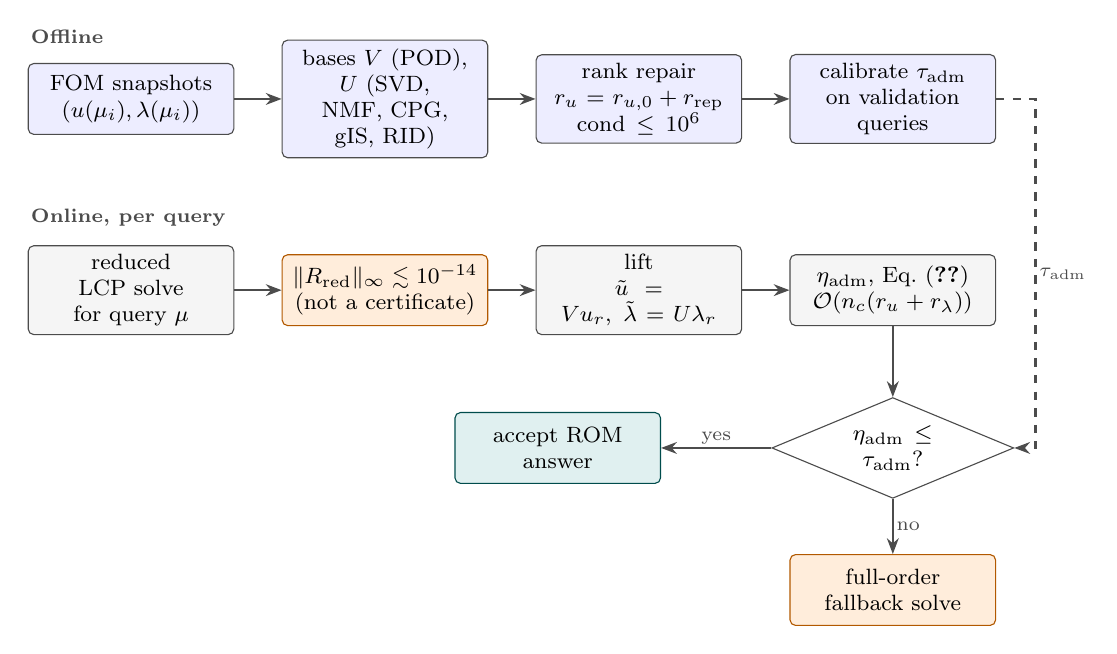
\begin{tikzpicture}[
    font=\footnotesize,
    node distance=5mm and 6mm,
    box/.style={draw=black!70, rounded corners=2pt, align=center, minimum height=9mm, text width=24mm, inner sep=3pt, fill=white},
    off/.style={box, fill=blue!7},
    on/.style={box, fill=black!4},
    bad/.style={box, fill=orange!14, draw=orange!70!black},
    good/.style={box, fill=teal!12, draw=teal!60!black},
    dec/.style={draw=black!70, diamond, aspect=2.4, align=center, inner sep=0pt, text width=17mm, fill=white},
    arr/.style={-{Stealth[length=2mm]}, thick, black!70},
    lab/.style={font=\scriptsize, black!70, inner sep=1pt}
]
% ---------- offline row ----------
\node[off] (snap) {FOM snapshots\\$(u(\mu_i),\lambda(\mu_i))$};
\node[off, right=of snap] (basis) {bases $V$ (POD),\\$U$ (SVD, NMF, CPG,\\gIS, RID)};
\node[off, right=of basis] (repair) {rank repair\\$r_u=r_{u,0}+r_{\mathrm{rep}}$\\$\mathrm{cond}\le 10^{6}$};
\node[off, right=of repair] (calib) {calibrate $\tau_{\mathrm{adm}}$\\on validation\\queries};
\draw[arr] (snap) -- (basis);
\draw[arr] (basis) -- (repair);
\draw[arr] (repair) -- (calib);
% ---------- online row ----------
\node[on, below=14mm of snap] (solve) {reduced LCP solve\\for query $\mu$};
\node[bad, right=of solve] (kkt) {$\|R_{\mathrm{red}}\|_\infty\lesssim10^{-14}$\\(not a certificate)};
\node[on, right=of kkt] (lift) {lift\\$\tilde u=Vu_r,\ \tilde\lambda=U\lambda_r$};
\node[on, right=of lift] (eta) {$\eta_{\mathrm{adm}}$, Eq.~\eqref{eq:eta-adm}\\$\mathcal{O}(n_c(r_u+r_\lambda))$};
\draw[arr] (solve) -- (kkt);
\draw[arr] (kkt) -- (lift);
\draw[arr] (lift) -- (eta);
% ---------- decision ----------
\node[dec, below=9mm of eta] (decide) {$\eta_{\mathrm{adm}}\le\tau_{\mathrm{adm}}$?};
\node[good, left=14mm of decide] (accept) {accept ROM answer};
\node[box, below=7mm of decide, fill=orange!14, draw=orange!70!black] (fallback) {full-order\\fallback solve};
\draw[arr] (eta) -- (decide);
\draw[arr] (decide) -- node[lab, above] {yes} (accept);
\draw[arr] (decide) -- node[lab, right] {no} (fallback);
% the calibrated threshold (offline) feeds the decision
\draw[arr, dashed] (calib.east) -- ++(5mm,0) |- node[lab, pos=0.25, right] {$\tau_{\mathrm{adm}}$} (decide.east);
% group labels
\node[lab, anchor=south west] at ([yshift=2mm]snap.north west) {\textbf{Offline}};
\node[lab, anchor=south west] at ([yshift=2mm]solve.north west) {\textbf{Online, per query}};
\end{tikzpicture}

\caption{Overview of the proposed framework. Offline, snapshots yield the primal basis $V$ and a dual basis $U$, the primal space is enriched until the reduced Schur complement is well conditioned, and the threshold $\tau_{\mathrm{adm}}$ is calibrated on validation queries. Online, a reduced LCP solve is followed by lifting and by the interface-only indicator $\eta_{\mathrm{adm}}$; a query is accepted only if the indicator stays below the threshold, otherwise it falls back to the full-order solver. A small reduced KKT residual alone is not a certificate of admissibility of the lifted pair.}
\label{fig:workflow}
\end{figure}

The remainder of the paper is organized as follows. Section~\ref{sec:formulation} states the full-order and reduced mixed contact formulations and illustrates silent failure. Section~\ref{sec:estimator} derives the four-component \emph{a posteriori} error bound and its online admissibility indicator. Section~\ref{sec:basis_cost} reviews the five dual-basis constructions, formulates the break-even cost model and states the offline and online procedure. Section~\ref{sec:experiments} presents numerical experiments across 1D chain, 2D obstacle membrane, and 3D two-body contact benchmarks, and Section~\ref{sec:conclusion} summarizes practical guidelines for selecting and assessing contact ROMs.

% ======================================================================
\section{Problem Formulation and Silent Failure}
\label{sec:formulation}

In a frictionless unilateral contact problem, a deformable body interacts with a rigid obstacle under an applied load. The interaction is compressive: the normal contact pressure is non-negative, interpenetration is prohibited, and the pressure vanishes wherever a positive gap exists (complementarity). After discretization, the unknowns are the nodal displacements and the contact pressures, which are represented as Lagrange multipliers attached to candidate contact points; this gives the mixed problem below. A reduced model that approximates both fields may violate one or more of these conditions after reconstruction in the full-order space, and this section describes how.

\hypertarget{full-order-discrete-unilateral-contact-problem}{%
\subsection{Full-Order Discrete Unilateral Contact Problem}\label{full-order-discrete-unilateral-contact-problem}}

Consider a parametrized linear-elastic or quasi-static discrete mechanical system with \(N\) displacement degrees of freedom and \(n_c\) unilateral contact constraints (\(n_c \le N\)) \cite{kikuchi1988contact, coorevits2000posteriori, hild2007residual}. For a parameter vector \(\mu \in \mathcal{P} \subset \mathbb{R}^{n_p}\), the full-order equilibrium and non-penetration conditions are governed by the constrained quadratic minimization problem \cite{balajewicz2016projection, benaceur2020reduced}:
\begin{equation}\label{eq:primal}\min_{u \in \mathcal{K}(\mu)} \frac{1}{2} u^T K(\mu) u - f(\mu)^T u, \qquad \mathcal{K}(\mu) := \left\{ v \in \mathbb{R}^N : B(\mu) v - c(\mu) \le 0 \right\},\end{equation}
where \(K(\mu) \in \mathbb{R}^{N \times N}\) is the symmetric positive definite (SPD) stiffness matrix, \(f(\mu) \in \mathbb{R}^N\) is the external load vector, \(B(\mu) \in \mathbb{R}^{n_c \times N}\) is a rectangular constraint Jacobian mapping nodal displacements to normal contact gaps (arising from node-to-segment or mortar contact discretizations \cite{coorevits2000posteriori, wohlmuth2000mortar, wohlmuth2011variationally, hild2010stabilized, franceschini2022block}), and \(c(\mu) \in \mathbb{R}^{n_c}\) is the initial gap vector. Throughout this work, inequalities on vectors are understood componentwise.

Let \(\lambda \in \mathbb{R}^{n_c}\) denote the contact Lagrange multipliers, which represent normal contact tractions. The first-order optimality conditions then take the mixed Karush--Kuhn--Tucker (KKT) saddle-point form \cite{hild2007residual, banz2024generic}: find \((u(\mu), \lambda(\mu)) \in \mathbb{R}^N \times \mathbb{R}^{n_c}\) such that
\begin{equation}\label{eq:kkt}\begin{aligned}
K(\mu) u(\mu) + B(\mu)^T \lambda(\mu) &= f(\mu), \\
\lambda(\mu) &\ge 0, \\
B(\mu) u(\mu) - c(\mu) &\le 0, \\
\lambda(\mu)^T \bigl(B(\mu) u(\mu) - c(\mu)\bigr) &= 0.
\end{aligned}\end{equation}
Eliminating the displacement, \(u(\mu) = K(\mu)^{-1}(f(\mu) - B(\mu)^T \lambda(\mu))\), from the equilibrium equation and substituting it into the contact conditions gives the following condensed (Schur-complement) linear complementarity problem (LCP) for the multiplier vector \cite{balajewicz2016projection, leberre2022condition}:
\begin{equation}\label{eq:lcp}\begin{aligned}
w(\mu) &:= B(\mu) K(\mu)^{-1} B(\mu)^T \lambda(\mu) + \bigl(c(\mu) - B(\mu) K(\mu)^{-1} f(\mu)\bigr) \ge 0, \\
\lambda(\mu) &\ge 0, \qquad \lambda(\mu)^T w(\mu) = 0.
\end{aligned}\end{equation}
We assume that the admissible set is non-empty for every \(\mu \in \mathcal{P}\), that is, \(\{v : B(\mu) v \le c(\mu)\} \neq \emptyset\); this holds, for example, whenever \(c(\mu) \ge 0\), since then \(v = 0\) is admissible, which is the case in all our benchmarks. The set \(\mathcal{K}(\mu)\) is then a non-empty closed convex polyhedron. Because the constraints are linear, a KKT multiplier \(\lambda(\mu)\) exists without further constraint qualifications. Because \(K(\mu)\) is SPD, a unique primal solution \(u(\mu)\) exists for every \(\mu \in \mathcal{P}\). Uniqueness of \(\lambda(\mu)\) holds whenever the active rows of \(B(\mu)\) have full row rank, which is satisfied on standard non-redundant contact interfaces \cite{wohlmuth2011variationally, franceschini2022block}.

\hypertarget{galerkinpetrov-mixed-reduced-order-model}{%
\subsection{Galerkin--Petrov Mixed Reduced-Order Model}\label{galerkinpetrov-mixed-reduced-order-model}}

To construct a projection-based reduced-order model, we collect \(n_s\) full-order snapshot pairs \(\{(u(\mu_i), \lambda(\mu_i))\}_{i=1}^{n_s}\) over a training set \(\mathcal{P}_{\text{train}} \subset \mathcal{P}\) \cite{balajewicz2016projection, benaceur2020reduced}. From these snapshots, we build a primal displacement basis \(V \in \mathbb{R}^{N \times r_u}\) with orthonormal columns (\(V^T V = I_{r_u}\), \(r_u \ll N\)) and a dual multiplier basis \(U \in \mathbb{R}^{n_c \times r_\lambda}\) (\(r_\lambda \le n_c\)) \cite{balajewicz2016projection, benaceur2020reduced, fauque2018hybrid, sambataro2026model}.

Approximating the primal and dual variables in the reduced subspaces via
\begin{equation}\label{eq:lift}u(\mu) \approx \tilde{u}(\mu) := V u_r(\mu), \qquad \lambda(\mu) \approx \tilde{\lambda}(\mu) := U \lambda_r(\mu),\end{equation}
and testing the equilibrium and gap equations with \(V^T\) and \(U^T\), respectively, yields the reduced mixed KKT system \cite{balajewicz2016projection, leberre2022condition}: find \((u_r(\mu), \lambda_r(\mu)) \in \mathbb{R}^{r_u} \times \mathbb{R}^{r_\lambda}\) such that
\begin{equation}\label{eq:red-kkt}\begin{aligned}
K_r(\mu) u_r(\mu) + B_r(\mu)^T \lambda_r(\mu) &= f_r(\mu), \\
\lambda_r(\mu) &\ge 0, \\
B_r(\mu) u_r(\mu) - c_r(\mu) &\le 0, \\
\lambda_r(\mu)^T \bigl(B_r(\mu) u_r(\mu) - c_r(\mu)\bigr) &= 0,
\end{aligned}\end{equation}
where the reduced operators are defined by
\begin{equation}\label{eq:red-ops}\begin{aligned}
K_r(\mu) &:= V^T K(\mu) V \in \mathbb{R}^{r_u \times r_u}, & B_r(\mu) &:= U^T B(\mu) V \in \mathbb{R}^{r_\lambda \times r_u}, \\
f_r(\mu) &:= V^T f(\mu) \in \mathbb{R}^{r_u}, & c_r(\mu) &:= U^T c(\mu) \in \mathbb{R}^{r_\lambda}.
\end{aligned}\end{equation}
Because \(V\) has full column rank and \(K(\mu)\) is SPD, \(K_r(\mu)\) is SPD, and the reduced system admits the Schur-complement LCP formulation \cite{balajewicz2016projection, leberre2022condition}:
\begin{equation}\label{eq:red-lcp}\begin{aligned}
w_r(\mu) &:= B_r(\mu) K_r(\mu)^{-1} B_r(\mu)^T \lambda_r(\mu) + \bigl(c_r(\mu) - B_r(\mu) K_r(\mu)^{-1} f_r(\mu)\bigr) \ge 0, \\
\lambda_r(\mu) &\ge 0, \qquad \lambda_r(\mu)^T w_r(\mu) = 0.
\end{aligned}\end{equation}

\hypertarget{mechanisms-of-silent-reduced-kkt-failure}{%
\subsection{Mechanisms of Silent Failure}\label{mechanisms-of-silent-reduced-kkt-failure}}

Enforcing the projected KKT conditions to machine precision does \textbf{not} imply physical admissibility of the lifted pair \((\tilde{u}(\mu), \tilde{\lambda}(\mu))\). Specifically, define the reduced KKT residual vector:
\begin{equation}\label{eq:resid}R_{\text{red}}(u_r, \lambda_r) := \begin{bmatrix}
\Vert K_r u_r + B_r^T \lambda_r - f_r \Vert_2 \\
\Vert \min(\lambda_r, 0) \Vert_2 \\
\Vert \max(B_r u_r - c_r, 0) \Vert_2 \\
\vert \lambda_r^T (B_r u_r - c_r) \vert
\end{bmatrix}.\end{equation}
Even when \(\Vert R_{\text{red}}(u_r, \lambda_r) \Vert_\infty \le 10^{-12}\), the lifted solution can exhibit large errors through three coupled algebraic mechanisms:

\begin{enumerate}
\def\labelenumi{\arabic{enumi}.}
\tightlist
\item
  \textbf{Loss of Dual Cone Preservation (Signed Dual Bases):}
  When \(U\) is obtained via standard truncated SVD or POD of multiplier snapshots, its columns contain mixed positive and negative entries \cite{balajewicz2016projection, benaceur2020reduced}. Consequently, \(\lambda_r \ge 0\) does not guarantee \(\tilde{\lambda} = U \lambda_r \ge 0\). Negative components in \(\tilde{\lambda}\) correspond to non-physical tensile tractions that pull the body across the contact boundary and can balance the projected equilibrium equation \(V^T(K \tilde{u} + B^T \tilde{\lambda} - f) = 0\).
\item
  \textbf{Projected Penetration Masking:}
  The reduced non-penetration condition \(U^T (B \tilde{u} - c) \le 0\) constrains only \(r_\lambda\) weighted averages of the \(n_c\) physical gaps \cite{fauque2018hybrid, sambataro2026model}. When \(r_\lambda < n_c\), positive penetrations \((B \tilde{u} - c)_i > 0\) at active contact nodes can cancel against large negative gaps \((B \tilde{u} - c)_j < 0\) at inactive nodes in the inner product \(U^T(B\tilde{u} - c)\).
\item
  \textbf{Reduced Inf-Sup Rank Deficiency:}
  Even when \(B(\mu)\) has full row rank on the active contact set, the projected matrix \(B_r(\mu) = U^T B(\mu) V\) can become rank-deficient or severely ill-conditioned if \(V\) lacks sufficient normal-displacement resolution on the contact interface \cite{benaceur2020reduced, leberre2022condition}. In that case, \(B_r K_r^{-1} B_r^T\) is singular or nearly singular, allowing large spurious vectors in \(\ker(B_r^T)\) to enter \(\lambda_r\) with negligible change to the reduced residual \cite{leberre2022condition}.
\end{enumerate}

\hypertarget{illustrative-benchmark-evidence}{%
\subsubsection{Illustrative Benchmark Evidence}\label{illustrative-benchmark-evidence}}

To make this failure concrete, consider the parametrized 2D obstacle membrane (\(N = 324\)) \cite{benaceur2020reduced} and 1D discrete spring-chain contact (\(N = 60\)) \cite{pawar2025efficient} benchmarks used in the experiments of Section~\ref{sec:experiments}. When reduced with identical primal and dual dimensions \((r_u, r_\lambda)\) using a standard signed SVD dual basis, the active-set LCP solver converges to reduced KKT residuals below \(10^{-14}\) on every test query. Upon lifting, however, the signed SVD model exhibits lifted multipliers as negative as \(\min_i \tilde{\lambda}_i = -1.6\) (B1) and \(-0.83\) (B2) and relative energy-norm errors of order one (median \(0.96\) and \(1.05\), maximum \(1.9\) and \(1.8\)), whereas a non-negative matrix factorization (NMF) dual basis \cite{balajewicz2016projection} of identical rank gives median errors of \(0.4\%\) (B1) and \(4\%\) (B2) (Figure~\ref{fig:silent}). The reduced solver itself gives no indication of this failure, which motivates the lifted error bound and admissibility indicators derived in Section~\ref{sec:estimator}. Figure~\ref{fig:silent} shows the effect on the test queries of the two benchmarks. Figure~\ref{fig:multiplier} shows the corresponding multipliers, and Figure~\ref{fig:b3rom} shows the same failure in three dimensions.

\begin{figure}[htbp]
\centering
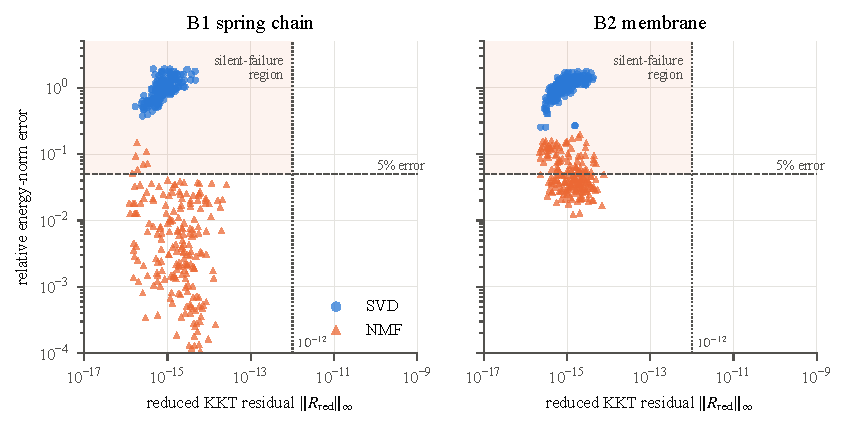
\includegraphics[width=\textwidth]{fig_silent_failure.pdf}
\caption{Silent reduced-KKT failure on B1 and B2 (200 test queries per basis: five dual dimensions $\times$ 40 parameters; the dual dimensions are pooled). Every query has a reduced KKT residual below $10^{-12}$ (residuals of exactly zero are drawn at $10^{-17}$ with a small horizontal jitter). All 200 signed-SVD queries lie in the shaded silent-failure region on both benchmarks, with a median relative energy error of about $1$. NMF errors exceed $5\%$ on $3.5\%$ of the B1 queries and on $40\%$ of the B2 queries, so non-negativity of the dual basis reduces but does not remove the hazard.}
\label{fig:silent}
\end{figure}

\begin{figure}[htbp]
\centering
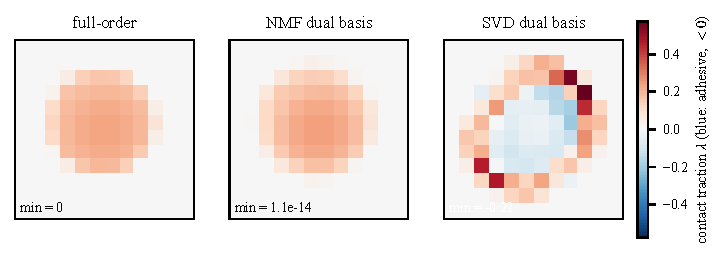
\includegraphics[width=\textwidth]{fig_multiplier.pdf}
\caption{Contact tractions on the central $12\times12$ patch of B2 for one test query, $r_\lambda=8$ with rank repair. The full-order traction (left) is non-negative, and the NMF-lifted multiplier reproduces it. The SVD-lifted multiplier is negative (tensile) inside the patch and has positive spikes at its edge; its minimum is $-0.22$ and its maximum $0.57$, against a full-order maximum of $0.23$. The color scale is symmetric about zero and shared by all panels.}
\label{fig:multiplier}
\end{figure}

% ======================================================================
\section{\emph{A Posteriori} Error Bound and Online Admissibility Indicators for Lifted Solutions}
\label{sec:estimator}

\emph{Roadmap.} Section~\ref{norms-multiplier-splitting-and-estimator-components} defines four residual indicators of a lifted pair. Section~\ref{certified-energy-norm-upper-bound} derives a rigorous energy-norm bound from them; it needs the multiplier norm and an equilibrium residual that is a full-order quantity in general, so it is a validation tool. Section~\ref{computational-complexity-and-online-admissibility-indicator} then builds the inexpensive interface-only indicators from the three terms that do not touch the bulk; these form an empirical screening indicator and carry no error guarantee. The two parts are kept apart on purpose. Terminology is used as follows. The \emph{error bound} is the mathematically derived upper bound of Section~\ref{certified-energy-norm-upper-bound}. The \emph{admissibility indicators} are the individual sign, gap and complementarity measures, and the \emph{online admissibility indicator} is their combination in Section~\ref{computational-complexity-and-online-admissibility-indicator}. The \emph{screening threshold} is the calibrated value against which the online indicator is compared, and a \emph{fallback solve} is the full-order solve performed for a rejected prediction. The terms estimator and certificate are not used for the online indicator.

To detect silent failures without solving the full-order contact problem, we derive a residual-based \emph{a posteriori} error bound for arbitrary lifted primal--dual pairs \((\tilde{u}, \tilde{\lambda}) = (V u_r, U \lambda_r)\). Existing reduced-basis error estimates for variational inequalities require a bijective constraint operator and strictly feasible dual spaces \cite{zhang2014duality}. The present analysis applies to general rectangular constraint matrices \(B(\mu) \in \mathbb{R}^{n_c \times N}\) and makes no assumption on how \((u_r, \lambda_r)\) is computed or on whether \(U\) preserves non-negativity \cite{banz2024generic, banz2026posteriori}.

\hypertarget{norms-multiplier-splitting-and-estimator-components}{%
\subsection{Norms, Multiplier Splitting, and Estimator Components}\label{norms-multiplier-splitting-and-estimator-components}}

For a fixed parameter \(\mu \in \mathcal{P}\), suppress the explicit \(\mu\)-dependence for brevity and write \(K = K(\mu)\), \(B = B(\mu)\), \(c = c(\mu)\), and \(f = f(\mu)\). Since \(K \in \mathbb{R}^{N \times N}\) is SPD, it induces the standard energy norm and dual energy norm \cite{hild2007residual, zhang2014duality}
\begin{equation}\label{eq:norms}
\|v\|_K := \left( v^T K v \right)^{1/2}, \qquad \|r\|_{K^{-1}} := \left( r^T K^{-1} r \right)^{1/2} = \sup_{v \in \mathbb{R}^N \setminus \{0\}} \frac{r^T v}{\|v\|_K}.
\end{equation}
Similarly, define the discrete trace operator norm of \(B\) with respect to the energy norm \cite{coorevits2000posteriori, hild2007residual}:
\begin{equation}\label{eq:tracenorm}
\|B\|_{K \to 2} := \sup_{v \in \mathbb{R}^N \setminus \{0\}} \frac{\|B v\|_2}{\|v\|_K} = \left\| B K^{-1} B^T \right\|_2^{1/2}.
\end{equation}
For any vector \(z \in \mathbb{R}^{n_c}\), denote its componentwise positive and negative parts by \(z_+ := \max(z, 0) \ge 0\) and \(z_- := \min(z, 0) \le 0\), so that \(z = z_+ + z_-\) and \(z_+^T z_- = 0\).

We split the lifted Lagrange multiplier \(\tilde{\lambda} = U \lambda_r\) into its physically admissible (compressive) part and its non-physical (negative, tensile) part. The splitting follows the constant-sign multiplier decomposition and the non-Galerkin residual splitting introduced for full-order mixed contact and variational inequalities \cite{hild2007residual, dabaghi2020posteriori, banz2024generic, banz2026posteriori}; see also \cite{haasdonk2012reduced} for reduced-basis variational inequalities with a posteriori bounds:
\begin{equation}\label{eq:split}
\tilde{\lambda} = \lambda_+ + \lambda_-, \qquad \lambda_+ := \max(\tilde{\lambda}, 0), \qquad \lambda_- := \min(\tilde{\lambda}, 0).
\end{equation}
Sign convention: the constraint is \(B u - c \le 0\) and \(\lambda \ge 0\), so a positive multiplier component is a compressive contact traction and \(\lambda_+\) is its admissible part, while \(\lambda_- \le 0\) collects the non-physical negative (tensile) components (the reduction packages used in our code use the opposite sign for both \(B\) and \(\lambda\); we convert before evaluating any indicator). Accordingly \(\eta_{\mathrm{sign}} = \|\lambda_-\|_2\) is the norm of the negative multiplier component, \((B\tilde{u} - c)_+\) collects penetrations, and \(\lambda_+\), \(\lambda_-\) have disjoint supports. Using \(\lambda_+\) as a feasible dual proxy \cite{hild2007residual, fontana2024guaranteed}, we define four computable residual indicators for the lifted pair \((\tilde{u}, \tilde{\lambda})\):
\begin{equation}\label{eq:indicators}
\begin{aligned}
\eta_{\mathrm{eq}} &:= \left\| K \tilde{u} + B^T \lambda_+ - f \right\|_{K^{-1}}, & \eta_{\mathrm{sign}} &:= \left\| \lambda_- \right\|_2, \\
\eta_{\mathrm{gap}} &:= \left\| (B \tilde{u} - c)_+ \right\|_2, & \eta_{\mathrm{comp}} &:= \left| \lambda_+^T (B \tilde{u} - c) \right|.
\end{aligned}
\end{equation}
Each component isolates a distinct physical or algebraic defect of the lifted solution \cite{dabaghi2020posteriori, banz2024generic, fontana2024guaranteed}:
\begin{itemize}
\tightlist
\item \(\eta_{\mathrm{eq}}\) measures the bulk force-balance residual when only the non-negative part \(\lambda_+\) of the lifted traction is applied \cite{hild2007residual};
\item \(\eta_{\mathrm{sign}}\) quantifies the violation of multiplier non-negativity as the Euclidean norm of the negative component (\(\tilde{\lambda}_i < 0\)) \cite{balajewicz2016projection, banz2026posteriori};
\item \(\eta_{\mathrm{gap}}\) measures the Euclidean norm of positive interpenetration across all \(n_c\) candidate contact constraints \cite{coorevits2000posteriori, hild2007residual};
\item \(\eta_{\mathrm{comp}}\) measures the violation of complementarity slackness between the compressive tractions \(\lambda_+\) and the physical gap vector \(B \tilde{u} - c\) \cite{dabaghi2020posteriori, banz2024generic}.
\end{itemize}

\hypertarget{certified-energy-norm-upper-bound}{%
\subsection{Energy-Norm Upper Bound}\label{certified-energy-norm-upper-bound}}

Adapting the primal--dual contact error decomposition of Hild and Nicaise \cite{hild2007residual} and Banz et al.~\cite{banz2024generic, banz2026posteriori} to lifted reduced-order pairs without Galerkin orthogonality, the following theorem establishes that the energy-norm displacement error \(\|u - \tilde{u}\|_K\) is bounded from above by these four quantities and the multiplier norm \(\|\lambda\|_2\).

\begin{theorem}[Residual-Based \emph{A Posteriori} Error Bound for Lifted Contact Pairs]\label{thm:bound}

Let \(K\) be symmetric positive definite, let the admissible set \(\{v : B v \le c\}\) be non-empty, let \((u, \lambda) \in \mathbb{R}^N \times \mathbb{R}^{n_c}\) be a KKT solution of the discrete contact problem~\eqref{eq:kkt}, and let \((\tilde{u}, \tilde{\lambda}) = (V u_r, U \lambda_r)\) be any lifted reduced-order approximation. Then the energy-norm displacement error satisfies
\begin{equation}\label{eq:bound1}
\|u - \tilde{u}\|_K^2 \le \eta_{\mathrm{eq}}^2 + 2\,\eta_{\mathrm{comp}} + 2\,\|\lambda\|_2\,\eta_{\mathrm{gap}}.
\end{equation}
Furthermore, letting \(\tilde{r}_{\mathrm{eq}} := \|K \tilde{u} + B^T \tilde{\lambda} - f\|_{K^{-1}}\) denote the equilibrium residual evaluated with the unprojected lifted multiplier \(\tilde{\lambda}\), the error bound decomposes explicitly into all four indicators:
\begin{equation}\label{eq:bound2}
\|u - \tilde{u}\|_K^2 \le 2\,\tilde{r}_{\mathrm{eq}}^2 + 2\,\|B\|_{K \to 2}^2\,\eta_{\mathrm{sign}}^2 + 2\,\eta_{\mathrm{comp}} + 2\,\|\lambda\|_2\,\eta_{\mathrm{gap}}.
\end{equation}

\end{theorem}

\begin{proof}

Let \(e := u - \tilde{u} \in \mathbb{R}^N\). Using the exact equilibrium relation \(K u = f - B^T \lambda\) and adding and subtracting \(B^T \lambda_+\), we expand the squared energy-norm error as \cite{hild2007residual, banz2024generic}

\[
\begin{aligned}
\|e\|_K^2 &= e^T K (u - \tilde{u}) \\
&= e^T \left( f - B^T \lambda - K \tilde{u} \right) \\
&= e^T \left( f - K \tilde{u} - B^T \lambda_+ \right) + (B e)^T (\lambda_+ - \lambda).
\end{aligned}
\]
For the first term, applying the Cauchy--Schwarz inequality in the \(K\)-inner product followed by Young's inequality (\(a b \le \frac{1}{2} a^2 + \frac{1}{2} b^2\)) yields
\[
e^T \left( f - K \tilde{u} - B^T \lambda_+ \right) \le \|e\|_K \, \left\| K \tilde{u} + B^T \lambda_+ - f \right\|_{K^{-1}} = \|e\|_K \, \eta_{\mathrm{eq}} \le \frac{1}{2} \|e\|_K^2 + \frac{1}{2} \eta_{\mathrm{eq}}^2.
\]
For the second term, rewrite \(B e = (B u - c) - (B \tilde{u} - c)\) and expand the inner product into four contributions \cite{hild2007residual, banz2026posteriori}:
\[
(B e)^T (\lambda_+ - \lambda) = (B u - c)^T \lambda_+ - (B u - c)^T \lambda - (B \tilde{u} - c)^T \lambda_+ + (B \tilde{u} - c)^T \lambda.
\]
By full-order primal feasibility (\(B u - c \le 0\)) and non-negativity of \(\lambda_+\) (\(\lambda_+ \ge 0\)), the first inner product is non-positive: \((B u - c)^T \lambda_+ \le 0\). By exact full-order complementarity, the second inner product vanishes identically: \((B u - c)^T \lambda = 0\). Dropping these two non-positive terms gives
\[
(B e)^T (\lambda_+ - \lambda) \le -(B \tilde{u} - c)^T \lambda_+ + (B \tilde{u} - c)^T \lambda.
\]
The third term is bounded by \(\left| \lambda_+^T (B \tilde{u} - c) \right| = \eta_{\mathrm{comp}}\). This step uses \(-x \le |x|\) and is therefore valid whichever sign the inner product \(\lambda_+^T (B \tilde{u} - c)\) has. The absolute value in the definition of \(\eta_{\mathrm{comp}}\) is essential: it makes the indicator non-negative, so that \(\sqrt{\eta_{\mathrm{comp}}}\) is real, and it covers the case in which \(\lambda_+\) is not complementary to the gap of a lifted displacement. That case does occur: on the audited queries the inner product was negative for 90 of 200 queries on B1 and for 74 of 200 on B2 (five dual bases, two dual dimensions, 20 queries each), and \eqref{eq:bound1} held on all of them. For the fourth term, decompose \(B \tilde{u} - c = (B \tilde{u} - c)_+ + (B \tilde{u} - c)_-\). Since \(\lambda \ge 0\) and \((B \tilde{u} - c)_- \le 0\), we have \((B \tilde{u} - c)_-^T \lambda \le 0\), and hence by the Euclidean Cauchy--Schwarz inequality,
\[
(B \tilde{u} - c)^T \lambda \le (B \tilde{u} - c)_+^T \lambda \le \|\lambda\|_2 \, \left\| (B \tilde{u} - c)_+ \right\|_2 = \|\lambda\|_2 \, \eta_{\mathrm{gap}}.
\]
Combining these bounds into the expansion of \(\|e\|_K^2\) gives
\[
\|e\|_K^2 \le \frac{1}{2} \|e\|_K^2 + \frac{1}{2} \eta_{\mathrm{eq}}^2 + \eta_{\mathrm{comp}} + \|\lambda\|_2 \, \eta_{\mathrm{gap}}.
\]
Subtracting \(\frac{1}{2} \|e\|_K^2\) from both sides and multiplying by \(2\) establishes \eqref{eq:bound1}.

To obtain \eqref{eq:bound2}, substitute \(\lambda_+ = \tilde{\lambda} - \lambda_-\) into \(\eta_{\mathrm{eq}}\) and apply the triangle inequality together with \((a + b)^2 \le 2 a^2 + 2 b^2\):
\[
\eta_{\mathrm{eq}}^2 = \left\| \left( K \tilde{u} + B^T \tilde{\lambda} - f \right) - B^T \lambda_- \right\|_{K^{-1}}^2 \le 2\,\tilde{r}_{\mathrm{eq}}^2 + 2\,\left\| B^T \lambda_- \right\|_{K^{-1}}^2.
\]
By definition of the dual energy norm and the trace norm \(\|B\|_{K \to 2}\) \cite{coorevits2000posteriori, franceschini2022block},
\[
\left\| B^T \lambda_- \right\|_{K^{-1}} = \sup_{v \in \mathbb{R}^N \setminus \{0\}} \frac{\lambda_-^T B v}{\|v\|_K} \le \sup_{v \in \mathbb{R}^N \setminus \{0\}} \frac{\|\lambda_-\|_2 \, \|B v\|_2}{\|v\|_K} = \|B\|_{K \to 2} \, \eta_{\mathrm{sign}}.
\]
Inserting this estimate into \eqref{eq:bound1} yields \eqref{eq:bound2}. \(\blacksquare\)

\end{proof}

\begin{remark}[Practical Evaluation of Constants and $\|\lambda\|_2$]

In \eqref{eq:bound1}--\eqref{eq:bound2}, the exact multiplier norm \(\|\lambda\|_2\) is unknown online. When \(B\) has full row rank with full-order discrete inf-sup constant \(\beta > 0\) (i.e., \(\inf_{\mu_c \neq 0} \sup_{v \neq 0} \mu_c^T B v / (\|\mu_c\|_2 \|v\|_K) \ge \beta\)), standard saddle-point stability \cite{brezzi1991mixed, hild2007residual, franceschini2022block} bounds \(\|\lambda\|_2 \le \beta^{-1} (\|f\|_{K^{-1}} + \|K u\|_{K^{-1}}) \le 2 \beta^{-1} \|f\|_{K^{-1}}\) (the last step uses \(c \ge 0\), a non-negative initial gap, which holds in all our benchmarks). Three evaluations of \(\|\lambda\|_2\) are possible in practice. (i) The exact norm from a full-order solve is available only for validation; it is what the effectivity and correlation results of Section~\ref{sec:experiments} use (the ``exact-norm'' bound). (ii) The offline constant \(C_\lambda = \max_{\mu \in \mathcal{P}_{\mathrm{train}}} \|\lambda(\mu)\|_2\) gives a bound usable online that is rigorous whenever \(\|\lambda(\mu)\|_2 \le C_\lambda\), that is, in the interpolation regime, and can fail outside it. (iii) The computable proxy \(\|\tilde{\lambda}_+\|_2\) carries no guarantee, because it need not bound the exact multiplier norm; we do not use it. The stability bound of the previous paragraph is rigorous but conservative. On 20 test queries per benchmark, \(\beta^{-1}(\|f\|_{K^{-1}} + \|u\|_K)\) reached 20.1 (B1) and 26.2 (B2), with \(\beta_{\min} = 0.70\) and \(0.36\), against largest true multiplier norms of 2.09 and 1.63 and offline constants \(C_\lambda\) of 2.37 and 1.64. It is thus a defensible but roughly tenfold looser alternative to \(C_\lambda\), and it would inflate the gap term of the bound by the same factor. \(C_\lambda\) is the sharper choice inside the training range; the inf-sup bound is the one to use when a guarantee outside the range is required and \(\beta\) can be computed offline.
\end{remark}

\begin{remark}[Why Signed SVD Fails Silently]

Bound \eqref{eq:bound2} directly explains the empirical breakdown documented in Section~\ref{mechanisms-of-silent-reduced-kkt-failure}. Even if a reduced solver drives the projected residual \(\tilde{r}_{\mathrm{eq}}\) to a small value, a signed SVD dual basis permits large negative lifted multipliers \(\lambda_- \neq 0\). The resulting sign violation \(\eta_{\mathrm{sign}} = \|\lambda_-\|_2\) enters the upper bound multiplied by \(2 \|B\|_{K \to 2}^2\), simultaneously inducing positive penetration \(\eta_{\mathrm{gap}}\) and complementarity error \(\eta_{\mathrm{comp}}\). Conversely, when a strictly non-negative dual basis is used (such as NMF \cite{balajewicz2016projection}, cone-projected greedy \cite{benaceur2020reduced}, or greedy index selection \cite{sambataro2026model}), \(\eta_{\mathrm{sign}} = 0\) identically, so that \eqref{eq:bound1} applies as stated and \eqref{eq:bound2} reduces to \(\|u - \tilde{u}\|_K^2 \le 2\,\eta_{\mathrm{eq}}^2 + 2\,\eta_{\mathrm{comp}} + 2\,\|\lambda\|_2\,\eta_{\mathrm{gap}}\), which is weaker than \eqref{eq:bound1} by a factor two in the equilibrium term.
\end{remark}

\begin{remark}[What is certified and what is empirical]

Three statements are made in this paper, and they carry different guarantees. (a) \emph{Rigorous bound.} Theorem~\ref{thm:bound}, with the exact multiplier norm \(\|\lambda\|_2\) or with any valid upper bound on it (for example the inf-sup bound of Remark~1), is a mathematical upper bound on the energy-norm error. It contains the equilibrium residual \(\eta_{\mathrm{eq}}\), which needs a solve with \(K\) unless the problem is affine, so it is a validation quantity. (b) \emph{Online-usable bound.} Replacing \(\|\lambda\|_2\) by the offline constant \(C_\lambda\) gives a bound that is rigorous only while \(\|\lambda(\mu)\|_2 \le C_\lambda\); outside the training range it is a heuristic. (c) \emph{Interface screening indicator.} The indicators \(\eta_{\mathrm{adm}}\) and \(\eta_{\mathrm{adm,v2}}\) of Section~\ref{computational-complexity-and-online-admissibility-indicator} omit \(\eta_{\mathrm{eq}}\) and are compared with a threshold \(\tau_{\mathrm{adm}}\) calibrated on validation queries. They are not error bounds: a small value does not imply a small error, because the bulk equilibrium residual can be large, and the threshold has no guarantee outside the calibration data. An accepted prediction is therefore not certified. The reliability of an accepted prediction is therefore limited to the empirical recall reported in Section~\ref{sec:experiments}. The screening indicator is intended to trigger a fallback and does not replace the bound of item (a).
\end{remark}

\hypertarget{computational-complexity-and-online-admissibility-indicator}{%
\subsection{Computational Complexity and Online Admissibility Indicator}\label{computational-complexity-and-online-admissibility-indicator}}

Evaluating the four estimator components splits naturally into a bulk equilibrium term and three contact-interface admissibility terms:

\begin{longtable}[]{@{}
  >{\raggedright\arraybackslash}p{(\columnwidth - 6\tabcolsep) * \real{0.25}}
  >{\raggedright\arraybackslash}p{(\columnwidth - 6\tabcolsep) * \real{0.25}}
  >{\raggedright\arraybackslash}p{(\columnwidth - 6\tabcolsep) * \real{0.25}}
  >{\raggedright\arraybackslash}p{(\columnwidth - 6\tabcolsep) * \real{0.25}}@{}}
\toprule
Estimator Term & Definition & Online Operation Count & Bulk \(N\)-Dependence \\
\midrule
\endhead
\(\eta_{\mathrm{sign}}\) & \(\|\min(U \lambda_r, 0)\|_2\) & \(\mathcal{O}(n_c r_\lambda)\) & None \\
\(\eta_{\mathrm{gap}}\) & \(\|\max((B V) u_r - c, 0)\|_2\) & \(\mathcal{O}(n_c r_u)\) & None (if \(B V\) precomputed) \\
\(\eta_{\mathrm{comp}}\) & \(|\lambda_+^T ((B V) u_r - c)|\) & \(\mathcal{O}(n_c)\) & None \\
\(\eta_{\mathrm{eq}}\) & \(\|K \tilde{u} + B^T \lambda_+ - f\|_{K^{-1}}\) & \(\mathcal{O}(N^\alpha)\) (general) / \(\mathcal{O}((r_u + r_\lambda)^2)\) (affine) & Full-order solve unless affine \\
\bottomrule
\end{longtable}

When the parameter dependence of \(B(\mu)\) and \(c(\mu)\) is affine (or parameter-independent, as in fixed-interface contact with varying external loads), the matrix products \(B V \in \mathbb{R}^{n_c \times r_u}\) are precomputed once offline \cite{benaceur2020reduced, zhang2014duality}. Online evaluation of \(\eta_{\mathrm{sign}}\), \(\eta_{\mathrm{gap}}\), and \(\eta_{\mathrm{comp}}\) then requires only \(\mathcal{O}(n_c (r_u + r_\lambda))\) floating-point operations---completely independent of the bulk mesh dimension \(N\). When \(B(\mu)\) or \(c(\mu)\) is not affine, the product \(B(\mu) V\) cannot be precomputed. It is then formed per query as \(B_{:,\Gamma}(\mu) V_{\Gamma,:}\), where \(\Gamma\) is the set of degrees of freedom touched by the contact rows, at the cost \(\mathcal{O}(\mathrm{nnz}(B)\, r_u)\) instead of \(\mathcal{O}(n_c r_u)\) for the product with a precomputed \(BV\); for node-to-segment type constraints with a bounded number of degrees of freedom per row this is still of order \(n_c r_u\) and independent of \(N\), but the constant grows with the stencil. Only the rows of \(V\) on \(\Gamma\) are needed online. In our benchmarks \(B\) does not depend on \(\mu\), while \(c\) does and enters as a vector.

For \(\eta_{\mathrm{eq}}\), computing the dual norm \(\|r\|_{K^{-1}}\) in general non-affine problems requires a full-order linear solve with \(K\), making \(\eta_{\mathrm{eq}}\) an offline validation metric or greedy snapshot-selection criterion rather than an online diagnostic. In strictly affine settings, \(\eta_{\mathrm{eq}}^2\) can be evaluated online in \(\mathcal{O}((r_u + r_\lambda)^2)\) operations via standard offline--online Riesz representation of the residual components \cite{zhang2014duality, benaceur2020reduced}, though we reserve \(\eta_{\mathrm{eq}}\) for validation in our general framework.

To provide a fast online ``circuit breaker'' that operates solely on the contact interface \cite{dabaghi2020posteriori, fauque2018hybrid}, we combine the three \(\mathcal{O}(n_c (r_u + r_\lambda))\) terms into the \textbf{Online Admissibility Indicator}:
\begin{equation}\label{eq:eta-adm}
\eta_{\mathrm{adm}}(\tilde{u}, \tilde{\lambda}) := \eta_{\mathrm{sign}} + \eta_{\mathrm{gap}} + \sqrt{\eta_{\mathrm{comp}}}.
\end{equation}
Taking the square root of \(\eta_{\mathrm{comp}}\) makes the three terms scale with the first power of the error \(\mathcal{O}(\|e\|_K)\) in the sense of the order of smallness, matching the scaling of \(\|u - \tilde{u}\|_K\) in Theorem~\ref{thm:bound}. It does \emph{not} make the sum dimensionally consistent: \(\eta_{\mathrm{sign}}\) has the units of a multiplier (force or traction), \(\eta_{\mathrm{gap}}\) those of a displacement, and \(\sqrt{\eta_{\mathrm{comp}}}\) those of the square root of a force times a displacement, which is the unit of the energy norm. Under a change of the force unit by a factor \(s\) (\(K, f, \lambda\) scale by \(s\); displacements and gaps are unchanged) the three terms scale by \(s\), \(1\) and \(\sqrt{s}\), so the relative weight of the terms, and hence the meaning of one value of \(\tau_{\mathrm{adm}}\), changes with the units and with the load and stiffness scale. Equation~\eqref{eq:eta-adm} is therefore a heuristic whose threshold must be recalibrated whenever the scales change.

The dimensionally consistent alternative is the interface part of bound~\eqref{eq:bound2},
\begin{equation}\label{eq:eta-adm-v2}
\eta_{\mathrm{adm,v2}} := \Bigl(2\,\|B\|_{K \to 2}^2\,\eta_{\mathrm{sign}}^2 + 2\,\eta_{\mathrm{comp}} + 2\,C_\lambda\,\eta_{\mathrm{gap}}\Bigr)^{1/2},
\end{equation}
in which the exact multiplier norm is replaced by the offline constant \(C_\lambda\) and the trace constant \(\|B\|_{K \to 2}\) is precomputed offline (for parameter-dependent \(B\) it is recomputed or bounded offline over the parameter domain). Every term under the root has the units of force times displacement, so \(\eta_{\mathrm{adm,v2}}\) has the units of the energy norm; under a force-unit change by \(s\) it scales by \(\sqrt{s}\), exactly like \(\|u - \tilde{u}\|_K\), so a relative threshold \(\tau_{\mathrm{adm}}/\|u\|_K\) is unit-independent. Its online cost is the same \(\mathcal{O}(n_c (r_u + r_\lambda))\), and it is reported alongside Eq.~\eqref{eq:eta-adm} in Section~\ref{sec:experiments}. Neither indicator contains \(\eta_{\mathrm{eq}}\), so neither is an error bound (Remark~3). When an indicator exceeds the screening threshold \(\tau_{\mathrm{adm}}\), the reduced prediction is rejected, even if the projected KKT residual is at machine precision, and either the basis is enriched or the full-order solver is invoked as a fallback.

% ======================================================================
\section{Dual-Basis Constructions and Break-Even Cost Model}
\label{sec:basis_cost}

\emph{Why the dual basis matters for both admissibility and cost.} The dual basis $U$ decides whether the lifted multipliers can be negative (a signed basis can, a non-negative one cannot), how many contact rows the reduced model carries, and how much the primal space must be enlarged to keep the reduced Schur complement well conditioned. The first effect governs admissibility and accuracy, the other two govern the online cost through the dense reduced algebra, so the two cannot be assessed separately.

Sections 2 and 3 established that the reliability of a Lagrange-multiplier contact ROM hinges on the interplay between the dual basis \(U \in \mathbb{R}^{n_c \times r_\lambda}\), the primal enrichment required to keep \(B_r(\mu) = U^T B(\mu) V\) well-conditioned \cite{benaceur2020reduced, leberre2022condition}, and the resulting online computational cost. In this section, we first unify the five major dual-basis constructions within a common algebraic notation and then formulate an explicit FLOP- and iteration-aware break-even cost model comparing the enriched ROM against a sparse full-order contact solver \cite{franceschini2022block, pawar2025efficient}.

\hypertarget{unified-summary-of-dual-basis-constructions}{%
\subsection{Unified Summary of Dual-Basis Constructions}\label{unified-summary-of-dual-basis-constructions}}

Let \(\Lambda_{\text{snap}} = [\lambda(\mu_1), \dots, \lambda(\mu_{n_s})] \in \mathbb{R}_{\ge 0}^{n_c \times n_s}\) denote the matrix of non-negative multiplier snapshots collected over \(\mathcal{P}_{\text{train}}\), and let \(V_0 \in \mathbb{R}^{N \times r_{u,0}}\) be an initial orthonormal POD basis of the displacement snapshots \(U_{\text{snap}} = [u(\mu_1), \dots, u(\mu_{n_s})]\) \cite{balajewicz2016projection, benaceur2020reduced}. Each of the five dual-basis strategies constructs \(U \in \mathbb{R}^{n_c \times r_\lambda}\)---and, where necessary, enriches \(V_0\) to \(V \in \mathbb{R}^{N \times r_u}\)---as follows:

\begin{enumerate}
\def\labelenumi{\arabic{enumi}.}
\item
  \textbf{Signed SVD with Primal Rank Repair (SVD+Repair).}
  \emph{Construction:} \(U\) consists of the leading \(r_\lambda\) left singular vectors of \(\Lambda_{\text{snap}}\) \cite{balajewicz2016projection, leberre2022condition}.
  \emph{Property:} The columns have mixed signs, so \(\eta_{\text{sign}}\) is not controlled by construction.
  \emph{Primal repair:} \(U^T B V_0\) frequently exhibits rank deficiency or severe ill-conditioning on active contact rows. To restore full row rank of \(B_r\), \(V_0\) is enriched with \(r_{\text{rep}}\) unit vectors or supremizer modes \(\{K^{-1} B^T u_j\}_{j=1}^{r_\lambda}\) localized at poorly resolved contact degrees of freedom, which gives \(V = [V_0, V_{\text{rep}}]\) with \(r_u = r_{u,0} + r_{\text{rep}}\) \cite{benaceur2020reduced, leberre2022condition}.
  \emph{Cost:} The offline cost is the lowest of the five (a single SVD).
\item
  \textbf{Non-Negative Matrix Factorization (NMF).}
  \emph{Construction:} Following Balajewicz et al.~\cite{balajewicz2016projection}, \(\Lambda_{\text{snap}} \approx U H\) is factored offline by projected alternating least squares or multiplicative updates, with \(U \in \mathbb{R}_{\ge 0}^{n_c \times r_\lambda}\) and \(H \in \mathbb{R}_{\ge 0}^{r_\lambda \times n_s}\) \cite{lee1999learning}.
  \emph{Property:} Because every entry of \(U\) is non-negative and \(\lambda_r \ge 0\) is enforced by the reduced KKT solver, the lifted multiplier satisfies \(\tilde{\lambda} = U \lambda_r \ge 0\) identically, so \(\eta_{\text{sign}} = 0\) for all parameters.
  \emph{Primal repair:} The columns are non-orthogonal and generally less compact than SVD modes, which often requires a larger \(r_\lambda\) and primal enrichment \(r_{\text{rep}}\) to prevent locking \cite{balajewicz2016projection, leberre2022condition}.
  \emph{Cost:} The iterative factorization makes the offline cost the highest of the five in our implementation.
\item
  \textbf{Cone-Projected Greedy Basis (CPG).}
  \emph{Construction:} Following Benaceur et al.~\cite{benaceur2020reduced}, snapshots are selected iteratively from \(\Lambda_{\text{snap}}\) by maximizing the projection residual onto the positive cone \(\text{cone}(U^{(k-1)}) = \{ \sum_{j=1}^{k-1} \alpha_j u_j : \alpha_j \ge 0 \}\). At iteration \(k\), the snapshot \(\lambda(\mu^*)\) that maximizes \(\min_{\alpha \ge 0} \Vert{}\lambda(\mu) - U^{(k-1)} \alpha\Vert{}_2\) is added as a normalized column of \(U\).
  \emph{Property:} The columns are positively scaled physical snapshots, so \(\eta_{\text{sign}} = 0\) holds identically without an iterative NMF optimization.
  \emph{Primal repair:} Linear independence of the columns can degrade as \(r_\lambda\) grows \cite{benaceur2020reduced}, which can require additional primal enrichment.
  \emph{Cost:} The offline cost is moderate (a greedy non-negative least-squares search).
\item
  \textbf{Greedy Index Selection (gIS).}
  \emph{Construction:} Following Sambataro and Ehrlacher \cite{sambataro2026model} (and related sparse contact selection approaches \cite{kollepara2024sparse}), \(U = [e_{i_1}, \dots, e_{i_{r_\lambda}}] \in \{0, 1\}^{n_c \times r_\lambda}\) is a sparse selection matrix of canonical unit vectors at \(r_\lambda\) greedily selected contact indices \(\mathcal{I} = \{i_1, \dots, i_{r_\lambda}\} \subset \{1, \dots, n_c\}\).
  \emph{Property:} This choice gives \(\eta_{\text{sign}} = 0\) and exact pointwise complementarity \((B \tilde{u} - c)_{i_k} = 0\) on the selected indices, at the cost of setting \(\tilde{\lambda}_i = 0\) for all \(i \notin \mathcal{I}\) \cite{sambataro2026model}.
  \emph{Primal repair:} The selected rows may not resolve the contact interface, and six repair vectors were needed at \(r_\lambda = 16\) in our tests.
  \emph{Cost:} Dense dual projection is eliminated, so the offline and online overheads of the dual basis are low.
\item
  \textbf{Reduced Integration Domain Restriction (RID).}
  \emph{Construction:} Following Fauque et al.~\cite{fauque2018hybrid} and Le Berre et al.~\cite{leberre2022condition} (see also empirical cubature \cite{koller2021hyper, aresdeparga2023petrov}), the contact interface and the bulk integration are restricted to a reduced domain \(\Omega_{\text{RID}}\) that retains \(n_{c,\text{RID}} \le n_c\) contact rows around high-activity regions.
  \emph{Property:} Pointwise multipliers or localized positive modes enforce \(\eta_{\text{sign}} = 0\) on the retained rows \cite{fauque2018hybrid, leberre2022condition}.
  \emph{Primal repair:} The restriction is paired with localized primal interface enrichment \(V_{\text{RID}}\) (unit vectors on the nodes of \(\Omega_{\text{RID}}\)), which required up to 78 repair vectors at nominal \(r_\lambda = 16\) in our tests.
  \emph{Cost:} Efficiency depends on keeping \(n_{c,\text{RID}} \ll n_c\); the effective dual dimension generally exceeds the nominal one.
\end{enumerate}

Algorithms~\ref{alg:cpg}--\ref{alg:rid} state the CPG, gIS and RID constructions as implemented in our experiments (the RID construction uses the discrete empirical interpolation method \cite{chaturantabut2010nonlinear}) (the signed SVD takes the leading left singular vectors of \(\Lambda_{\mathrm{snap}}\), and NMF uses the factorization routine of the reduction package), and Algorithm~\ref{alg:repair} states the supremizer rank repair that gives \(r_{\mathrm{rep}}\). The gIS strategy selects contact indices according to their accumulated multiplier energy. Because the columns of \(U\) are orthonormal, each greedy choice minimizes the multiplier energy that remains neglected. The enrichment terminates when the condition-number limit \(\kappa_{\max}\) is reached, when \(r_\lambda\) vectors have been added, or when the computed supremizer already lies in the span of \(V\). In the last two cases the limit is not attained, and the algorithm returns the enriched basis together with the condition number it achieved. The implementation records this value but does not abort. In the baseline E3 audit on B1 three entries ended above \(\kappa_{\max} = 10^{6}\) (NMF with \(r_\lambda = 24\): \(4.4\times10^{7}\); CPG with \(r_\lambda = 16\): \(6.8\times10^{7}\); CPG with \(r_\lambda = 24\): infinite, a numerically singular reduced Schur complement), and none did on B2. A reduced model with an ill-conditioned or singular Schur complement can lose accuracy in the reduced LCP solve, so such entries should not be deployed as they are: either \(r_\lambda\) should be reduced, discarding the weakest dual modes, or the primal space enlarged by other means, or the query should be sent to the full-order solver. The reported accuracy of these entries is therefore that of a model that did not meet its own conditioning target.

\begin{algorithm}[H]\small
\caption{Cone-projected greedy dual basis (CPG).}\label{alg:cpg}
\begin{algorithmic}[1]
\Require snapshots $\Lambda_{\mathrm{snap}}=[\lambda_1,\dots,\lambda_{n_s}]\in\mathbb{R}^{n_c\times n_s}_{\ge 0}$, dimension $r_\lambda$
\Ensure non-negative dual basis $U\in\mathbb{R}^{n_c\times r}_{\ge 0}$ with $r\le r_\lambda$
\State $\mathcal{S}\gets\{\arg\max_s\|\lambda_s\|_2\}$
\While{$|\mathcal{S}|<\min(r_\lambda,n_s)$}
  \ForAll{$s\notin\mathcal{S}$}
    \State $\rho_s\gets\min_{\alpha\ge 0}\|\lambda_s-\Lambda_{\mathcal{S}}\,\alpha\|_2$ \Comment{non-negative least squares}
  \EndFor
  \If{$\max_s\rho_s\le 10^{-12}$} \State \textbf{break} \EndIf
  \State $\mathcal{S}\gets\mathcal{S}\cup\{\arg\max_{s\notin\mathcal{S}}\rho_s\}$ \Comment{worst-approximated snapshot}
\EndWhile
\State \Return $U\gets\Lambda_{\mathcal{S}}\,\mathrm{diag}\big(\|\lambda_s\|_2^{-1}\big)_{s\in\mathcal{S}}$ \Comment{normalized columns}
\end{algorithmic}
\end{algorithm}
\begin{algorithm}[H]\small
\caption{Greedy index selection dual basis (gIS).}\label{alg:gis}
\begin{algorithmic}[1]
\Require snapshots $\Lambda_{\mathrm{snap}}\in\mathbb{R}^{n_c\times n_s}_{\ge 0}$, dimension $r_\lambda$
\Ensure selection matrix $U=[e_{i_1},\dots,e_{i_{r_\lambda}}]\in\{0,1\}^{n_c\times r_\lambda}$
\State $E_j\gets\sum_{s=1}^{n_s}\lambda_s[j]^2$ for $j=1,\dots,n_c$ \Comment{snapshot energy of each contact row}
\State $\mathcal{I}\gets$ the $r_\lambda$ indices with the largest $E_j$, sorted increasingly
\State \Return $U\gets I_{n_c}[:,\mathcal{I}]$
\end{algorithmic}
\end{algorithm}
\begin{algorithm}[H]\small
\caption{Reduced integration domain dual basis (RID).}\label{alg:rid}
\begin{algorithmic}[1]
\Require snapshots $\Lambda_{\mathrm{snap}}$, primal POD basis $V$, constraint matrix $B$, element connectivity, dimension $r_\lambda$, number of element rings $m$
\Ensure selection matrix $U=I_{n_c}[:,\mathcal{I}]$ on the retained contact rows $\mathcal{I}$
\State $\Phi\gets$ leading $r_\lambda$ left singular vectors of $\Lambda_{\mathrm{snap}}$
\State $\mathcal{D}_u\gets\mathrm{DEIM}\big(V_{:,1:r_\lambda}\big)$ \Comment{interpolation DOFs of the primal basis}
\State $\mathcal{R}\gets\mathrm{DEIM}(\Phi)$ \Comment{interpolation rows of the multiplier modes}
\State $\mathcal{D}_\lambda\gets$ DOFs coupled to the rows $\mathcal{R}$ through $B$
\State $\mathcal{E}\gets$ elements containing a DOF of $\mathcal{D}_u\cup\mathcal{D}_\lambda$, grown by $m$ rings of neighbouring elements
\State $\mathcal{I}\gets$ contact rows of $B$ whose DOFs all belong to the DOFs of $\mathcal{E}$
\State \Return $U\gets I_{n_c}[:,\mathcal{I}]$ \Comment{the effective dimension $|\mathcal{I}|$ may differ from $r_\lambda$}
\end{algorithmic}
\end{algorithm}
\begin{algorithm}[H]\small
\caption{Supremizer rank repair of the primal basis.}\label{alg:repair}
\begin{algorithmic}[1]
\Require orthonormal primal basis $V$, dual basis $U$, matrices $K$, $B$, condition limit $\kappa_{\max}$
\Ensure enriched orthonormal basis $V$, number of added vectors $r_{\mathrm{rep}}$
\State factorize $K$; $V_{\mathrm{start}}\gets V$
\State $S\gets B_rK_r^{-1}B_r^T$ with $B_r=U^TBV$, $K_r=V^TKV$; eigenpairs $(\sigma_1\le\dots\le\sigma_{r_\lambda},\,w_1,\dots)$ of $S$
\State $\kappa\gets\sigma_{r_\lambda}/\sigma_1$ ($\kappa\gets\infty$ if $\sigma_1\le 10^{-14}\sigma_{r_\lambda}$)
\For{$k=1,\dots,r_\lambda$}
  \If{$\kappa\le\kappa_{\max}$} \State \textbf{break} \EndIf
  \State $z\gets K^{-1}B^TU\,w_1$ \Comment{supremizer along the weakest direction}
  \State $z\gets z-VV^Tz$, applied twice \Comment{re-orthogonalization}
  \If{$\|z\|_2<10^{-12}$} \State \textbf{break} \EndIf
  \State $V\gets[V,\;z/\|z\|_2]$; recompute the eigenpairs of $S$ and $\kappa$
\EndFor
\State \Return $V$ and $r_{\mathrm{rep}}\gets$ (number of columns of $V$) $-$ (number of columns of $V_{\mathrm{start}}$)
\end{algorithmic}
\end{algorithm}

\begin{longtable}[]{@{}
  >{\raggedright\arraybackslash}p{(\columnwidth - 8\tabcolsep) * \real{0.20}}
  >{\raggedright\arraybackslash}p{(\columnwidth - 8\tabcolsep) * \real{0.20}}
  >{\raggedright\arraybackslash}p{(\columnwidth - 8\tabcolsep) * \real{0.20}}
  >{\raggedright\arraybackslash}p{(\columnwidth - 8\tabcolsep) * \real{0.20}}
  >{\raggedright\arraybackslash}p{(\columnwidth - 8\tabcolsep) * \real{0.20}}@{}}
\toprule
Dual-Basis Method & Guarantees \(\eta_{\text{sign}} = 0\)? & Orthogonal \(U\)? & Offline Build Cost & Typical Primal Enrichment \(r_{\text{rep}}\) \\
\midrule
\endhead
\textbf{Signed SVD + Repair} \cite{leberre2022condition} & No & Yes & Low (single SVD) & Moderate--High (unit/supremizer modes) \\
\textbf{NMF} \cite{balajewicz2016projection} & Yes & No & High (iterative NMF) & Moderate \\
\textbf{Cone-Projected Greedy} \cite{benaceur2020reduced} & Yes & No & Moderate (NNLS greedy) & Moderate \\
\textbf{Greedy Index Selection} \cite{sambataro2026model, kollepara2024sparse} & Yes & Yes (columns of \(I_{n_c}\)) & Low--Moderate (index greedy) & Low--Moderate \\
\textbf{RID Restriction} \cite{fauque2018hybrid, leberre2022condition} & Yes (on \(\Omega_{\text{RID}}\)) & Problem-dependent & Moderate (domain + POD) & High (interface nodal enrichment) \\
\bottomrule
\end{longtable}

\hypertarget{flop--and-iteration-aware-break-even-cost-model}{%
\subsection{FLOP- and Iteration-Aware Break-Even Cost Model}\label{flop--and-iteration-aware-break-even-cost-model}}

A reduction in the number of degrees of freedom does not necessarily translate into a reduction in the online computational cost of contact problems. Two principal factors can reduce the computational advantage of the ROM:
\begin{enumerate}
\tightlist
\item \textbf{Dense vs.~Sparse Linear Algebra:} The full-order stiffness matrix \(K \in \mathbb{R}^{N \times N}\) is sparse with bandwidth \(b_w\) (or, in three dimensions, a cost growing as \(N^\alpha\), where the exponent \(\alpha\) lumps the fill-in of the sparse Cholesky factor and the ordering quality; \(\alpha \approx 2\) is the classical value for nested-dissection orderings in 3D, and smaller values apply to well-ordered 2D problems \cite{george1973nested, lipton1979generalized, davis2016survey, franceschini2022block}), whereas the reduced saddle-point and Schur-complement operators \(K_r \in \mathbb{R}^{r_u \times r_u}\) and \(B_r K_r^{-1} B_r^T \in \mathbb{R}^{r_\lambda \times r_\lambda}\) are \textbf{dense} \cite{balajewicz2016projection, leberre2022condition}.
\item \textbf{Primal Rank-Repair \& Active-Set Iteration Growth:} Adding \(r_{\text{rep}}\) unit-vector or supremizer columns increases the effective primal dimension to \(r_u = r_{u,0} + r_{\text{rep}}\) \cite{leberre2022condition, rozza2013reduced, rozza2007stability, gerner2012certified, ballarin2015supremizer}. Simultaneously, poorly conditioned dual bases (such as unorthogonalized NMF or CPG columns) often increase the number of active-set or Lemke LCP iterations \(k_{\text{ROM}}\) required for convergence relative to the full-order iteration count \(k_{\text{FOM}}\) \cite{leberre2022condition, pawar2025efficient}.
\end{enumerate}

To estimate the computational break-even point, we model the online floating-point operation (FLOP) counts of both solvers for a single parameter query \(\mu \in \mathcal{P}\):

\hypertarget{full-order-online-cost-mathcalc_textfom}{%
\subsubsection{\texorpdfstring{Full-Order Online Cost (\(\mathcal{C}_{\text{FOM}}\))}{Full-Order Online Cost (\textbackslash mathcal\{C\}\_\{\textbackslash text\{FOM\}\})}}\label{full-order-online-cost-mathcalc_textfom}}

We assume a sparse direct Cholesky factorization of \(K\), which costs \(c_{\text{fact}} N b_w^2\) FLOPs (or \(c_{\text{fact}} N^\alpha\) in 3D \cite{franceschini2022block}). The factorization is followed by \(n_c\) forward and backward substitutions that form the dense contact compliance matrix \(B K^{-1} B^T \in \mathbb{R}^{n_c \times n_c}\), and by \(k_{\text{FOM}}\) active-set updates of average active-set size \(m_{\text{act}} \le n_c\) \cite{balajewicz2016projection, leberre2022condition}. The cost is then
\begin{equation}\label{eq:cfom}\mathcal{C}_{\text{FOM}} = \underbrace{c_{\text{fact}} N b_w^2}_{\text{sparse } K \text{ factorization}} + \underbrace{2 c_{\text{solve}} n_c N b_w}_{\text{form } B K^{-1} B^T} + \underbrace{k_{\text{FOM}} \left( \frac{2}{3} m_{\text{act}}^3 + 2 n_c m_{\text{act}} \right)}_{\text{full-order active-set / LCP solves}}.\end{equation}
When \(K\) is parameter-independent, the first two terms can be evaluated offline and amortized over subsequent parameter queries \cite{pawar2025efficient}, leaving only the active-set LCP cost \(\mathcal{C}_{\text{FOM}}^{\text{affine}} = k_{\text{FOM}} (\frac{2}{3} m_{\text{act}}^3 + 2 n_c m_{\text{act}})\); when \(K(\mu)\) varies with \(\mu\), all three terms are evaluated online.

\hypertarget{reduced-order-online-cost-mathcalc_textrom}{%
\subsubsection{\texorpdfstring{Reduced-Order Online Cost (\(\mathcal{C}_{\text{ROM}}\))}{Reduced-Order Online Cost (\textbackslash mathcal\{C\}\_\{\textbackslash text\{ROM\}\})}}\label{reduced-order-online-cost-mathcalc_textrom}}

Let \(r_u = r_{u,0} + r_{\text{rep}}\) be the enriched primal dimension and \(n_{c,\text{eff}} \le n_c\) be the number of online contact rows evaluated (\(n_{c,\text{eff}} = n_c\) for global dual bases \cite{balajewicz2016projection, benaceur2020reduced}, \(n_{c,\text{eff}} = r_\lambda\) for gIS without global certification \cite{sambataro2026model}, or \(n_{c,\text{eff}} = n_{c,\text{RID}}\) for RID \cite{fauque2018hybrid}). The reduced cost has five parts. The dense reduced operators \(K_r(\mu)\) and \(B_r(\mu)\) are formed, via affine decomposition or hyper-reduction \cite{benaceur2020reduced, koller2021hyper}. The dense matrix \(K_r \in \mathbb{R}^{r_u \times r_u}\) is factored, and the dense Schur complement \(B_r K_r^{-1} B_r^T \in \mathbb{R}^{r_\lambda \times r_\lambda}\) is computed. Then \(k_{\text{ROM}}\) active-set iterations of average reduced active size \(m_{r,\text{act}} \le r_\lambda\) are performed \cite{leberre2022condition}, and the online admissibility indicator \(\eta_{\text{adm}}\) (Section~\ref{computational-complexity-and-online-admissibility-indicator}) is evaluated. Together these require
\begin{equation}\label{eq:crom}\begin{aligned}
\mathcal{C}_{\text{ROM}} &= \underbrace{\mathcal{C}_{\text{proj}}(N_{\text{eff}}, r_u, r_\lambda)}_{\text{reduced operator assembly}} + \underbrace{\tfrac{1}{3} r_u^3 + 2 r_\lambda r_u^2 + 2 r_\lambda^2 r_u}_{\text{dense } K_r^{-1} \text{ \& } B_r K_r^{-1} B_r^T} \\
&\quad + \underbrace{k_{\text{ROM}} \left( \tfrac{2}{3} m_{r,\text{act}}^3 + 2 r_\lambda m_{r,\text{act}} \right)}_{\text{reduced active-set / LCP solves}} + \underbrace{2 n_c (r_u + r_\lambda)}_{\text{online } \eta_{\text{adm}} \text{ check}},
\end{aligned}\end{equation}
where \(\mathcal{C}_{\text{proj}} = \mathcal{O}(Q_K r_u^2 + Q_B r_u r_\lambda)\) for affine problems with \(Q_K, Q_B\) affine terms \cite{benaceur2020reduced}, and \(\mathcal{C}_{\text{proj}} = \mathcal{O}(\text{nnz}(K) r_u + \text{nnz}(B) (r_u + r_\lambda))\) when full-order matrices are projected online \cite{koller2021hyper, aresdeparga2023petrov}.

\hypertarget{break-even-conditions}{%
\subsubsection{Break-Even Conditions}\label{break-even-conditions}}

Defining the theoretical speedup ratio \(S := \mathcal{C}_{\text{FOM}} / \mathcal{C}_{\text{ROM}}\), the reduced model becomes computationally advantageous (\(S > 1\)) if and only if \(\mathcal{C}_{\text{ROM}} < \mathcal{C}_{\text{FOM}}\). Equations \eqref{eq:cfom}--\eqref{eq:crom} reveal two distinct break-even regimes tested in Section~\ref{sec:experiments}:

\begin{enumerate}
\def\labelenumi{\arabic{enumi}.}
\tightlist
\item
  \textbf{Parameter-Varying Stiffness Regime (\(K = K(\mu)\)):}
  Because \(\mathcal{C}_{\text{FOM}}\) is dominated by the \(\mathcal{O}(N b_w^2)\) sparse factorization and \(\mathcal{O}(n_c N b_w)\) compliance assembly \cite{franceschini2022block}, break-even holds, after dropping the lower-order terms \(2 r_\lambda^2 r_u\) and \(2 r_\lambda m_{r,\text{act}}\) of \eqref{eq:crom}, whenever
  \begin{equation}\label{eq:be-var}r_u^3 + 6 r_\lambda r_u^2 + 2 k_{\text{ROM}} m_{r,\text{act}}^3 \ll 3 c_{\text{fact}} N b_w^2 + 6 c_{\text{solve}} n_c N b_w.\end{equation}
  In this regime, substantial speedups (\(S \sim 10^1\text{--}10^3\)) persist even with moderate rank-repair enrichment \(r_{\text{rep}}\), provided \(r_u \ll (N b_w^2)^{1/3}\) \cite{koller2021hyper, pawar2025efficient}.
\item
  \textbf{Parameter-Independent Stiffness Regime (\(K\) constant, varying loads/gaps \(f(\mu), c(\mu)\)):}
  When \(B K^{-1} B^T\) is precomputed offline for the full-order solver \cite{pawar2025efficient}, \(\mathcal{C}_{\text{FOM}}^{\text{affine}}\) depends solely on the active contact count \(m_{\text{act}}\). Break-even then reduces, neglecting the lower-order terms \(2 r_\lambda^2 r_u\), \(2 n_c m_{\text{act}}\), \(2 r_\lambda m_{r,\text{act}}\) and the assembly cost \(\mathcal{C}_{\text{proj}}\), to the sharp interface-compression condition
  \begin{equation}\label{eq:be-aff}r_u^3 + 6 r_\lambda r_u^2 + 2 k_{\text{ROM}} m_{r,\text{act}}^3 + 6 n_c (r_u + r_\lambda) < 2 k_{\text{FOM}} m_{\text{act}}^3.\end{equation}
  Consequently, if the physical contact patch \(m_{\text{act}}\) is small (e.g., localized point or line contact with \(m_{\text{act}} \lesssim 30\)) and rank repair requires adding \(r_{\text{rep}} \sim 15\text{--}30\) unit vectors (in our experiments the supremizer repair added \(0\)--\(8\) vectors for SVD, NMF, CPG and gIS at \(r_\lambda \le 24\) on B1 and B2, and \(41\)--\(83\) for RID on B2), the cubic scaling of the dense reduced operations, \(r_u^3\), may exceed \(2 k_{\text{FOM}} m_{\text{act}}^3\), giving \(S < 1\). Thus, \textbf{Lagrange-multiplier contact ROMs are computationally advantageous in the constant-\(K\) regime only when the active contact zone \(m_{\text{act}}\) is large relative to the enriched reduced dimension \(r_u = r_{u,0} + r_{\text{rep}}\).}
\end{enumerate}

\hypertarget{cost-model-assumptions}{%
\subsubsection{Assumptions and Domain of Validity}\label{cost-model-assumptions}}

Equations~\eqref{eq:cfom}--\eqref{eq:crom} are an operation-count model, and the break-even sizes they give hold only under the assumptions below. We separate what the model predicts (floating-point operations) from what is measured (single-thread wall-clock time of our Python implementation).

\begin{enumerate}
\tightlist
\item \textbf{Same contact solver on both sides.} The full-order and the reduced problem are both solved by the same dense active-set LCP method without warm starts, in one thread, for frictionless unilateral contact. A different complementarity solver (semismooth Newton \cite{hintermuller2002primal}, interior point, warm-started active sets) changes the iteration counts $k_{\mathrm{FOM}}$ and $k_{\mathrm{ROM}}$ and the per-iteration costs.
\item \textbf{Direct factorization in the full-order model.} The first two terms of Eq.~\eqref{eq:cfom} assume that $K$ is factored directly and that $B K^{-1} B^T$ is formed explicitly with $n_c$ triangular solves. The implementation counts the banded cost $c_{\mathrm{fact}} N b_w^2$ for every benchmark, with the bandwidth $b_w$ of the assembled matrix and unfitted constants $c_{\mathrm{fact}} = c_{\mathrm{solve}} = 1$ and $c_{\mathrm{proj}} = 2$, whereas the measured full-order solver is a sparse LU with a fill-reducing ordering. Although an $N^\alpha$ scaling for three-dimensional sparse factorization is discussed above, it was not used in the numerical break-even calculations. The break-even sizes are therefore sensitive to these constants, and we did not study that sensitivity.
\item \textbf{Iterative full-order solvers are not modelled.} A preconditioned Krylov or multigrid solver \cite{kornhuber2001adaptive, wohlmuth2003monotone} costs about $n_{\mathrm{it}}\,(2\,\mathrm{nnz}(K) + C_{\mathrm{prec}})$ per right-hand side, which grows roughly linearly in $N$, against $N^{3/2}$ (two dimensions) or $N^{2}$ (three dimensions) for a direct factorization. Forming $B K^{-1} B^T$ then needs $n_c$ solves unless a primal--dual or Schur-complement-free method is used. Either way the first two terms of Eq.~\eqref{eq:cfom} would be replaced and the break-even size would move to larger $N$. We did not test an iterative full-order solver, so our break-even sizes apply to direct solvers.
\item \textbf{Memory is not modelled.} The model accounts for floating-point operations but not for memory traffic or storage requirements. A sparse factor has fill-in of order $N \log N$ (two dimensions) to $N^{4/3}$ (three dimensions) with nested dissection, whereas the reduced model stores dense $r_u \times r_u$, $r_\lambda \times r_\lambda$ and $n_c \times r_\lambda$ blocks, and $N \times r_u$ if the full field is lifted. Table~\ref{tab:memory} compares stored entries for the sweeps of Section~\ref{sec:experiments}. It counts stored values only, not factorization workspace, snapshot matrices or the offline basis construction, and it covers the constant-stiffness regime.
\item \textbf{Projection in the varying-stiffness regime.} For $K = K(\mu)$ the reduced operators are re-projected from the full-order matrices for every query, at the cost $c_{\mathrm{proj}}\bigl(\mathrm{nnz}(K) r_u + \mathrm{nnz}(B)(r_u + r_\lambda)\bigr)$. With an affine decomposition or hyper-reduction this term is smaller and the break-even size would move down.
\item \textbf{Operation counts are not run times.} The model omits call overhead, memory traffic and the lower efficiency of small dense and of sparse kernels. In our implementation a reduced solve takes about $0.3$\,ms even when it needs only some ten thousand operations, so the measured speedup exceeds the predicted one at small $N$ and falls below it at large $N$ (Table~\ref{tab:timing}). Accordingly, the model should be interpreted as an estimate of the break-even problem size and not as a quantitative predictor of the absolute speedup, and both are specific to this code and machine.
\end{enumerate}

\hypertarget{offline-and-online-procedure}{%
\subsection{Offline and Online Procedure}\label{offline-and-online-procedure}}

Algorithms~\ref{alg:offline} and~\ref{alg:online} combine the preceding components. The offline stage (Algorithm~\ref{alg:offline}) builds the bases, repairs the primal space and calibrates the admissibility threshold on validation queries; it needs one full-order solve per training and per validation parameter. The online stage (Algorithm~\ref{alg:online}) solves the reduced problem, evaluates the interface indicators of Section~\ref{sec:estimator} and falls back to the full-order solver when the threshold is exceeded or undefined. When \(K\) depends on \(\mu\), step~1 re-projects the operators for each query, while the rank repair of Algorithm~\ref{alg:repair} is computed once, at the first training parameter. The calibration rule is the one scored in Section~\ref{sec:experiments}: the threshold is \(0.9\) times the smallest indicator value among the validation silent failures, so that the criterion of zero misses is an empirical statement about held-out queries and not a guarantee.

\begin{algorithm}[htbp]\small
\caption{Offline stage: reduced model and calibrated admissibility threshold.}\label{alg:offline}
\begin{algorithmic}[1]
\Require training and validation parameters $\mathcal{P}_{\mathrm{train}}$, $\mathcal{P}_{\mathrm{val}}$; basis type; $r_u$, $r_\lambda$; $\kappa_{\max}$; margin $\gamma=0.9$; tolerances $\varepsilon_{\mathrm{kkt}}=10^{-12}$, $\varepsilon_{\mathrm{silent}}=5\%$
\Ensure primal basis $V$, dual basis $U$, constant $C_\lambda$, threshold $\tau_{\mathrm{adm}}$
\For{$\mu_i\in\mathcal{P}_{\mathrm{train}}$}
  \State solve the full-order contact problem~\eqref{eq:kkt} for $(u_i,\lambda_i)$
\EndFor
\State $V_0\gets$ leading $r_u$ left singular vectors of $U_{\mathrm{snap}}=[u_1,\dots,u_{n_s}]$
\State $U\gets\textsc{DualBasis}(\text{type},\Lambda_{\mathrm{snap}},r_\lambda)$ \Comment{SVD, NMF, Algorithms~\ref{alg:cpg}--\ref{alg:rid}}
\State $(V,r_{\mathrm{rep}})\gets\textsc{RankRepair}(V_0,U,K,B,\kappa_{\max})$ \Comment{Algorithm~\ref{alg:repair}}
\State $C_\lambda\gets\max_i\|\lambda_i\|_2$; precompute the products that do not depend on the query
\State $\mathcal{S}\gets\emptyset$
\For{$\mu\in\mathcal{P}_{\mathrm{val}}$}
  \State solve the full-order problem for $(u,\lambda)$; run steps 1--5 of Algorithm~\ref{alg:online} to obtain $\tilde u$, $\eta_{\mathrm{adm}}$ and $\|R_{\mathrm{red}}\|_\infty$
  \If{$\|R_{\mathrm{red}}\|_\infty\le\varepsilon_{\mathrm{kkt}}$ \textbf{and} $\|u-\tilde u\|_K/\|u\|_K>\varepsilon_{\mathrm{silent}}$} \Comment{silent failure}
    \State $\mathcal{S}\gets\mathcal{S}\cup\{\eta_{\mathrm{adm}}\}$
  \EndIf
\EndFor
\If{$\mathcal{S}=\emptyset$}
  \State $\tau_{\mathrm{adm}}\gets$ undefined \Comment{no threshold can be calibrated: every query is sent to the full-order solver}
\Else
  \State $\tau_{\mathrm{adm}}\gets\gamma\,\min\mathcal{S}$
\EndIf
\State \Return $V$, $U$, $C_\lambda$, $\tau_{\mathrm{adm}}$
\end{algorithmic}
\end{algorithm}

\begin{algorithm}[htbp]\small
\caption{Online query with the admissibility circuit breaker.}\label{alg:online}
\begin{algorithmic}[1]
\Require parameter $\mu$; $V$, $U$, $\tau_{\mathrm{adm}}$ from Algorithm~\ref{alg:offline}
\Ensure displacement and multiplier, and a flag stating whether the full-order solver was used
\State assemble $f(\mu)$ and $c(\mu)$; project $K_r$, $B_r$, $f_r$, $c_r$ by~\eqref{eq:red-ops} \Comment{precomputed if the operators do not depend on $\mu$}
\State solve the reduced LCP~\eqref{eq:red-lcp} by the active-set method for $\lambda_r$; $u_r\gets K_r^{-1}(f_r-B_r^T\lambda_r)$
\State lift $\tilde u\gets Vu_r$, $\tilde\lambda\gets U\lambda_r$
\State $\eta_{\mathrm{sign}}\gets\|\min(\tilde\lambda,0)\|_2$; $g\gets B\tilde u-c$; $\eta_{\mathrm{gap}}\gets\|\max(g,0)\|_2$; $\eta_{\mathrm{comp}}\gets|\tilde\lambda_+^Tg|$
\State $\eta_{\mathrm{adm}}\gets\eta_{\mathrm{sign}}+\eta_{\mathrm{gap}}+\sqrt{\eta_{\mathrm{comp}}}$ \Comment{Eq.~\eqref{eq:eta-adm}}
\If{$\tau_{\mathrm{adm}}$ is defined \textbf{and} $\eta_{\mathrm{adm}}\le\tau_{\mathrm{adm}}$}
  \State \Return $(\tilde u,\tilde\lambda)$, flag \textsc{reduced}
\Else
  \State solve the full-order contact problem~\eqref{eq:kkt} for $(u,\lambda)$
  \State \Return $(u,\lambda)$, flag \textsc{full-order}
\EndIf
\end{algorithmic}
\end{algorithm}

% ======================================================================
\section{Numerical Experiments Protocol}
\label{sec:experiments}

This section describes the benchmark problems and their parameter ranges, outlines the experimental campaign and the evaluation criteria, and presents the numerical results. Their interpretation is discussed in Section~\ref{sec:conclusion}. The experiments evaluate the \emph{a posteriori} error bound and the admissibility indicators (Section 3), compare the five dual-basis constructions (Section 4.1) and validate the break-even cost model (Section 4.2) in a five-part suite (E1--E5) on one-, two- and three-dimensional unilateral contact problems. All reduced-order models are evaluated on identical snapshot sets \(\{(u(\mu_i), \lambda(\mu_i))\}_{i=1}^{n_s}\) and solved with a common active-set LCP solver (the projected KKT residual stayed below \(3 \times 10^{-14}\) in all experiments) \cite{balajewicz2016projection, benaceur2020reduced, leberre2022condition}.

\paragraph{Implementation and reproducibility.}
All experiments use the Python package \texttt{contact\_rom} that accompanies the manuscript, on Python 3.14.3 with NumPy 2.5.4 and SciPy 1.18.1, the finite-element package \texttt{fea\_engine} 1.0.1 and the reduction package \texttt{rom\_engine} 0.2.0; every run logs these versions with its configuration. Timings were taken on a Windows 11 laptop with an Intel Core i7-9750H (6 cores, 12 threads) and 16\,GB of memory, with BLAS and OpenMP restricted to one thread. Full-order sparse systems are factored with SuperLU \cite{demmel1999supernodal} and the contact problems are solved by a dense active-set LCP method for both the full-order and the reduced model. Tolerances: full-order KKT verification $10^{-10}$, matrix symmetry $10^{-12}$, reduced KKT residual counted as converged below $10^{-12}$, relative energy error counted as failure above $5\%$, rank-repair target $\kappa_{\max} = 10^{6}$, primal dimension $r_u = 20$ before repair. Parameters are drawn independently and uniformly in the boxes of the benchmark descriptions below from one seeded NumPy generator (default seed 42; training 60, test 40, validation 40 unless stated otherwise), training first, then test, then validation, so the training set does not depend on the sizes of the later sets. B1 is a chain of 60 nodes with spring stiffness 1 and a weak ground spring $0.05$, with $\mu_1 \in [0.05, 0.3]$ and curvature $\mu_2 \in [1, 6]$; B2 is an $18\times18$ interior grid with a $12\times12$ contact sub-grid and $F_0 \in [0.05, 0.25]$, centre $(x_c, y_c) \in [0.35, 0.65]^2$; B3 is a quarter-symmetric two-body problem of two blocks of Hex8 elements ($20\times20$ elements per side and 6 layers per body in the main run, Poisson ratio $0.3$) with stiffness ratio $\in [0.5, 2]$, peak pressure $\in [0.01, 0.06]$ and initial clearance $\in [0.05, 0.3]$. The commands that regenerate every table and figure are listed in the repository \texttt{README}.

\hypertarget{benchmark-test-cases}{%
\subsection{Benchmark Test Cases}\label{benchmark-test-cases}}

We consider three progressively larger frictionless unilateral contact problems covering distinct interface topologies and sparsity structures (Figure~\ref{fig:geometry} and the table below):

\begin{enumerate}
\def\labelenumi{\arabic{enumi}.}
\tightlist
\item
  \textbf{Benchmark B1: 1D Discrete Spring-Chain Contact (\(N = 60\), \(n_c = 30\)).}
  The first benchmark considers a chain of \(N = 60\) linear springs with a weak ground spring, loaded uniformly and constrained at every second node by a rigid parabolic obstacle \(c(\mu)\) \cite{pawar2025efficient, balajewicz2016projection}. The parameters \(\mu = (\mu_1, \mu_2) \in \mathcal{P} \subset \mathbb{R}^2\) are the load amplitude and the obstacle curvature. Because \(n_c / N = 0.50\) is large, this benchmark isolates the rank-repair overhead \cite{leberre2022condition} in the constant-\(K\) regime; the supremizer repair added between \(0\) and \(7\) vectors, depending on the basis and \(r_\lambda\).
\item
  \textbf{Benchmark B2: 2D Parametrized Obstacle Membrane (\(N = 324\), \(n_c = 144\)).}
  The second benchmark consists of a clamped two-dimensional elastic membrane discretized on an \(18 \times 18\) interior grid and pressed against a rigid curved indenter \cite{benaceur2020reduced, hild2007residual, coorevits2000posteriori}. The parameters \(\mu = (F_0, x_c, y_c) \in \mathbb{R}^3\) are the peak load \(F_0\) and the indenter centre \((x_c, y_c)\), so that the active contact patch \(m_{\text{act}}\) expands, contracts and translates across the candidate interface.
\item
  \textbf{Benchmark B3: 3D Two-Body Contact (\(N = 16\,653\), \(n_c = 441\)).}
  The third benchmark addresses frictionless contact between two stacked linear-elastic blocks, modelled as a quarter model and discretized with trilinear hexahedral elements on a uniform \(20 \times 20\) grid with six element layers per block. The interface is matched node-to-node with a curved initial gap \(\delta_0 + \kappa r^2\) \cite{franceschini2022block, koller2021hyper, fauque2018hybrid}. A Gaussian pressure acts on the upper face, symmetry planes remove the other quadrants, the lower base is clamped, and a weak ground spring on the upper face keeps \(K\) positive definite before contact. The element stiffness is taken from the Hex8 element of the \texttt{fea\_engine} package, the matrices are assembled in SciPy, and the full-order problem is solved by sparse LU factorization with an active-set LCP, cross-checked against the sparse primal--dual contact solver of the same package. The parameters \(\mu = (E_1/E_2, P_{\text{load}}, \delta_0)\) are the stiffness contrast (which makes \(K(\mu)\) parameter-dependent \cite{koller2021hyper}), the applied pressure and the initial clearance.
\end{enumerate}

\begin{figure}[htbp]
\centering
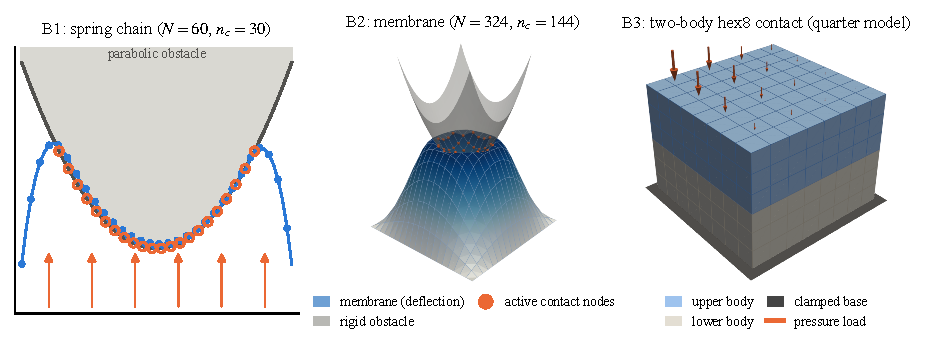
\includegraphics[width=\textwidth]{fig_geometry.pdf}
\caption{Benchmark problems, drawn from the problem definitions used in the experiments with the PyVista tools of the FEA package. B1: 60-node spring chain above a parabolic rigid obstacle; every second node can touch it (circles: active contact nodes for one query). B2: clamped membrane on an $18\times18$ interior grid, pushed by a Gaussian load against a curved rigid obstacle over a central $12\times12$ contact patch (membrane colored by deflection, active contact nodes in orange). B3: quarter model of two stacked linear-elastic hexahedral blocks with a matched node-to-node interface, a Gaussian pressure on the top face, a clamped base and symmetry planes; the mesh shown ($8\times8$ elements, $3+3$ layers) is smaller than the meshes of the experiments.}
\label{fig:geometry}
\end{figure}

\begin{longtable}[]{@{}
  >{\raggedright\arraybackslash}p{(\columnwidth - 10\tabcolsep) * \real{0.1667}}
  >{\raggedright\arraybackslash}p{(\columnwidth - 10\tabcolsep) * \real{0.1667}}
  >{\raggedright\arraybackslash}p{(\columnwidth - 10\tabcolsep) * \real{0.1667}}
  >{\raggedright\arraybackslash}p{(\columnwidth - 10\tabcolsep) * \real{0.1667}}
  >{\raggedright\arraybackslash}p{(\columnwidth - 10\tabcolsep) * \real{0.1667}}
  >{\raggedright\arraybackslash}p{(\columnwidth - 10\tabcolsep) * \real{0.1667}}@{}}
\toprule
Benchmark & Spatial Dim. & Full-Order \(N\) & Contact Rows \(n_c\) & Stiffness \(K(\mu)\) & Primary Purpose \\
\midrule
\endhead
\textbf{B1 (Spring Chain)} \cite{pawar2025efficient} & 1D & \(60\) & \(30\) & Constant & Silent SVD failure \& rank-repair overhead \\
\textbf{B2 (Obstacle Membrane)} \cite{benaceur2020reduced} & 2D & \(324\) & \(144\) & Constant & Five-basis comparison \& break-even size sweep \\
\textbf{B3 (3D Two-Body Contact)} \cite{franceschini2022block, koller2021hyper} & 3D & \(16\,653\) & \(441\) & Parametrized \(K(\mu)\) & Large-scale wall-clock speedup \& 3D effectivity \\
\bottomrule
\end{longtable}

\hypertarget{experimental-campaign-e1e6}{%
\subsection{Experimental Campaign (E1--E5)}\label{experimental-campaign-e1e6}}

\begin{itemize}
\item
  \textbf{Experiment E1: Silent Failure Audit (B1, B2)}
  Using identical primal POD bases \(V_0\) and signed-SVD and NMF dual bases \(U\) of matched dimension \(r_\lambda \in \{4, 8, 12, 16, 20\}\), we log the reduced KKT residual \(\Vert R_{\text{red}}(u_r, \lambda_r)\Vert_\infty\) alongside the true relative energy-norm error \(\Vert u - \tilde{u}\Vert_K / \Vert u\Vert_K\), the four estimator terms \((\eta_{\text{eq}}, \eta_{\text{sign}}, \eta_{\text{gap}}, \eta_{\text{comp}})\) \cite{hild2007residual, banz2024generic, banz2026posteriori}, and the online admissibility indicator \(\eta_{\text{adm}}\). This experiment tests whether \(\eta_{\text{adm}}\) flags every case where \(\Vert R_{\text{red}}\Vert_\infty \le 10^{-12}\) masks substantial error in the lifted solution.
\item
  \textbf{Experiment E2: Bound Effectivity and Extrapolation Stress Test (B1, B2, B3)}
  We evaluate the upper bound from Theorem~\ref{thm:bound} and compute the \textbf{effectivity index} \cite{hild2007residual, zhang2014duality, fontana2024guaranteed}
  \begin{equation}\label{eq:eff}\begin{aligned}
  \theta_{\text{eff}}(\mu) &:= \frac{\eta_{\text{bound}}(\mu)}{\Vert u(\mu) - \tilde{u}(\mu)\Vert_K}, \qquad \eta_{\text{bound}}(\mu) := \left( \eta_{\text{eq}}^2 + 2\,\eta_{\text{comp}} + 2\,\Vert \lambda\Vert_2\,\eta_{\text{gap}} \right)^{1/2}, \\
  \eta_{\text{bound}}^{C}(\mu) &:= \left( \eta_{\text{eq}}^2 + 2\,\eta_{\text{comp}} + 2\,C_\lambda\,\eta_{\text{gap}} \right)^{1/2},
  \end{aligned}\end{equation}
  on two kinds of test sets:

  \begin{enumerate}
  \def\labelenumi{\arabic{enumi}.}
  \tightlist
  \item
    \emph{In-range test queries} drawn from the training range of the parameters (B1, B2, B3);
  \item
    \emph{Load-magnitude extrapolation} on B3 (\(P\) between \(1.3\) and \(2.0\) times the training maximum), expanding the active contact set beyond the training snapshots \cite{benaceur2020reduced}.
  \end{enumerate}
  Out-of-range queries on B1 and B2 (loads, obstacle shape and indenter position, including contact-patch translation) are reported separately below, and an in-sample validation set was not run.
\item
  \textbf{Experiment E3: Comparative Five-Basis Benchmark (B1, B2)}
  On identical snapshot matrices \((U_{\text{snap}}, \Lambda_{\text{snap}})\), we construct and compare all five dual-basis strategies from Section 4.1---\textbf{SVD+Repair} \cite{leberre2022condition}, \textbf{NMF} \cite{balajewicz2016projection}, \textbf{CPG} \cite{benaceur2020reduced}, \textbf{gIS} \cite{sambataro2026model, kollepara2024sparse}, and \textbf{RID} \cite{fauque2018hybrid, leberre2022condition}---across dual dimensions \(r_\lambda \in \{4, 8, 12, 16, 24\}\). Each method is evaluated along five Pareto axes:

  \begin{enumerate}
  \def\labelenumi{\arabic{enumi}.}
  \tightlist
  \item
    Lifted energy-norm displacement error and multiplier \(\ell_2\)-error;
  \item
    Online admissibility violation \(\eta_{\text{adm}}\);
  \item
    Primal rank-repair enrichment \(r_{\text{rep}}\) required to bring \(\text{cond}(B_r K_r^{-1} B_r^T)\) to at most \(10^6\) (reached in all cases except three B1 entries, see the discussion of Algorithm~\ref{alg:repair}) \cite{leberre2022condition};
  \item
    Active-set iteration count \(k_{\text{ROM}}\) and online wall-clock time;
  \item
    Offline basis construction wall-clock time.
  \end{enumerate}
\item
  \textbf{Experiment E4: Break-Even Cost Model Validation (B1, B2, B3)}
  We measure single-thread wall-clock execution times as functions of the enriched primal dimension \(r_u = r_{u,0} + r_{\text{rep}}\), active contact size \(m_{\text{act}}\), and mesh size \(N\) \cite{franceschini2022block, leberre2022condition, pawar2025efficient}. Measured speedup curves \(S_{\text{meas}} = t_{\text{FOM}} / t_{\text{ROM}}\) are plotted against the theoretical predictions \(S_{\text{pred}} = \mathcal{C}_{\text{FOM}} / \mathcal{C}_{\text{ROM}}\) from Equations~\eqref{eq:cfom}--\eqref{eq:crom} for the constant-\(K\) and parameter-varying-\(K\) cost models. The per-basis comparison covers B1 and B2, and the size sweeps cover the membrane (\(N = 25\)--\(2304\)) and B3 (\(N = 24\)--\(16\,653\)); B1 has a fixed size and is not swept. Break-even is the size from which the speedup stays above one.
\item
  \textbf{Experiment E5: Admissibility Screening on Large-Scale 3D Contact (B3)}
  On the 3D two-body contact model (\(N = 16\,653\), \(n_c = 441\)) \cite{franceschini2022block, koller2021hyper}, we deploy NMF and CPG dual bases (\(r_\lambda \in \{8, 16\}\)) with the online admissibility screening \(\eta_{\text{adm}} \le \tau_{\text{adm}}\) \cite{dabaghi2020posteriori}, with \(\tau_{\text{adm}}\) calibrated on 25 validation queries and tested on 25 in-range and 25 load-extrapolated queries, and a fallback to the full-order solve whenever \(\eta_{\text{adm}} > \tau_{\text{adm}}\).
\end{itemize}

An extension to time-dependent contact dynamics was considered as a further experiment but was not performed in the present study; it is listed as future work.

\hypertarget{quantitative-evaluation-metrics-and-acceptance-criteria}{%
\subsection{Quantitative Evaluation Metrics and Acceptance Criteria}\label{quantitative-evaluation-metrics-and-acceptance-criteria}}

To ensure objective assessment across all benchmarks, we predefine four quantitative validation metrics:
\begin{enumerate}
\tightlist
\item \textbf{Admissibility Detection Recall (Zero False Negatives):} A test query is classified as a silent failure when the projected KKT residual \(\Vert R_{\text{red}}\Vert_\infty\) is below \(10^{-12}\) while the relative energy-norm error exceeds \(5\%\). The criterion is satisfied when the calibrated indicator rejects every such query, that is, \(\eta_{\text{adm}} > \tau_{\text{adm}}\). \emph{Scope:} \(\tau_{\text{adm}}\) is calibrated per (basis, \(r_\lambda\)) on a held-out validation set as \(0.9\) times the smallest indicator value among validation silent failures and then scored on separate test queries. The criterion is therefore an empirical, finite-sample statement, not a guarantee, and it cannot be evaluated when the validation set contains no silent failure.
\item \textbf{Effectivity Sharpness:} The effectivity index \(\theta_{\text{eff}}\) of the bound \(\eta_{\text{bound}}\) in Eq.~\eqref{eq:eff} lies within \([1, 10]\) on at least \(90\%\) of the test queries whose relative energy error exceeds the \(5\%\) tolerance, that is, of the errors that the screening must detect. The bound is evaluated with the exact multiplier norm of the full-order solution, which is a validation quantity; the variant \(\eta_{\text{bound}}^{C}\) with the offline constant \(C_\lambda\), which is usable online, is reported alongside \cite{hild2007residual, benaceur2020reduced, fontana2024guaranteed}. \emph{Scope:} over all queries the effectivity grows like \(\text{err}^{-1/2}\) as errors shrink, so the all-query share is reported as a diagnostic only.
\item \textbf{Monotonic Error Correlation:} The Spearman rank correlation between \(\eta_{\text{bound}}\) and the true energy-norm error \(\Vert u - \tilde{u}\Vert_K\) exceeds \(0.90\) across all dual bases and reduced dimensions. \emph{Scope:} the minimum correlation across all basis--dimension combinations is reported as the conservative measure, together with the median; the correlation is computed over the test queries of each entry.
\item \textbf{Cost Crossover Accuracy:} The predicted break-even threshold \(\mathcal{C}_{\text{ROM}} = \mathcal{C}_{\text{FOM}}\) matches the measured wall-clock break-even point within a factor of \(2\). \emph{Scope:} evaluated on the benchmarks with a size sweep (B2, B3); B1 has a fixed size.
\end{enumerate}

\hypertarget{results-and-acceptance-outcome}{%
\subsection{Results and Acceptance Outcome}\label{results-and-acceptance-outcome}}

The criteria were scored on B1 (spring chain) and B2 (membrane) for the five dual bases with rank repair, \(r_\lambda \in \{4,8,12,16,24\}\), using 40 test and 40 validation queries (seed 42). Theorem~\ref{thm:bound} (\(\eta_{\text{bound}} \ge\) true energy error) held on every test query. Criterion 4 uses the E4 break-even sweeps on B2 and B3, and E5 on B3 is reported separately. The outcomes are mixed and are reported as obtained, without tuning. Table~\ref{tab:e3} gives the comparative assessment of the five bases (experiment E3) on which the criteria are scored. Although the signed SVD basis has the lowest offline construction cost, it produces substantial errors in the reconstructed displacement field and negative contact multipliers, with energy-norm errors of order one. NMF and CPG reach similar accuracy; NMF is about ten times more expensive to build (0.12--0.15\,s against 0.011--0.015\,s), and CPG needs more active-set iterations on B1 (15 against 8). The gIS strategy provides an inexpensive non-negative basis but has larger displacement errors than NMF and CPG at the tested dimension (energy error 0.07 on B1 and 0.24 on B2) and needs six repair vectors. RID achieves the smallest displacement errors in several configurations; this is accompanied by a larger effective dual dimension (23 and 98 dual rows for a nominal 16), 3 and 78 repair vectors, a large multiplier error on B1 (0.87) and the slowest online solve on B2 (1.15\,ms). The results vary with the dual dimension, and only \(r_\lambda=16\) is shown.

\begin{longtable}{@{}>{\raggedright\arraybackslash}p{0.18\textwidth}>{\raggedright\arraybackslash}p{0.36\textwidth}>{\raggedright\arraybackslash}p{0.36\textwidth}@{}}
\toprule
Criterion & B1 & B2 \\
\midrule
\endhead
1. Zero false negatives (calibrated \(\tau_{\text{adm}}\), pooled over \(r_\lambda\)) & Met only by CPG (0/10) and by RID with the consistent indicator \(\eta_{\text{adm,v2}}\) (0/108). Missed with Eq.~\eqref{eq:eta-adm}: SVD 5/200 (1/200 with \(\eta_{\text{adm,v2}}\)), NMF 1/7, GIS 2/119, RID 3/108. Several NMF, CPG and RID entries have no validation silent failure, so no threshold exists. & Met by SVD (0/200), NMF (0/78) and GIS (0/188). CPG misses 1/115. RID has no silent failures (not evaluable). False-alarm rates on accurate queries are high: NMF 37--41\%, CPG 55--58\%, GIS 95--100\%. \\
2. \(\theta_{\text{eff}} \in [1,10]\) on \(\ge 90\%\) of queries above the 5\% tolerance & Met: SVD and NMF 100\% (200 and 7 queries). & Met: SVD and NMF 100\% (200 and 78 queries). \\
3. Spearman \(> 0.90\) (minimum over \(r_\lambda\); median in brackets) & Met by SVD 0.974 (0.978) and GIS 0.993 (0.996). Not met: NMF 0.515 (0.646), CPG 0.609 (0.686), RID \(-0.637\) (0.995). & Met by SVD 0.992 (0.995) and GIS 0.953 (0.994). Not met: NMF 0.486 (0.682), CPG 0.283 (0.494), RID 0.811 (0.979). \\
4. Break-even within a factor 2 & Not evaluated (fixed size, no sweep). & Membrane sweep, \(N = 25\)--\(2304\): predicted vs.\ measured \(N^*\) is 119 vs.\ 154 (ratio 0.78) in the affine regime and 64 vs.\ 37 (ratio 1.72) when \(K\) varies. Met in both. \textbf{B3 sweep} (\(N = 24\)--\(16653\)): constant \(K\) 779 vs.\ 1006 (ratio 0.77), met. Varying \(K\): 55 vs.\ 86 (ratio 0.64), met, but the measured speedup is not monotone below \(N = 105\) and the crossover rests on one point, so this is weak evidence. \\
\bottomrule
\end{longtable}

\emph{How to read the table.} Entries of criterion 1 are missed silent failures over silent failures, pooled over the five dual dimensions and scored on the test queries with the threshold calibrated on the 40 validation queries (seed 42). ``No threshold exists'' means that, for that basis and dual dimension, the validation set contained no silent failure, so the rule $\tau_{\mathrm{adm}} = 0.9\min(\eta_{\mathrm{adm}})$ is undefined; such entries are left out of the counts. A count of 0 in the table is therefore a statement about the calibrated entries only, and the denominators differ between bases. ``Not evaluable'' means the test set itself contained no silent failure for that basis. Section~\ref{results-and-acceptance-outcome} gives the threshold calibration study that quantifies these effects with more seeds and validation queries.

\begin{table}[htbp]
\centering
\footnotesize
\caption{Head-to-head comparison of the five dual bases (experiment E3) at nominal dual dimension $r_\lambda=16$ with rank repair, median over 40 test queries, seed 42. $r_\lambda^{\mathrm{eff}}$: dual dimension actually used (RID retains extra contact rows); $r_{\mathrm{rep}}$: primal vectors added by rank repair; $\varepsilon_E$, $\varepsilon_\lambda$: median relative energy-norm and multiplier errors; $\min\tilde\lambda$: smallest lifted multiplier over the test queries; $k_{\mathrm{ROM}}$: median active-set iterations; $t_{\mathrm{on}}$: median online time per query; $t_{\mathrm{off}}$: offline construction time.}
\label{tab:e3}
\begin{tabular}{@{}llrrrrrrrr@{}}
\toprule
 & Basis & $r_\lambda^{\mathrm{eff}}$ & $r_{\mathrm{rep}}$ & $\varepsilon_E$ & $\varepsilon_\lambda$ & $\min\tilde\lambda$ & $k_{\mathrm{ROM}}$ & $t_{\mathrm{on}}$ (ms) & $t_{\mathrm{off}}$ (s) \\
\midrule
B1 & SVD & 16 & 0 & 0.97 & 1.4 & $-1.6$ & 3 & 0.24 & 0.001 \\
 & NMF & 16 & 0 & $1.8\!\times\!10^{-3}$ & $9.2\!\times\!10^{-3}$ & 0 & 8 & 0.40 & 0.12 \\
 & CPG & 16 & 3 & $2.7\!\times\!10^{-3}$ & $9.3\!\times\!10^{-3}$ & 0 & 15 & 0.63 & 0.011 \\
 & gIS & 16 & 6 & 0.074 & 0.31 & 0 & 3 & 0.25 & 0.002 \\
 & RID & 23 & 3 & $6.3\!\times\!10^{-5}$ & 0.87 & 0 & 3 & 0.29 & 0.003 \\
\midrule
B2 & SVD & 16 & 0 & 1.0 & 1.8 & $-0.49$ & 3 & 0.31 & 0.002 \\
 & NMF & 16 & 0 & 0.036 & 0.13 & 0 & 6 & 0.46 & 0.15 \\
 & CPG & 16 & 0 & 0.046 & 0.15 & 0 & 7 & 0.48 & 0.015 \\
 & gIS & 16 & 6 & 0.24 & 2.0 & 0 & 5 & 0.43 & 0.003 \\
 & RID & 98 & 78 & $1.7\!\times\!10^{-3}$ & $1.0\!\times\!10^{-3}$ & 0 & 6 & 1.15 & 0.10 \\
\bottomrule
\end{tabular}
\end{table}

\begin{table}[htbp]
\centering
\small
\caption{Seed robustness of criteria 1 and 3 (seeds 42--46; entries are B1 / B2). Criterion 3: number of seeds, out of five, in which the minimum Spearman correlation over dual dimensions exceeds $0.9$, for the bound with the exact multiplier norm and for the online variant with the offline constant $C_\lambda$. Criterion 1: number of seeds in which no silent failure is missed (counted among seeds with at least one silent failure), for Eq.~\eqref{eq:eta-adm} and for the consistent indicator $\eta_{\mathrm{adm,v2}}$, with 40 and with 200 validation queries. RID had silent failures on B2 in only three of the five seeds, and many NMF, CPG and RID entries could not be calibrated (see text).}
\label{tab:robust}
\begin{tabular}{@{}lcccccc@{}}
\toprule
 & \multicolumn{2}{c}{Crit.~3} & \multicolumn{2}{c}{Crit.~1, 40 validation} & \multicolumn{2}{c}{Crit.~1, 200 validation} \\
\cmidrule(lr){2-3}\cmidrule(lr){4-5}\cmidrule(lr){6-7}
Basis & exact & $C_\lambda$ & Eq.~\eqref{eq:eta-adm} & $\eta_{\mathrm{adm,v2}}$ & Eq.~\eqref{eq:eta-adm} & $\eta_{\mathrm{adm,v2}}$ \\
\midrule
SVD & 5 / 5 & 5 / 5 & 3 / 4 & 2 / 4 & 5 / 5 & 5 / 5 \\
NMF & 0 / 0 & 0 / 3 & 3 / 1 & 3 / 2 & 5 / 3 & 5 / 5 \\
CPG & 0 / 0 & 0 / 0 & 3 / 3 & 4 / 3 & 5 / 4 & 5 / 5 \\
gIS & 2 / 5 & 2 / 5 & 0 / 1 & 0 / 1 & 3 / 3 & 4 / 4 \\
RID & 0 / 3 & 0 / 4 & 0 / 2 & 3 / 2 & 3 / 3 & 5 / 3 \\
\bottomrule
\end{tabular}
\end{table}

\paragraph{Threshold calibration study.}
To quantify how reliable the calibrated screen is, we repeated the E3 audit for eight seeds (42--49) on B1 and B2 with a pool of 200 validation queries and 100 test queries per seed. Smaller validation sets are random subsets of the pool (20 draws each), so the validation-size sweep needs no extra solves. Positives are silent failures (reduced KKT residual below $10^{-12}$, relative energy error above $5\%$) and negatives are accurate queries (error at most $5\%$), as in the main tables; counts are pooled over the five dual dimensions. Three threshold rules are compared for Eq.~\eqref{eq:eta-adm}. The \emph{$0.9\,\min$ rule} is the one used so far, $\tau_{\mathrm{adm}} = 0.9\min(\eta_{\mathrm{adm}})$ over validation silent failures; it is undefined when the validation set contains none. The \emph{relative rule} $\tau_{\mathrm{adm}} = 0.05\,\overline{\|u\|_K}$ (training mean) needs no validation data. The \emph{hybrid rule} takes the smaller of the two when the validation set contains a silent failure and the relative value otherwise, so it is always defined. Uncertainty is a $95\%$ percentile bootstrap interval \cite{efron1979bootstrap} resampling whole seeds, the independent units; intervals from pooled query counts would be too narrow because queries, dual dimensions and subsets are dependent.

\begin{table}[htbp]
\centering
\small
\caption{Detection of silent failures with Eq.~\eqref{eq:eta-adm}, 40 validation queries, eight seeds, five dual dimensions pooled; brackets are $95\%$ bootstrap intervals over seeds. Recall is the share of silent failures flagged; the false-alarm rate is the share of accurate queries flagged. ``Uncal.'' is the share of (seed, dual dimension) entries for which the $0.9\,\min$ rule has no threshold because the validation set holds no silent failure; the recall of that rule is computed over the remaining entries only. Signed SVD is omitted: it has no accurate queries and its recall is at least $0.99$.}
\label{tab:calibration}
\begin{tabular}{@{}llcccc@{}}
\toprule
 & & \multicolumn{2}{c}{$0.9\,\min$ rule} & \multicolumn{2}{c}{hybrid rule} \\
\cmidrule(lr){3-4}\cmidrule(lr){5-6}
Bench. & Basis & Recall & Uncal. & Recall & False-alarm rate \\
\midrule
B1 & NMF & 0.900 [0.84, 0.96] & 0.74 & 0.934 [0.90, 0.97] & 0.023 [0.02, 0.03] \\
 & CPG & 0.909 [0.88, 0.94] & 0.46 & 0.959 [0.93, 0.98] & 0.043 [0.04, 0.05] \\
 & gIS & 0.967 [0.96, 0.97] & 0.03 & 1.000 [1.00, 1.00] & 0.020 [0.01, 0.03] \\
 & RID & 0.982 [0.98, 0.99] & 0.36 & 0.993 [0.99, 1.00] & 0.019 [0.00, 0.05] \\
\midrule
B2 & NMF & 0.971 [0.96, 0.98] & 0.00 & 0.971 [0.96, 0.98] & 0.306 [0.28, 0.33] \\
 & CPG & 0.975 [0.97, 0.98] & 0.00 & 0.975 [0.97, 0.98] & 0.529 [0.47, 0.59] \\
 & gIS & 0.981 [0.97, 0.99] & 0.00 & 0.982 [0.97, 0.99] & 0.517 [0.49, 0.55] \\
 & RID & 0.970 [0.95, 0.98] & 0.82 & 0.970 [0.95, 0.98] & 0.015 [0.00, 0.04] \\
\bottomrule
\end{tabular}

\end{table}

\begin{figure}[htbp]
\centering
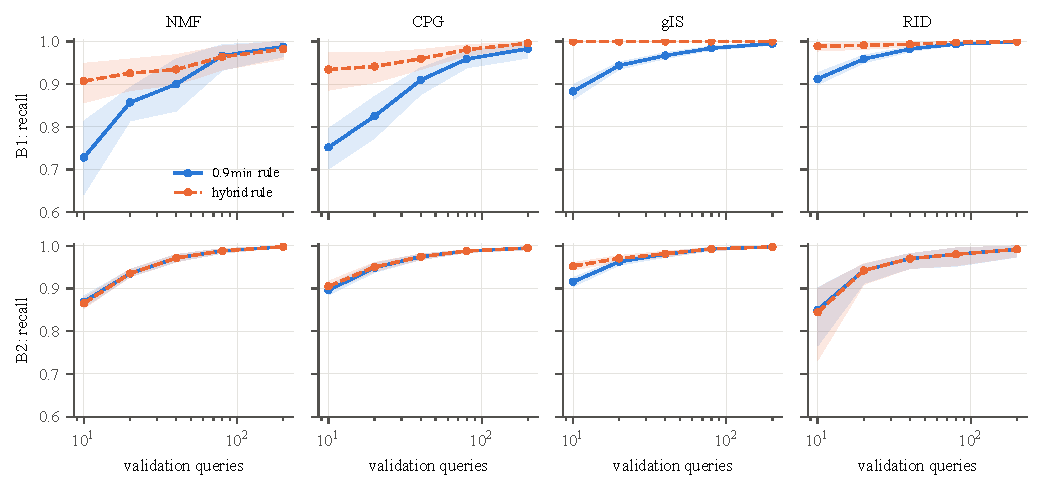
\includegraphics[width=\textwidth]{fig_calibration.pdf}
\caption{Recall of the calibrated screen, Eq.~\eqref{eq:eta-adm}, against the number of validation queries (eight seeds; bands are $95\%$ bootstrap intervals over seeds). The $0.9\,\min$ rule is scored on calibrated entries only, so it is optimistic when many entries are uncalibrated (Table~\ref{tab:calibration}, for example B1 NMF, 0.74).}
\label{fig:calibration}
\end{figure}

\paragraph{Threshold sensitivity, alternative rules and the cost of fallback.}
Figure~\ref{fig:thrsens} shows how the false-negative rate, the false-positive rate and the share of queries accepted by the ROM change with the threshold, written as $\tau_{\mathrm{adm}}/\tau_{\mathrm{rel}}$ with $\tau_{\mathrm{rel}}$ the relative threshold of the calibration study; counts are pooled over seeds and dual dimensions on the test sets. Figure~\ref{fig:tradeoff} plots the false-negative rate against the share of queries accepted, a trade-off curve of the receiver-operating-characteristic type \cite{fawcett2006introduction}. In both, a rate of silent failures that is not small makes the trade-off steep: on B1 NMF and CPG accept about $90\%$ of the queries before the first miss, whereas gIS and RID accept only about $40\%$ because their silent failures are numerous; on B2 a false-negative rate of $1\%$ requires sending about $65\%$ of the NMF queries, and more than $90\%$ of the gIS queries, to the full-order solver.

\begin{figure}[htbp]
\centering
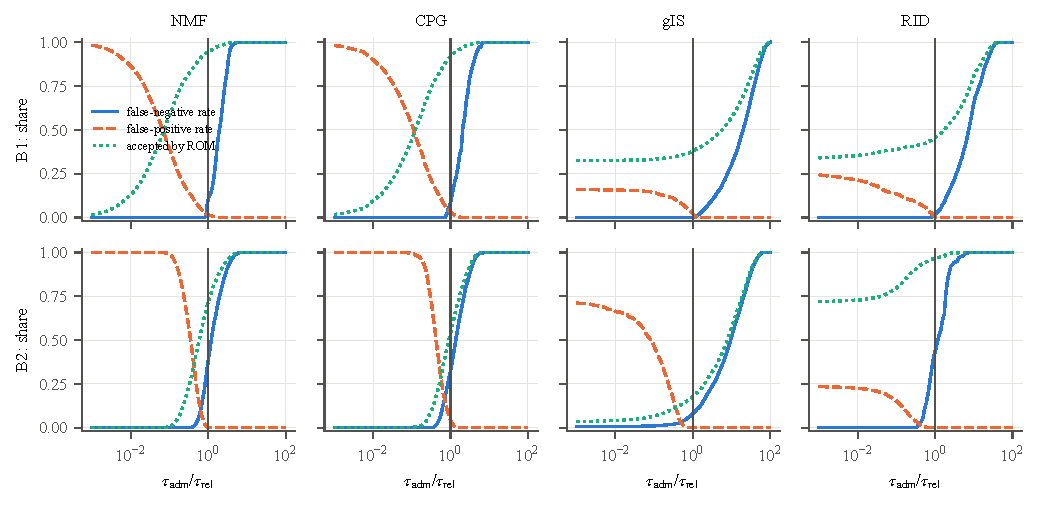
\includegraphics[width=\textwidth]{fig_threshold_sensitivity.pdf}
\caption{False-negative rate, false-positive rate and share of queries accepted by the ROM as functions of the threshold of Eq.~\eqref{eq:eta-adm}, relative to $\tau_{\mathrm{rel}}$ (vertical line). Eight seeds, five dual dimensions pooled, test sets.}
\label{fig:thrsens}
\end{figure}

\begin{figure}[htbp]
\centering
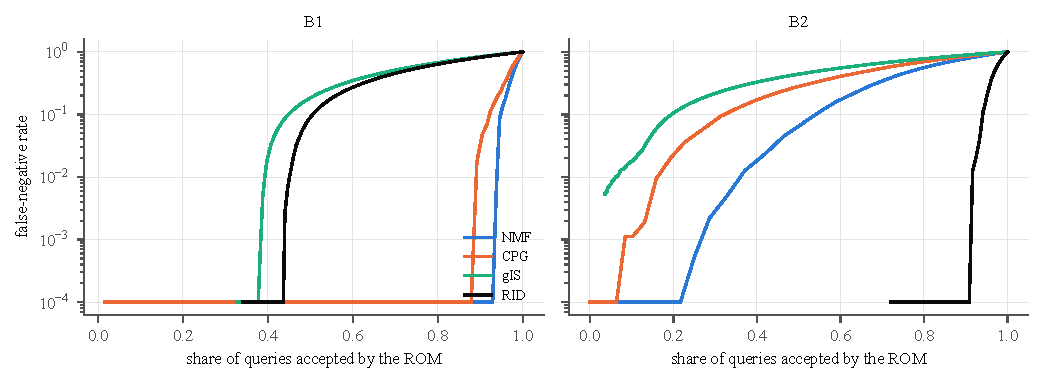
\includegraphics[width=\textwidth]{fig_tradeoff.pdf}
\caption{False-negative rate against the share of queries accepted by the ROM, obtained by sweeping the threshold of Eq.~\eqref{eq:eta-adm} (eight seeds, five dual dimensions pooled). The floor of the vertical axis is $10^{-4}$.}
\label{fig:tradeoff}
\end{figure}

Table~\ref{tab:rules} compares five calibration rules on the validation queries (40 per seed). Besides the $0.9\,\min$ and hybrid rules, two percentile rules set $\tau_{\mathrm{adm}}$ to the 10th or 25th percentile of the indicator over the validation silent failures, which accepts a validation false-negative rate of about $10\%$ or $25\%$ in exchange for fewer false alarms, and a cost-optimal rule minimizes $20\,\mathrm{FN} + \mathrm{FP}$ on the validation set, that is, it prices a false acceptance at twenty needless fallbacks. All rules except the hybrid rule need at least one validation silent failure; the share of entries without one is given in parentheses.

\begin{table}[htbp]
\centering
\small
\caption{Recall / false-alarm rate on the test sets for five calibration rules with Eq.~\eqref{eq:eta-adm}, 40 validation queries, eight seeds, five dual dimensions pooled. Parentheses: share of entries for which the rule is undefined (no validation silent failure), which are excluded from recall and false-alarm rate. The percentile rules give recall close to $1 - q$ by construction.}
\label{tab:rules}
\begin{tabular}{@{}llccccc@{}}
\toprule
Bench. & Basis & $0.9\min$ & 10th pct. & 25th pct. & cost-optimal & hybrid \\
\midrule
B1 & NMF & 0.90 / 0.10 (0.74) & 0.81 / 0.05 (0.74) & 0.72 / 0.03 (0.74) & 0.94 / 0.10 (0.74) & 0.93 / 0.02 \\
 & CPG & 0.91 / 0.07 (0.46) & 0.80 / 0.04 (0.46) & 0.72 / 0.02 (0.46) & 0.93 / 0.08 (0.46) & 0.96 / 0.04 \\
 & gIS & 0.97 / 0.00 (0.03) & 0.86 / 0.00 (0.03) & 0.72 / 0.00 (0.03) & 1.00 / 0.07 (0.03) & 1.00 / 0.02 \\
 & RID & 0.98 / 0.10 (0.36) & 0.87 / 0.03 (0.36) & 0.71 / 0.01 (0.36) & 1.00 / 0.21 (0.36) & 0.99 / 0.02 \\
\midrule
B2 & NMF & 0.97 / 0.31 & 0.86 / 0.11 & 0.72 / 0.05 & 0.97 / 0.28 & 0.97 / 0.31 \\
 & CPG & 0.97 / 0.53 & 0.87 / 0.24 & 0.72 / 0.13 & 0.97 / 0.51 & 0.97 / 0.53 \\
 & gIS & 0.98 / 0.52 & 0.89 / 0.01 & 0.74 / 0.00 & 0.99 / 0.62 & 0.98 / 0.52 \\
 & RID & 0.97 / 0.12 (0.82) & 0.89 / 0.05 (0.82) & 0.74 / 0.02 (0.82) & 0.98 / 0.12 (0.82) & 0.97 / 0.01 \\
\bottomrule
\end{tabular}

\end{table}

The percentile rules buy a lower false-alarm rate at a recall that falls by about the percentile (recall $0.71$--$0.89$ for the 10th and 25th), so they move along the trade-off curve and do not improve it. The cost-optimal rule behaves like the $0.9\,\min$ rule, with recall $0.94$--$1.00$ and a lower false-alarm rate in some cases (B2 NMF $0.28$ against $0.31$) and a higher one in others (B2 gIS $0.62$ against $0.52$, B1 RID $0.21$ against $0.10$). A single exception is worth noting: for gIS on B2 the 10th-percentile rule keeps recall at $0.89$ and cuts the false-alarm rate from $0.52$ to $0.01$. No rule removes the trade-off; the choice of rule is a choice of operating point, and for a deployment it should be made with the cost of a missed failure against that of a fallback in view.

The false alarms and the true failures both send queries to the full-order solver, so the fallback share can erase the speedup. Table~\ref{tab:netspeed} combines the measured membrane speedups ($r_\lambda = 16$, Section~\ref{sec:basis_cost}) with the fallback share of the hybrid rule: the net speedup of a screened ROM that re-solves a fraction $f$ of the queries at full order is $1/(1/S + f)$, with the reduced solve always executed.

\begin{table}[htbp]
\centering
\small
\caption{Net speedup on the membrane with fallback. $f$: share of test queries flagged by the hybrid rule (40 validation queries, eight seeds, five dual dimensions pooled) and sent to the full-order solver; $S$: measured speedup of the unscreened ROM at $r_\lambda = 16$ (single-run sweep). Net speedup is $1/(1/S + f)$.}
\label{tab:netspeed}
\begin{tabular}{@{}lccccc@{}}
\toprule
Basis & fallback share $f$ & $S$ (const. $K$) & net & $S$ (varying $K$) & net \\
\midrule
NMF & 0.60 & 1.69 & 0.84 & 5.3 & 1.3 \\
CPG & 0.83 & 1.56 & 0.68 & 5.1 & 1.0 \\
gIS & 0.94 & 1.75 & 0.66 & 5.5 & 0.9 \\
RID & 0.07 & 0.76 & 0.72 & 2.2 & 1.9 \\
\bottomrule
\end{tabular}

\end{table}

\paragraph{Out-of-range queries and contact-patch translation.}
The calibration and comparison studies query the reduced models inside the training box. We therefore also queried the five bases ($r_\lambda = 16$, rank repair, five seeds, 40 queries per set and seed) outside it: loads $1.3$ to $2$ times the training maximum on both benchmarks, a steeper obstacle on B1 (curvature $1.25$ to $1.7$ times the training maximum), and an indenter centre outside the training box on B2, which moves the contact patch (each coordinate in $[0.20, 0.30]$ or $[0.70, 0.80]$ against $[0.35, 0.65]$ in training). The screening indicator uses the hybrid threshold calibrated on the in-range validation queries. Table~\ref{tab:extrap} gives the share of queries above $5\%$ error, the missed silent failures among the silent failures, and the validity of the online bound with the offline constant $C_\lambda$.

\begin{table}[htbp]
\centering
\footnotesize
\setlength{\tabcolsep}{3pt}
\caption{Out-of-range queries. Cells: share of queries above $5\%$ error in \% (silent failures missed by the screening indicator / silent failures), five seeds pooled (200 queries per cell). The screening indicator uses the hybrid threshold of Eq.~\eqref{eq:eta-adm} calibrated on the 40 in-range validation queries of each seed. Last column: smallest share, over the five bases, of queries on which the bound with the offline constant $C_\lambda$ is at least the true error; the bound with the exact multiplier norm held on every query in every set.}
\label{tab:extrap}
\begin{tabular}{@{}llcccccc@{}}
\toprule
Bench. & Query set & SVD & NMF & CPG & gIS & RID & $C_\lambda$ bound valid (\%) \\
\midrule
B1 & in range & 100 (0/200) & 0 (0/0) & 0 (0/0) & 52 (0/103) & 34 (1/68) & 100.0 \\
 & load $\times$1.3--2 & 100 (0/200) & 26 (0/53) & 37 (0/74) & 100 (0/200) & 70 (20/140) & 98.5 \\
 & steeper obstacle & 100 (0/200) & 0 (0/0) & 1 (0/2) & 0 (0/0) & 16 (0/32) & 100.0 \\
\midrule
B2 & in range & 100 (0/200) & 26 (6/51) & 44 (0/89) & 83 (7/166) & 0 (0/0) & 100.0 \\
 & load $\times$1.3--2 & 100 (0/200) & 99 (0/198) & 100 (0/200) & 100 (0/200) & 45 (78/90) & 100.0 \\
 & centre outside & 100 (0/200) & 96 (2/192) & 96 (2/192) & 96 (2/191) & 0 (0/0) & 96.5 \\
\bottomrule
\end{tabular}

\end{table}

\paragraph{Mesh-size study.}
To see whether the findings depend on the mesh, we repeated the audit on five mesh sizes of B1 (chain length $30$ to $480$ with $n_c = N/2$) and B2 (membrane grid $12$ to $40$, $N = 144$ to $1600$, with the contact sub-grid and the load scaled as in the break-even sweep), with three seeds, 40 test queries, the dual dimension fixed at $r_\lambda = 16$ and the primal dimension at $20$ (Table~\ref{tab:mesh}). The speedup is that of the unscreened ROM against the full-order solver in the constant-stiffness regime. We did not repeat this study on B3, whose break-even sweep (Table~\ref{tab:timing}) is the only mesh study there.

\begin{table}[htbp]
\centering
\footnotesize
\setlength{\tabcolsep}{3pt}
\caption{Mesh-size study (three seeds, 40 test queries each, $r_\lambda = 16$): share of queries above $5\%$ error for SVD, NMF (with median error in brackets) and gIS, and the measured speedup $S$ of the unscreened ROM for NMF and gIS (constant stiffness).}
\label{tab:mesh}
\begin{tabular}{@{}lrrcccrr@{}}
\toprule
Bench. & $N$ & $n_c$ & SVD $>5\%$ & NMF $>5\%$ (med.) & gIS $>5\%$ & $S$ NMF & $S$ gIS \\
\midrule
B1 & 30 & 15 & 100 & 0 (0.00013) & 0 & 0.21 & 0.45 \\
 & 60 & 30 & 100 & 0 (0.002) & 51 & 0.33 & 0.52 \\
 & 120 & 60 & 100 & 0 (0.0034) & 82 & 0.47 & 0.75 \\
 & 240 & 120 & 100 & 0 (0.005) & 88 & 1.12 & 1.33 \\
 & 480 & 240 & 100 & 0 (0.0042) & 89 & 2.91 & 3.40 \\
\midrule
B2 & 144 & 64 & 100 & 12 (0.028) & 69 & 0.81 & 0.60 \\
 & 324 & 144 & 100 & 25 (0.037) & 83 & 1.83 & 1.75 \\
 & 576 & 256 & 100 & 26 (0.038) & 90 & 4.10 & 4.22 \\
 & 1024 & 441 & 100 & 29 (0.039) & 96 & 14.09 & 13.38 \\
 & 1600 & 729 & 100 & 32 (0.04) & 98 & 45.41 & 44.14 \\
\bottomrule
\end{tabular}

\end{table}

\paragraph{Ablation of the framework components.}
To isolate what each component contributes, we compared four configurations on B1 and B2 (constant stiffness; five seeds with 40 test and 40 validation queries each, so 200 queries per row; primal dimension 20, dual dimension 16). (i)~A \emph{primal-only} ROM reduces the displacements and keeps all $n_c$ multipliers. (ii)~A \emph{primal--dual} ROM with a dual basis (signed SVD, NMF, CPG or gIS) and no primal repair. (iii)~The same with supremizer rank repair. (iv)~Configuration (iii) with the interface-based screening indicator of Eq.~\eqref{eq:eta-adm}, the hybrid threshold calibrated on the validation queries, and a full-order re-solve of every flagged query; its error and speedup are those of the answers actually served. Table~\ref{tab:ablation} gives the results.

\begin{table}[htbp]
\centering
\footnotesize
\setlength{\tabcolsep}{2.5pt}
\caption{Ablation on B1 and B2 (200 queries per row). Median err.: median relative energy error of the served answer; $>5\%$: share of served answers above $5\%$ error; cond.: median condition number of the reduced Schur complement (infinite when singular); speedup: mean full-order time over mean time of the configuration (net of the fallback in the last variant, whose served errors are zero for the flagged queries); Fallback: share of queries re-solved at full order; Missed: accepted queries with error above $5\%$. Speedups come from one timing per query, and models that are identical (for example NMF with and without repair, where repair adds no vector) differ by up to about $10\%$.}
\label{tab:ablation}
\begin{tabular}{@{}lllrrrrrrrr@{}}
\toprule
Bench. & Variant & Basis & Median err. & $>5\%$ (\%) & cond. & $r_u$ & kFLOPs & Speedup & Fallback & Missed \\
\midrule
B1 & Primal only & -- & 0.0023 & 44 & $\infty$ & 20 & 131 & 0.04 & -- & -- \\
 & Primal--dual, no repair & SVD & 0.95 & 100 & 2e1 & 20 & 29 & 0.65 & -- & -- \\
 & Primal--dual, repair & SVD & 0.95 & 100 & 2e1 & 20 & 29 & 0.58 & -- & -- \\
 & Repair + screen + fallback & SVD & 0 & 0 & 2e1 & 20 & 29 & 0.36 & 1.00 & 0 \\
 & Primal--dual, no repair & NMF & 0.0021 & 0 & 1e5 & 20 & 32 & 0.37 & -- & -- \\
 & Primal--dual, repair & NMF & 0.0021 & 0 & 1e5 & 20 & 32 & 0.37 & -- & -- \\
 & Repair + screen + fallback & NMF & 0.0021 & 0 & 1e5 & 20 & 32 & 0.36 & 0.00 & 0 \\
 & Primal--dual, no repair & CPG & 0.0038 & 0 & 1e7 & 20 & 29 & 0.24 & -- & -- \\
 & Primal--dual, repair & CPG & 0.0038 & 0 & 1e7 & 23 & 36 & 0.24 & -- & -- \\
 & Repair + screen + fallback & CPG & 0.0038 & 0 & 1e7 & 23 & 36 & 0.24 & 0.00 & 0 \\
 & Primal--dual, no repair & gIS & 0.18 & 68 & $\infty$ & 20 & 61 & 0.07 & -- & -- \\
 & Primal--dual, repair & gIS & 0.061 & 52 & 1e3 & 26 & 52 & 0.56 & -- & -- \\
 & Repair + screen + fallback & gIS & 0 & 0 & 1e3 & 26 & 52 & 0.41 & 0.55 & 0 \\
\midrule
B2 & Primal only & -- & 0.031 & 11 & $\infty$ & 20 & 1615 & 0.01 & -- & -- \\
 & Primal--dual, no repair & SVD & 0.93 & 100 & 7e1 & 20 & 38 & 1.99 & -- & -- \\
 & Primal--dual, repair & SVD & 0.93 & 100 & 7e1 & 20 & 38 & 2.05 & -- & -- \\
 & Repair + screen + fallback & SVD & 0 & 0 & 7e1 & 20 & 38 & 0.66 & 1.00 & 0 \\
 & Primal--dual, no repair & NMF & 0.038 & 26 & 1e4 & 20 & 39 & 1.47 & -- & -- \\
 & Primal--dual, repair & NMF & 0.038 & 26 & 1e4 & 20 & 39 & 1.32 & -- & -- \\
 & Repair + screen + fallback & NMF & 0.022 & 3 & 1e4 & 20 & 39 & 0.89 & 0.39 & 6 \\
 & Primal--dual, no repair & CPG & 0.047 & 44 & 2e5 & 20 & 37 & 1.30 & -- & -- \\
 & Primal--dual, repair & CPG & 0.047 & 44 & 2e5 & 20 & 37 & 1.42 & -- & -- \\
 & Repair + screen + fallback & CPG & 0 & 0 & 2e5 & 20 & 37 & 0.65 & 0.83 & 0 \\
 & Primal--dual, no repair & gIS & 0.19 & 82 & $\infty$ & 20 & 41 & 0.56 & -- & -- \\
 & Primal--dual, repair & gIS & 0.19 & 83 & 1e5 & 23 & 49 & 1.42 & -- & -- \\
 & Repair + screen + fallback & gIS & 0 & 4 & 1e5 & 23 & 49 & 0.60 & 0.90 & 7 \\
\bottomrule
\end{tabular}

\end{table}

\paragraph{Comparison at matched effective dimension, cost and accuracy.}
Table~\ref{tab:e3} compares the bases at the same nominal $r_\lambda$, but the effective sizes differ: RID keeps all contact rows of the selected elements (23 rows on B1 and 98 on B2 at nominal 16), and gIS and RID need more primal rank-repair modes. We therefore audited all five bases on the same snapshots over $r_\lambda \in \{4,\dots,30\}$ (B1) and $\{4,\dots,60\}$ (B2), 100 test queries, with rank repair, and compare them on common axes (Tables~\ref{tab:matcheddim} and \ref{tab:matchedacc}, Figure~\ref{fig:basiscost}). The online cost is the FLOP count of Eq.~\eqref{eq:crom} for constant $K$ (reduced dense solves, reduced active-set iterations and the interface check), evaluated with the measured median iteration count and active-set size, and the measured median wall time of the reduced solve. A dual dimension above the number of training snapshots (60) is not available to the snapshot-span bases; NMF and CPG were still run up to 60.

Table~\ref{tab:effdim} lists, at nominal $r_\lambda = 16$, the effective dual dimension, the repair vectors, the enriched primal dimension and the offline and online costs of the five methods. The offline cost is that of the dual basis and the rank repair, measured in our implementation.

\begin{table}[htbp]
\centering
\small
\caption{Nominal and effective dimensions, primal repair, and offline and online cost of the five methods at nominal $r_\lambda = 16$ (100 test queries; online time is the median reduced-solve time).}
\label{tab:effdim}
\begin{tabular}{@{}llcccccrr@{}}
\toprule
Bench. & Method & Nominal $r_\lambda$ & Eff. $r_\lambda$ & Repair $r_{\mathrm{rep}}$ & $r_u$ & Offline (ms) & Online (kFLOPs) & Online ($\mu$s) \\
\midrule
B1 & SVD + repair & 16 & 16 & 0 & 20 & 1 & 29 & 358 \\
 & NMF & 16 & 16 & 0 & 20 & 143 & 33 & 637 \\
 & CPG & 16 & 16 & 3 & 23 & 26 & 36 & 959 \\
 & gIS & 16 & 16 & 6 & 26 & 5 & 52 & 354 \\
 & RID & 16 & 23 & 3 & 23 & 6 & 65 & 411 \\
\midrule
B2 & SVD + repair & 16 & 16 & 0 & 20 & 2 & 37 & 293 \\
 & NMF & 16 & 16 & 0 & 20 & 193 & 39 & 419 \\
 & CPG & 16 & 16 & 0 & 20 & 20 & 37 & 444 \\
 & gIS & 16 & 16 & 6 & 26 & 3 & 59 & 407 \\
 & RID & 16 & 98 & 78 & 98 & 174 & 4459 & 1023 \\
\bottomrule
\end{tabular}

\end{table}

\begin{table}[htbp]
\centering
\small
\caption{Median relative energy error at matched effective dual dimension $r_\lambda^{\mathrm{eff}}$, with the effective dual and enriched primal dimensions in parentheses. The entry nearest to the target within $25\%$ is used; ``n/a'' means the basis cannot be built at that size (RID on B2 keeps at least 61 rows). Signed SVD is the only basis whose error stays near one.}
\label{tab:matcheddim}
\begin{tabular}{@{}llccccc@{}}
\toprule
Bench. & $r_{\lambda}^{\mathrm{eff}}$ target & SVD & NMF & CPG & gIS & RID \\
\midrule
B1 & 16 & 0.95 (16, 20) & 0.0021 (16, 20) & 0.003 (16, 23) & 0.051 (16, 26) & 0.26 (16, 20) \\
 & 24 & 1.2 (24, 24) & 0.00093 (24, 27) & 0.0016 (24, 22) & 2.9e-06 (24, 27) & 0.00038 (23, 23) \\
\midrule
B2 & 16 & 0.97 (16, 20) & 0.038 (16, 20) & 0.054 (16, 20) & 0.24 (16, 26) & n/a \\
 & 60 & 0.98 (60, 60) & 0.017 (60, 63) & 0.033 (60, 61) & 0.013 (60, 60) & 0.025 (61, 61) \\
\bottomrule
\end{tabular}

\end{table}

\begin{table}[htbp]
\centering
\small
\caption{Cheapest entry whose median error is at most the target: effective dual / enriched primal dimension, online FLOPs per query (thousands, Eq.~\eqref{eq:crom}), measured reduced-solve time in $\mu$s. ``Not reached'' means no entry up to $r_\lambda = 30$ (B1) or $60$ (B2) attains the target.}
\label{tab:matchedacc}
\begin{tabular}{@{}llccccc@{}}
\toprule
Bench. & Median error & SVD & NMF & CPG & gIS & RID \\
\midrule
B1 & 5\% & not reached & 4/20, 8k, 379 & 4/20, 8k, 432 & 20/26, 75k, 444 & 23/23, 65k, 411 \\
 & 1\% & not reached & 8/20, 14k, 479 & 12/20, 21k, 786 & 20/26, 75k, 444 & 23/23, 65k, 411 \\
\midrule
B2 & 5\% & not reached & 12/20, 28k, 376 & 24/25, 80k, 615 & 48/48, 740k, 659 & 61/61, 1183k, 675 \\
 & 1\% & not reached & not reached & not reached & not reached & 82/82, 2732k, 862 \\
\bottomrule
\end{tabular}

\end{table}

\begin{figure}[htbp]
\centering
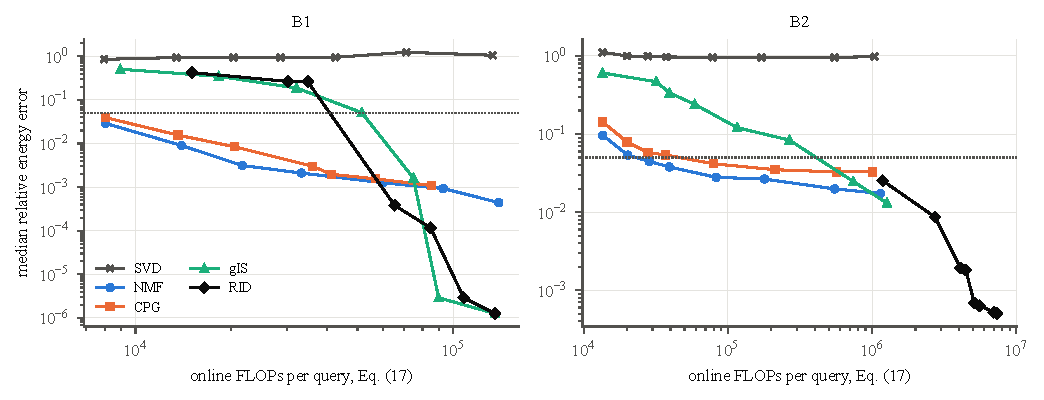
\includegraphics[width=\textwidth]{fig_basis_cost.pdf}
\caption{Median relative energy error against online FLOPs per query for the five bases, each point one nominal dual dimension (with rank repair). The dotted line is the $5\%$ silent-failure level. RID moves right quickly because its effective dual dimension and rank-repair modes grow with the nominal value.}
\label{fig:basiscost}
\end{figure}

\paragraph{Repeated timings and variability.}
The break-even sizes of Section~\ref{sec:basis_cost} come from single-thread wall-clock times, so we repeated the membrane (B2) and two-body (B3) size sweeps with ten timing repeats per query and ten queries per size, keeping every raw repeat. Point estimates use the estimator of the main tables (minimum over repeats, median over queries). Intervals are $95\%$ percentile bootstrap intervals that resample queries and repeats; for the break-even size $N^*$ every size is resampled independently and $N^*$ is recomputed. The measurement noise is moderate: the coefficient of variation across repeats of one query is $0.02$--$0.21$ over all sizes and solvers (Table~\ref{tab:timing}), and the spread between queries is larger, up to about $50\%$ for the reduced solve at some sizes, because the iteration counts differ.

\begin{table}[htbp]
\centering
\small
\caption{Predicted and measured break-even sizes $N^*$ and the speedup at the largest size (B2: $N = 2304$; B3: $N = 16\,653$), with $95\%$ bootstrap intervals. $N^*_{\mathrm{E4}}$ is the value of the earlier single-run sweep used in the other tables, $N^*_{\mathrm{meas}}$ the value of the ten-repeat run. pred/meas is $N^*_{\mathrm{pred}}/N^*_{\mathrm{meas}}$. $^{*}$: $N^*$ is defined in only $65\%$ (B2) and $79\%$ (B3) of the bootstrap resamples, because in the others the speedup exceeds one over the whole range or does not stay above one; the interval is conditional on that.}
\label{tab:timing}
\begin{tabular}{@{}llccccrr@{}}
\toprule
 & Regime & $N^*_{\mathrm{pred}}$ & $N^*_{\mathrm{E4}}$ & $N^*_{\mathrm{meas}}$ [95\%] & pred/meas & $S_{\mathrm{pred}}$ & $S_{\mathrm{meas}}$ [95\%] \\
\midrule
B2 & constant $K$ & 119 & 154 & 143 [98, 164] & 0.83 & 1730 & 179 [74, 265] \\
 & varying $K$ & 64 & 37 & 32 [28, 35]$^{*}$ & 1.97 & 628 & 287 [232, 328] \\
\multicolumn{8}{@{}l}{\scriptsize B2: CV across repeats 0.05--0.17 (reduced), 0.05--0.16 (full-order, constant $K$), 0.03--0.14 (full-order, varying $K$)} \\
\midrule
B3 & constant $K$ & 779 & 1006 & 722 [644, 937] & 1.08 & 730 & 48 [39, 62] \\
 & varying $K$ & 55 & 86 & 67 [64, 72]$^{*}$ & 0.82 & 1138 & 411 [396, 475] \\
\multicolumn{8}{@{}l}{\scriptsize B3: CV across repeats 0.05--0.21 (reduced), 0.03--0.12 (full-order, constant $K$), 0.02--0.15 (full-order, varying $K$)} \\
\bottomrule
\end{tabular}

\end{table}

\begin{table}[htbp]
\centering
\small
\caption{Storage of the full-order sparse factorization and of the reduced dense model on the break-even sweeps (constant $K$; double-precision values, index arrays not counted). Full-order: stored entries of $L$ and $U$ from SuperLU (the factorization of the timing study, default column ordering) plus the dense $n_c\times n_c$ block $A=BK^{-1}B^T$. Reduced: $r_u^2+r_\lambda^2+n_c r_\lambda+n_c r_u$ with $r_\lambda=12$ and $r_u$ from the timing study (about $20$), and, in the last storage column, $N r_u$ more for the primal basis needed to reconstruct the full field. Meshes with $N<100$ are omitted. Fitted exponent of $\mathrm{nnz}(L+U)\propto N^{\alpha}$ for $N\ge 200$: $\alpha=1.35$ (B2), $1.59$ (B3).}
\label{tab:memory}
\begin{tabular}{@{}lrrrrrrrr@{}}
\toprule
 & & & fill & \multicolumn{3}{c}{storage (MiB)} & \multicolumn{2}{c}{ratio} \\
\cmidrule(lr){5-7}\cmidrule(lr){8-9}
Bench. & $N$ & $n_c$ & $\mathrm{nnz}(L{+}U)/\mathrm{nnz}(K)$ & full-order & reduced & reduced + lift & online & with lift \\
\midrule
B2 & 144 & 64 & 3.7 & 0.050 & 0.020 & 0.042 & 2.5 & 1.2 \\
 & 256 & 121 & 4.5 & 0.15 & 0.034 & 0.073 & 4.5 & 2.1 \\
 & 400 & 169 & 5.2 & 0.29 & 0.045 & 0.11 & 6.5 & 2.8 \\
 & 576 & 256 & 6.3 & 0.63 & 0.067 & 0.15 & 9.5 & 4.1 \\
 & 1024 & 441 & 7.5 & 1.77 & 0.11 & 0.27 & 15.8 & 6.6 \\
 & 1600 & 729 & 8.3 & 4.55 & 0.18 & 0.43 & 25.0 & 10.7 \\
 & 2304 & 1024 & 9.4 & 8.81 & 0.25 & 0.61 & 34.7 & 14.5 \\
\midrule
B3 & 105 & 9 & 1.7 & 0.040 & 0.007 & 0.024 & 5.9 & 1.7 \\
 & 200 & 16 & 1.8 & 0.10 & 0.008 & 0.041 & 11.8 & 2.5 \\
 & 325 & 25 & 2.0 & 0.20 & 0.010 & 0.060 & 19.4 & 3.3 \\
 & 665 & 49 & 2.5 & 0.56 & 0.020 & 0.15 & 27.6 & 3.7 \\
 & 1125 & 81 & 3.0 & 1.22 & 0.025 & 0.21 & 49.2 & 6.0 \\
 & 4329 & 169 & 6.0 & 11 & 0.045 & 0.71 & 251.2 & 16.2 \\
 & 9163 & 289 & 9.0 & 38 & 0.077 & 1.55 & 498.4 & 24.9 \\
 & 16653 & 441 & 13.5 & 109 & 0.12 & 2.78 & 943.3 & 39.1 \\
\bottomrule
\end{tabular}

\end{table}

\begin{itemize}
\tightlist
\item
  \textbf{Storage (Table~\ref{tab:memory}).} The reduced model needs less memory than the sparse factorization at every size in the table, and the gap grows with $N$, but the source of the gap differs between the benchmarks. On B3 the factor fill dominates: $\mathrm{nnz}(L+U)$ grows as $N^{1.59}$ and the fill ratio reaches $13.5$ at $N=16\,653$, where the full-order model stores about $109$\,MiB against $0.12$\,MiB for the online reduced model ($940$ times less) and $2.8$\,MiB when the primal basis is kept for reconstruction ($39$ times less). On B2 the factor grows only as $N^{1.35}$, and at $N=2304$ the dense $n_c\times n_c$ block holds $91\%$ of the full-order storage because roughly half of the nodes are contact candidates; the reduction there ($35$ times online, $14.5$ with the primal basis) comes mainly from $n_c$ being replaced by $r_\lambda$, not from avoiding fill. With the primal basis the advantage is moderate for all but the largest meshes, and at the smallest sizes ($N\approx 150$) it is a factor $1.2$--$1.7$. These counts use dense blocks for $A$, which a solver that never forms $BK^{-1}B^T$ would avoid, and they do not include the temporary memory used during factorization or the offline snapshot and basis matrices.
\item
  \textbf{Repeated timings (Table~\ref{tab:timing}).} The measured break-even sizes are broadly reproducible, but the model locates them only approximately and does not predict the speedup. For constant $K$ the ten-repeat sizes are $143$ [98, 164] (B2) and $722$ [644, 937] (B3), against $119$ and $779$ predicted. The earlier single-run value on B3 ($1006$) lies outside its interval, so run-to-run variability exceeds the bootstrap interval. For varying $K$ the sizes are $32$ [28, 35] (B2) and $67$ [64, 72] (B3), against $64$ and $55$ predicted. The B2 ratio of predicted to measured size is $1.97$ ($1.72$ in the single run) with an interval reaching about $2.3$, so agreement within a factor of two is marginal there; the varying-$K$ crossover on B3 is weakly determined because the measured speedup is not monotone at the smallest sizes. The speedup magnitudes are not reproduced. At the largest sizes the model predicts $1730$ against $179$ [74, 265] measured (B2, constant $K$), $628$ against $287$ (B2, varying $K$), $730$ against $48$ (B3, constant $K$) and $1138$ against $411$ (B3, varying $K$), and at small sizes the measured speedup exceeds the prediction. The model should therefore be used to locate the break-even size, to within roughly a factor of two of a noisy measurement, and not to predict the speedup.
\item
  \textbf{Out-of-range queries (Table~\ref{tab:extrap}).} All bases degrade outside the training box, and the screening indicator does not always detect the failures. A load $1.3$ to $2$ times the training maximum raises the share above $5\%$ on B1 from $0\%$ to $26\%$ (NMF), $37\%$ (CPG), $100\%$ (gIS) and $70\%$ (RID). On B2 the in-range shares of $26\%$ (NMF) and $44\%$ (CPG) rise to $99\%$ and $100\%$, and RID, which had no in-range failure, reaches $45\%$. Contact-patch translation on B2 affects NMF, CPG and gIS almost as strongly ($95$--$96\%$) but not RID ($0\%$ in the tested shifts). A steeper obstacle on B1 leaves NMF, CPG and gIS accurate ($0$--$1\%$) and affects RID ($16\%$). Where a threshold could be calibrated, the screening indicator flagged almost all failures (between $0$ of $200$ and $2$ of $192$ missed for NMF, CPG and gIS, excluding B2 in range). RID on B2 is the exception: its validation set contained no silent failure, so the hybrid rule used the relative default, and the indicator missed $78$ of the $90$ silent failures under load extrapolation ($20$ of $140$ on B1). This illustrates the limitation discussed in Section~\ref{sec:conclusion}: a screening threshold calibrated only in range may fail to detect failures outside it. The bound with the exact multiplier norm held on every query, whereas the online bound with the offline constant $C_\lambda$ fell below the true error on $1.5\%$ of the extrapolated queries on B1 (SVD, load) and on up to $3.5\%$ on B2 (RID, centre shift).
\item
  \textbf{Mesh size (Table~\ref{tab:mesh}).} At a fixed dual dimension, accuracy does not scale with the mesh, whereas the speedup grows with it. The silent-failure share increases with $N$ once the dual space no longer covers the contact set: for gIS on B1 from $0\%$ at $N = 30$ (where $n_c = 15 < r_\lambda$) to $89\%$ at $N = 480$, for gIS on B2 from $69\%$ to $97\%$, and for NMF on B2 from $12\%$ to $32\%$. NMF on B1 stays below $5\%$ at every size. The NMF speedup rises from $0.21$ at $N = 30$ to $2.9$ at $N = 480$ on B1 (break-even near $N = 220$ by interpolation) and from $0.81$ at $N = 144$ to $45$ at $N = 1600$ on B2 (break-even near $N = 180$, against $154$ in the sweep of Table~\ref{tab:timing}); the B1 value was not compared with the cost model. The bound with the exact multiplier norm holds at all meshes. The single value below $100\%$ (gIS at $N = 30$ on B1) occurs at a median error of the order of $10^{-15}$, which we attribute to rounding without having examined individual queries. The dual dimension should therefore grow with the contact set; this was not studied.
\item
  \textbf{Ablation (Table~\ref{tab:ablation}).} Dual reduction is what makes the ROM cheap, the dual basis decides whether it is admissible, rank repair affects solvability more than accuracy, and screening exchanges silent failures for fallbacks.
  \emph{Primal-only ROM.} Keeping all $n_c$ multipliers preserves primal feasibility and non-negativity by construction but is neither accurate nor cheap here. The reduced Schur complement is singular ($n_c > r_u$), and the median error is $0.0023$ (B1) and $0.031$ (B2), but $44\%$ (B1) and $11\%$ (B2) of the queries exceed $5\%$, with errors up to $692$ on B1 (we attribute this to the singular LCP but did not isolate the cause). The dense $n_c$-dimensional problem makes the ROM $25$ to $100$ times slower than the full-order solver.
  \emph{Dual basis.} The signed SVD basis fails on all queries ($100\%$ above $5\%$, median error $0.93$--$0.95$), whereas NMF and CPG give median errors of $0.002$--$0.004$ (B1) and $0.04$--$0.05$ (B2).
  \emph{Rank repair.} It adds no vector for SVD and NMF at $r_\lambda = 16$ and leaves CPG unchanged. Only for gIS does it turn a singular Schur complement into a regular one (condition number $\infty \to 1.4\times10^{3}$ on B1 and $\infty \to 1.2\times10^{5}$ on B2). On B1 it also lowers the median error from $0.18$ to $0.061$ and the share above $5\%$ from $68\%$ to $52\%$ and removes the one failed LCP solve; on B2 the error is unchanged ($0.19$).
  \emph{Screening and fallback.} The signed SVD ROM is rejected on every query (fallback $1.00$), which is safe but makes it useless (net speedup $0.36$ and $0.66$). On B2, the share above $5\%$ for NMF falls from $26\%$ to $3\%$ at a fallback share of $0.39$, with six of the 200 accepted answers still above $5\%$ (largest $6.1\%$). CPG falls to zero at a fallback share of $0.83$, and gIS leaves seven accepted answers above $5\%$ (largest $7.2\%$) at a fallback share of $0.90$. On B1, NMF and CPG need no fallback, but the unscreened speedup is already below one because the problem is small. The net speedup of the screened ROM is below one for every basis on both benchmarks ($0.24$--$0.89$), consistent with Table~\ref{tab:netspeed}.
\item
  \textbf{Matched comparison (Tables~\ref{tab:matcheddim}, \ref{tab:matchedacc}, Figure~\ref{fig:basiscost}).} At matched effective dual dimension, NMF and CPG are the most accurate at small sizes, whereas gIS and RID overtake them at larger sizes. At $r_\lambda^{\mathrm{eff}} = 16$ the median errors on B1 are $0.0021$ (NMF), $0.003$ (CPG), $0.051$ (gIS) and $0.26$ (RID, nominal 8), and on B2 $0.038$ (NMF), $0.054$ (CPG) and $0.24$ (gIS), with RID unavailable. On B1 at $r_\lambda^{\mathrm{eff}} = 24$, gIS reaches $2.9\times10^{-6}$ and RID $3.8\times10^{-4}$ against $9.3\times10^{-4}$ for NMF. On B2 at $r_\lambda^{\mathrm{eff}} \approx 60$, the four bases are within a factor of $2.5$ of each other ($0.013$ to $0.033$, gIS best). At equal effective dimensions the online FLOPs of SVD, NMF and CPG are nearly equal and those of gIS are up to $1.6$ times higher because of its repair modes, so the cost differences in Figure~\ref{fig:basiscost} come mainly from the effective dimension each basis needs. To reach a $5\%$ median error on B2, NMF needs 12 dual modes ($28$k FLOPs), CPG 24, gIS 48 ($740$k) and RID 61 contact rows ($1183$k). A $1\%$ median error on B2 is reached only by RID (82 rows and 82 primal modes, $2732$k FLOPs), because NMF and CPG reach only $1.7\%$ and $3.3\%$ at the largest dimension tried and gIS reaches $1.3\%$ only there. The comparison at nominal dimension therefore understated the cost of RID and gIS on B2 and hid their advantage at high accuracy. NMF is the cheapest route to a moderate accuracy, and RID or gIS are needed for high accuracy, on both benchmarks. These results rest on one seed and one snapshot set per benchmark.
\item
  \textbf{Calibration study (Table~\ref{tab:calibration}, Figure~\ref{fig:calibration}).} Recall of the calibrated indicator rises with the number of validation queries but does not reach one for every basis. For the $0.9\,\min$ rule on B1, recall increases from $0.73$--$0.91$ at ten queries (NMF to RID) to $0.98$--$1.00$ at 200; at 200 queries gIS on B1 still misses 13 of 2452 silent failures and CPG on B2 misses 14 of 2651. With 40 queries the rule has no threshold for 74\% (NMF), 46\% (CPG) and 36\% (RID) of the B1 entries and for 82\% of the B2 RID entries. The hybrid rule removes this gap and gives recall $0.93$--$1.00$ on B1 at false-alarm rates of $0.02$--$0.04$. On B2 the false-alarm rate is high whatever the rule (hybrid, 40 queries: NMF $0.31$, CPG $0.53$, gIS $0.52$, RID $0.02$), so that the increased detection rate is accompanied by many unnecessary full-order fallback solves. The relative rule alone is not adequate: with Eq.~\eqref{eq:eta-adm} on B2 it misses $32$--$44\%$ of the silent failures for NMF, CPG and RID, and with $\eta_{\mathrm{adm,v2}}$ it flags every accurate query for NMF and CPG there, because the factor $C_\lambda$ makes that indicator conservative. If the validation set contains no silent failure, no data-driven threshold exists and the indicator has no empirical basis for that basis and dual dimension; the hybrid rule then uses the relative value, which is a default and not a calibrated threshold.
\item
  \textbf{Threshold sensitivity and fallback (Figures~\ref{fig:thrsens}, \ref{fig:tradeoff}, Tables~\ref{tab:rules}, \ref{tab:netspeed}).} No calibration rule removes the trade-off between missed failures and unnecessary fallbacks; the percentile and cost-optimal rules move the operating point along it. The cost of screening can exceed its benefit on the membrane. With the hybrid rule the fallback share is $0.60$ (NMF), $0.83$ (CPG), $0.94$ (gIS) and $0.07$ (RID), because many B2 queries are genuine silent failures and not only false alarms. At $N = 324$ the unscreened constant-stiffness ROM is only $1.6$--$1.8$ times faster than the full-order solver for NMF, CPG and gIS, so the net speedup falls below one ($0.66$--$0.84$). With varying stiffness the unscreened speedup is about $5$ and the net speedup is $1.3$ (NMF), $1.0$ (CPG), $0.9$ (gIS) and $1.9$ (RID, whose unscreened speedup is $2.2$). On this benchmark the screened ROM provides a net speedup only with varying stiffness, clearly for RID and marginally for NMF; a larger mesh, with a larger unscreened speedup, would change this.
\item
  \textbf{Criterion 1 (detection) is not met in general, and its outcome depends on the seed.} Figure~\ref{fig:estimator} shows the indicator against the true error for the seed-42 test queries. With 40 validation queries, the calibrated threshold missed at least one silent failure in most seeds for every basis (Table~\ref{tab:robust}; seeds without a miss, out of five: SVD 2--4, NMF 1--3, CPG 3--4, gIS 0--1, RID 0--3, depending on benchmark and indicator). With 200 validation queries and the same $0.9$ margin, most misses disappear. The consistent indicator \(\eta_{\text{adm,v2}}\) is then free of misses in all five seeds for SVD, NMF and CPG on both benchmarks, whereas gIS still misses in one seed on each benchmark (1/118 on B1, 3/162 on B2); Eq.~\eqref{eq:eta-adm} is free of misses in only three to five seeds. False-alarm rates can be high (seed 42, B2: gIS 95--100\%, CPG 55--58\%). Many NMF, CPG and RID entries have no silent failure in the validation set and therefore no threshold (18--19 of 25 NMF entries on B1). Criterion 1 is accordingly reported as a calibrated empirical recall with its misses and false alarms, and zero false negatives is not claimed. The main table keeps the original seed-42, 40-query protocol.
\item
  \textbf{Criterion 3 (rank correlation) is met reliably for SVD only.} Over five seeds, the minimum Spearman correlation over dual dimensions exceeds 0.9 for SVD on both benchmarks in every seed. gIS passes on B2 in all five seeds but on B1 in only two (minimum between 0.02 and 0.99). RID passes on B2 in three seeds and on B1 in none, and NMF (minimum 0.30--0.69) and CPG (0.28--0.61) never pass. The medians of gIS and RID are 0.99, so their failures come from a few dual dimensions. The bound is a valid upper bound (Theorem~\ref{thm:bound}, Figure~\ref{fig:bound}; Figure~\ref{fig:components} shows which components are active), but it should not be used as a rank-preserving error predictor for NMF, CPG, RID or, on B1, gIS. The online-usable bound \(\eta_{\text{bound}}^{C}\) with the offline constant \(C_\lambda\) was at or above the true error on all test queries for SVD, NMF and CPG and on at least 99.5\% of them for gIS and RID in every seed. Its rank correlation is higher for NMF and RID on B2 (minimum \(0.87\)--\(0.93\) for NMF, passing in three of five seeds; RID passing in four), but only SVD, and gIS on B2, pass reliably (Table~\ref{tab:robust}). Its effectivity in the scoped range is \(100\%\) in \([1, 10]\) except for NMF on B1 (\(86\)--\(100\%\)). Restricting the criterion to the median or to selected bases would be a post hoc change and is not adopted.

\begin{figure}[htbp]
\centering
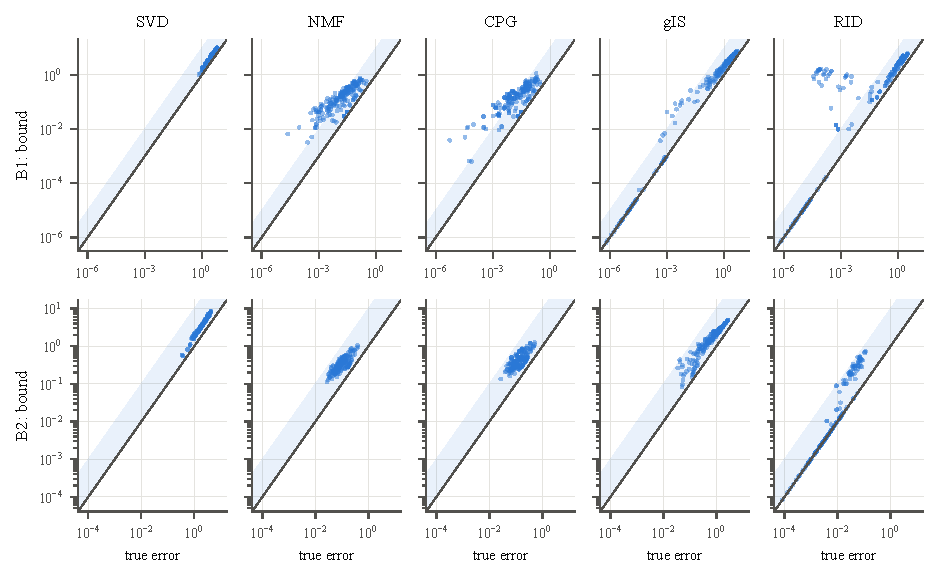
\includegraphics[width=\textwidth]{fig_bound.pdf}
\caption{Bound $\eta_{\mathrm{bound}}$ from Eq.~\eqref{eq:bound1}, evaluated with the exact multiplier norm, against the true energy-norm error for the five dual bases (columns; dual dimensions pooled) on B1 and B2 (rows), with a common range per row. Points on the diagonal would have effectivity one, and the shaded band marks $\theta_{\mathrm{eff}}\in[1,10]$. No point lies below the diagonal, consistent with Theorem~\ref{thm:bound}. The bound is tight for signed SVD and, on B2, for gIS, and loose and weakly ordered for NMF and CPG, which is why the rank correlation of criterion~3 is met reliably only for SVD.}
\label{fig:bound}
\end{figure}

\begin{figure}[htbp]
\centering
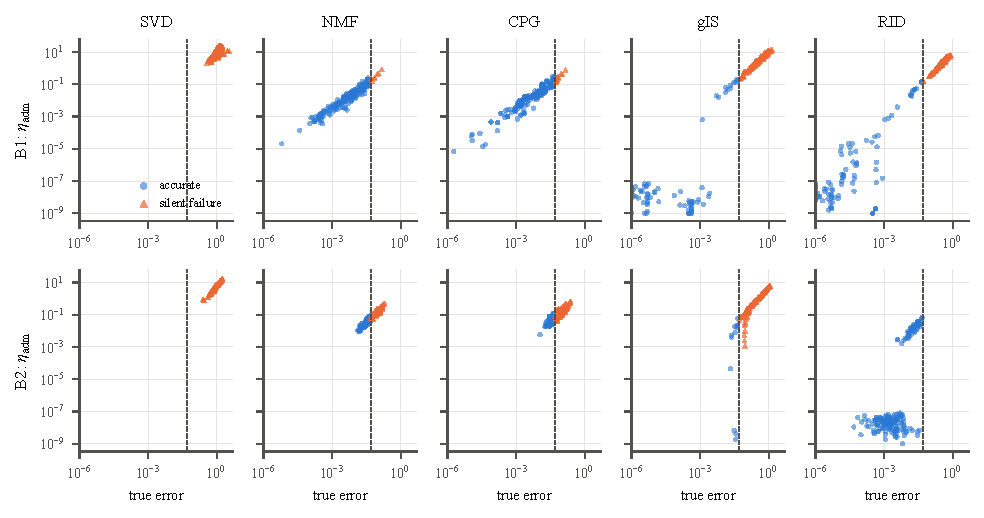
\includegraphics[width=\textwidth]{fig_estimator.pdf}
\caption{Online admissibility indicator $\eta_{\mathrm{adm}}$ (Eq.~\eqref{eq:eta-adm}) against the true energy-norm error for the five dual bases (columns; dual dimensions pooled, seed-42 test queries) on B1 and B2 (rows). Orange triangles are silent failures (reduced KKT residual below $10^{-12}$ and error above $5\%$, dashed line), blue circles are accurate queries. Values of exactly zero are drawn at the axis floor. For signed SVD all queries are silent failures with large indicator values. For NMF and CPG the indicator grows with the error but accurate and failing queries overlap near the dashed line, so a single threshold trades missed failures against false alarms. For gIS and RID the indicator separates the groups well on B1, whereas on B2 a few gIS failures have an indicator far below the bulk of the failures (vertical streak) and cannot be detected by any threshold that also accepts the accurate queries. On B2 the RID queries are all accurate. The indicator is not an error bound: it is a screening statistic whose threshold must be calibrated (Table~\ref{tab:calibration}).}
\label{fig:estimator}
\end{figure}

\begin{figure}[htbp]
\centering
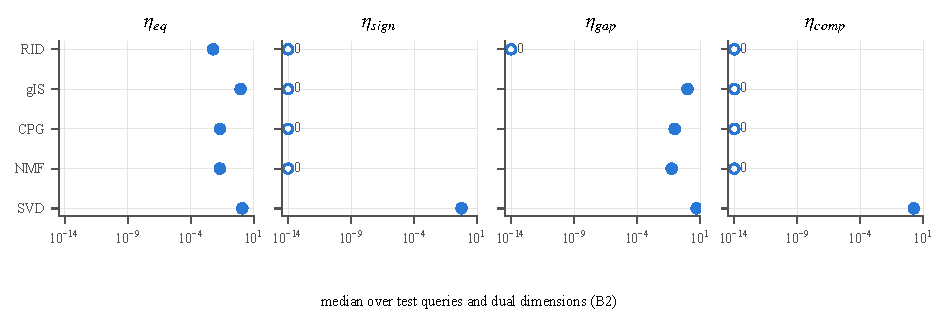
\includegraphics[width=\textwidth]{fig_components.pdf}
\caption{Median value of each estimator component on B2, pooled over test queries and dual dimensions. Hollow markers at the left edge denote values of zero, shown at the axis floor. The non-negative bases (NMF, CPG, gIS, RID) have $\eta_{\mathrm{sign}}=0$ and, in the median, $\eta_{\mathrm{comp}}=0$, whereas signed SVD violates both. The median $\eta_{\mathrm{gap}}$ of RID is zero as well.}
\label{fig:components}
\end{figure}

\begin{figure}[htbp]
\centering
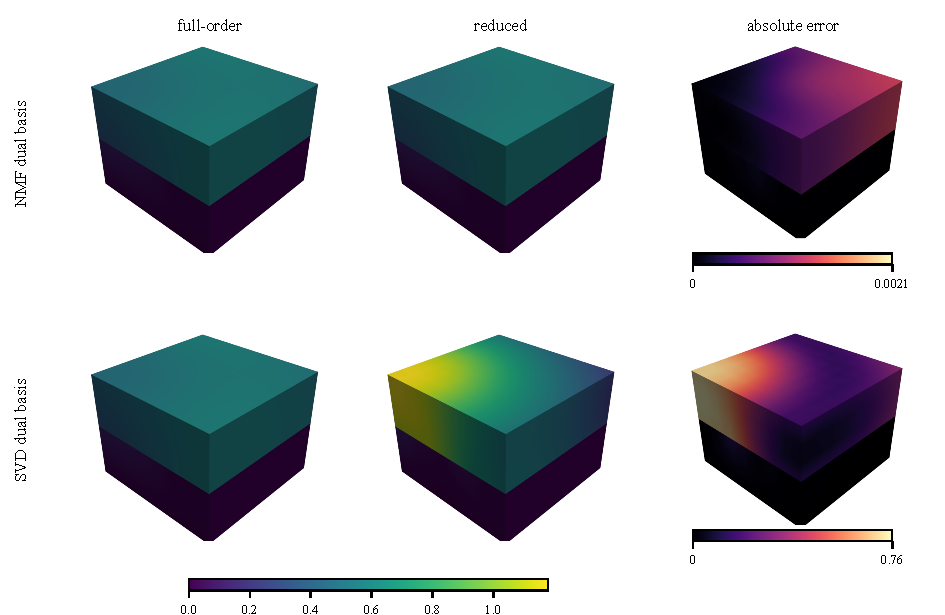
\includegraphics[width=0.86\textwidth]{fig_b3_rom.pdf}
\caption{Full-order, reduced and error displacement magnitude on B3 (illustrative $8\times8$, $3+3$ mesh, drawn on the undeformed mesh because the initial gap is constraint data; the first two columns of both rows share one color range, the error panels have their own). The query was selected from 30 random draws as one on which the SVD model fails (error above $20\%$) while NMF stays accurate, to illustrate the mechanism; it does not represent failure rates (Figures~\ref{fig:silent} and~\ref{fig:bound}). Top: NMF, relative energy error $0.15\%$. Bottom: SVD, error $70\%$ and minimum lifted multiplier $-0.046$.}
\label{fig:b3rom}
\end{figure}
\item
  \textbf{Criterion 2 is met in its scoped form} (queries whose error exceeds the tolerance). Over all queries, effectivity grows like \(\text{err}^{-1/2}\) as errors shrink and is a diagnostic only.
\item
  \textbf{Criterion 4} is met on B2 (both regimes) and on B3 (constant \(K\): 779 vs.\ 1006, ratio 0.77; varying \(K\): 55 vs.\ 86, ratio 0.64; Figure~\ref{fig:breakeven}); it is not evaluable for B1 (fixed size, no sweep). Two caveats apply. The B3 varying-stiffness break-even lies below \(N = 100\), where the reduced dimension (about 20) is comparable to the model size and the sub-millisecond timings are dominated by fixed overheads; the measured speedup is not monotone there (1.24, 1.30, 0.78, 1.16 at \(N = 24\), 40, 63, 105), so the measured break-even is set by a single point. Repeating the B3 sweep moved the measured constant-stiffness break-even from 703 to 1006, so timing uncertainty is of the order of the margin. Moreover the criterion concerns the break-even size only: the predicted speedup is much larger than the measured one at large \(N\) (B3, \(N = 16653\), constant \(K\): 730 predicted vs.\ 55 measured; varying \(K\): 1138 vs.\ 443), so the FLOP model should not be used to quote absolute speedups.

\begin{figure}[htbp]
\centering
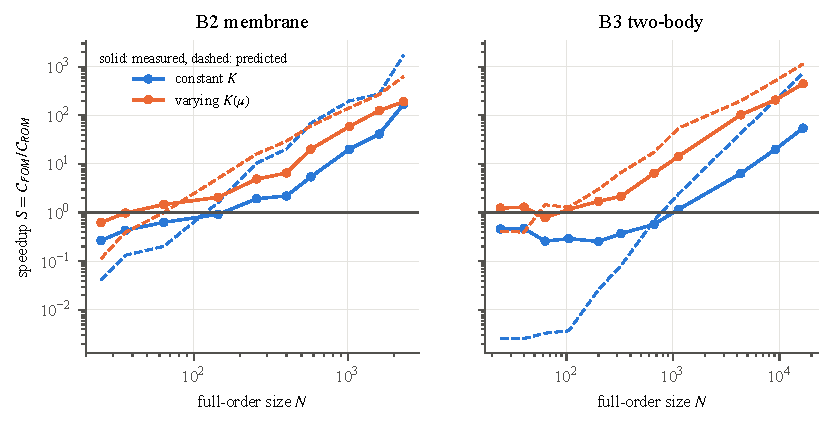
\includegraphics[width=\textwidth]{fig_breakeven.pdf}
\caption{Predicted (dashed, Eqs.~\eqref{eq:cfom}--\eqref{eq:crom}) and measured (solid) speedup against problem size for constant and varying stiffness on B2 and B3. Break-even is the size from which a curve stays above $S=1$; predicted and measured sizes agree within a factor of two in all four cases (ratios $0.78$, $1.72$, $0.77$, $0.64$), the last (below $N=100$) being weakly determined. The model overestimates absolute speedups at large $N$.}
\label{fig:breakeven}
\end{figure}
\item
  \textbf{E5 (B3, default configuration, in-range vs.\ extrapolated load, Figure~\ref{fig:breaker}).} With \(\tau_{\text{adm}}\) calibrated on validation queries, the admissibility screening accepted no unsafe answer for NMF and CPG at \(r_\lambda \in \{8,16\}\) (0 misses). On in-range queries about 4\% fall back to the full-order solve and the speedup is about 16--18\(\times\). On extrapolated loads 96--100\% fall back and the speedup is about 1\(\times\): the breaker keeps answers safe but removes the acceleration. Only 4\% of in-range queries were unsafe without the breaker, so the in-range zero-miss result rests on very few positives.

\end{itemize}

\begin{figure}[htbp]
\centering
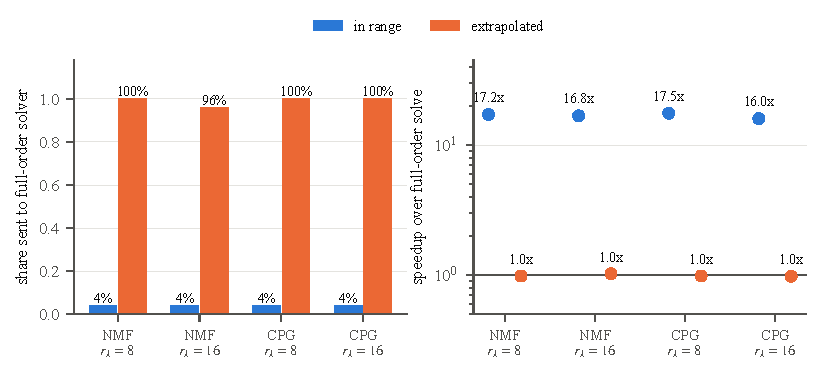
\includegraphics[width=\textwidth]{fig_breaker.pdf}
\caption{Circuit breaker on B3 (NMF and CPG, $r_\lambda\in\{8,16\}$, $\tau_{\mathrm{adm}}$ calibrated on validation queries; 25 queries per set). Left: share sent to the full-order solver. Right: speedup including the fallback cost. In-range queries are almost all accepted (about $16$--$18\times$); extrapolated ones are almost all rejected, which keeps answers safe but removes the acceleration. Few in-range queries ($4\%$) were unsafe, so zero misses there rests on few positives.}
\label{fig:breaker}
\end{figure}

\FloatBarrier
% ======================================================================
\section{Conclusion and Practical Guidelines}
\label{sec:conclusion}

\hypertarget{summary-of-contributions}{%
\subsection{Summary of Contributions}\label{summary-of-contributions}}

Projection-based reduced-order models for unilateral contact problems may exhibit a significant discrepancy between convergence of the reduced system and the physical admissibility of the reconstructed solution. In particular, the reduced solver may satisfy its projected KKT conditions to machine precision (residuals below \(3 \times 10^{-14}\) in our experiments) while the lifted displacement--multiplier pair \((\tilde{u}, \tilde{\lambda}) = (V u_r, U \lambda_r)\) violates the full-order contact constraints, with relative energy-norm errors of order one \cite{balajewicz2016projection, benaceur2020reduced}.

This work makes three contributions.

\begin{enumerate}
\def\labelenumi{\arabic{enumi}.}
\tightlist
\item
  \textbf{Lifted Error Bound and Admissibility Screening:} Adapting constant-sign multiplier residual decompositions \cite{hild2007residual, dabaghi2020posteriori, banz2024generic, fontana2024guaranteed, banz2026posteriori} to lifted reduced-order pairs under general rectangular constraint matrices \(B(\mu) \in \mathbb{R}^{n_c \times N}\) (removing the bijective operator restriction of \cite{zhang2014duality}), we proved an energy-norm \emph{a posteriori} upper bound composed of a dual-norm equilibrium residual (\(\eta_{\text{eq}}\)) and three contact-interface terms measuring multiplier sign violation (\(\eta_{\text{sign}}\)), primal interpenetration (\(\eta_{\text{gap}}\)), and complementarity defect (\(\eta_{\text{comp}}\)). The resulting online admissibility indicator \(\eta_{\text{adm}} = \eta_{\text{sign}} + \eta_{\text{gap}} + \sqrt{\eta_{\text{comp}}}\) can be evaluated in \(\mathcal{O}(n_c (r_u + r_\lambda))\) operations without full-order bulk quantities and serves as an online admissibility screening indicator. In the experiments of Section~\ref{sec:experiments} the bound (with the exact multiplier norm) held on every test query, but over five seeds the calibrated threshold missed some silent failures for most bases in several seeds, and the bound ranked errors reliably only for SVD; zero false negatives is therefore not claimed.
\item
  \textbf{Controlled Cross-Basis Benchmark:} Evaluating signed SVD with primal rank repair \cite{leberre2022condition}, non-negative matrix factorization (NMF) \cite{balajewicz2016projection}, cone-projected greedy (CPG) \cite{benaceur2020reduced}, greedy index selection (gIS) \cite{sambataro2026model, kollepara2024sparse}, and reduced integration domain (RID) restriction \cite{fauque2018hybrid, leberre2022condition} on identical snapshot sets compares offline construction cost, dual non-negativity, primal rank-repair overhead and accuracy (Table~\ref{tab:e3}); out-of-range robustness was tested for all five bases on B1 and B2 and for NMF and CPG on the three-dimensional problem (experiment E5).
\item
  \textbf{FLOP- and Iteration-Aware Break-Even Cost Model:} By accounting for dense reduced Schur-complement factorization, unit-vector rank-repair enrichment \(r_{\text{rep}}\) \cite{leberre2022condition}, and active-set iteration growth \(k_{\text{ROM}}\) relative to sparse full-order solvers \cite{franceschini2022block, pawar2025efficient}, our cost model predicts the problem dimensions and active contact-zone fractions at which Lagrange-multiplier contact ROMs yield wall-clock speedups. Predicted and measured break-even sizes agree within a factor of two on the membrane (ratios 0.78 and 1.72) and on B3 (0.77 for constant and 0.64 for varying stiffness). The latter crossover lies below \(N = 100\) and is weakly determined. B1 was not scored against the model; only its measured speedup was swept, in the mesh-size study. Predicted speedups exceed measured ones at large sizes by up to an order of magnitude. A ten-repeat re-run (Table~\ref{tab:timing}) reproduces the break-even sizes within bootstrap intervals in most cases. However, the varying-stiffness ratio on the membrane rises to 1.97, and the single-run B3 value lies outside the interval of the re-run, so the factor-of-two agreement should be read as approximate.
\end{enumerate}

The evidence supports the framework as a diagnostic and planning tool inside the tested range: the error bound holds with the exact multiplier norm on every audited query, signed dual bases fail silently, non-negative bases reduce but do not remove the hazard, and the break-even sizes of the cost model are located within roughly a factor of two for direct full-order solvers. It does not support a general claim of certified online reliability. The online-usable bound depends on an offline multiplier-norm constant, the interface-based screening indicator detects most but not all silent failures at the price of false alarms that are high on some benchmarks, its threshold needs validation queries that contain failures, and the cost model predicts break-even sizes, not speedups. Results on other geometries, contact laws, solvers and hardware may differ.

\subsection{Discussion}\label{sec:discussion}

The observations are in Section~\ref{sec:experiments}. Here we interpret them. The explanations are plausible readings of the data and were not isolated by dedicated experiments.

\paragraph{Performance of the dual-basis strategies.} The signed SVD basis does not preserve multiplier non-negativity, which allows negative components in the lifted multiplier vector and a large sign indicator $\eta_{\mathrm{sign}}$; the bound increases accordingly. NMF and CPG remove the sign defect by construction, which is consistent with the comparatively smaller errors observed in the experiments. Their columns do not enforce complementarity at individual contact points, and on the membrane the error exhibits a plateau of approximately $2$--$3\%$ as the dimension grows. gIS keeps unit vectors at selected contact indices, so its errors are large until the selected contact indices adequately represent the active contact region; on B1 the median error falls from $0.05$ at $r_\lambda = 16$ to $3\times10^{-6}$ at $24$, a sharp transition rather than a gradual one. RID retains all contact rows of the selected elements, which gives the highest accuracy at high dimension ($10^{-3}$ or below) but at the price of an effective dual dimension of 23 (B1) and 98 (B2) at nominal 16 and of up to 78 repair vectors.

\paragraph{Computational break-even behaviour.} Our measured break-even sizes are about $N = 150$ (membrane, constant stiffness), $30$--$40$ (membrane, varying stiffness), about $700$--$1000$ (two-body, constant stiffness) and $67$--$86$ (two-body, varying stiffness), for direct full-order solvers and the code and machine used. With constant stiffness, a computational advantage is observed only beyond a sufficiently large problem size, because the full-order cost then consists of the active-set solve alone. The savings are reduced by the fallback: on the membrane at $N = 324$ the hybrid rule sends between $7\%$ and $94\%$ of the queries to the full-order solver depending on the basis, and the net speedup of the screened ROM is below one for constant stiffness. The offline cost of the dual basis is small in absolute terms at these sizes (1--2\,ms for SVD, about 140--190\,ms for NMF), and primal repair is the dominant effect on the online cost only for RID on the membrane.

\paragraph{Limitations and applicability.} The interface-based screening indicator can miss inadmissible solutions, and some bases give high false-alarm rates; the computational advantage depends on the benchmark and the problem size; the time-dependent extension was not demonstrated; and changing contact geometries and contact-patch translation were not studied. These are developed in Section~\ref{limitations-and-future-work}.

\hypertarget{practical-guidelines-for-contact-rom-deployment}{%
\subsection{Practical Guidelines for Contact ROM Deployment}\label{practical-guidelines-for-contact-rom-deployment}}

Based on the theoretical bounds in Section 3 and the cost scaling in Section 4, we summarize five guidelines for practitioners deploying Lagrange-multiplier reduced contact models:

\begin{enumerate}
\def\labelenumi{\arabic{enumi}.}
\tightlist
\item
  \textbf{Never rely solely on reduced KKT residuals for online acceptance:}
  Evaluate the online admissibility indicator \(\eta_{\text{adm}}\) after lifting \((u_r, \lambda_r)\) as an additional screening measure. Because the indicator is empirical and may miss inadmissible predictions, it should not be treated as a standalone guarantee of reliability. When it exceeds the calibrated screening threshold, reject the reduced prediction and invoke the full-order fallback \cite{dabaghi2020posteriori}. If such rejections occur frequently, the reduced basis may require additional enrichment \cite{leberre2022condition} or reconstruction.
\item
  \textbf{Enforce dual non-negativity by construction (\(\eta_{\text{sign}} = 0\)) whenever possible:}
  Avoid truncated signed SVD dual bases unless paired with strict online \(\eta_{\text{sign}}\) monitoring and aggressive interface enrichment. When offline NMF cost is acceptable, NMF \cite{balajewicz2016projection} provides compact non-negative dual bases; when fast offline assembly or exact pointwise complementarity at key contact nodes is prioritized, greedy index selection (gIS) \cite{sambataro2026model, kollepara2024sparse} and cone-projected greedy (CPG) \cite{benaceur2020reduced} eliminate sign violations with low offline overhead. Non-negativity is not sufficient, however: NMF errors still exceeded \(5\%\) on \(40\%\) of the B2 test queries (Figure~\ref{fig:silent}), so the online indicator remains necessary.
\item
  \textbf{Audit primal rank-repair enrichment against active contact size before deployment:}
  In constant-stiffness problems where \(B K^{-1} B^T\) can be precomputed offline \cite{pawar2025efficient}, dense reduced algebra scales cubically with the enriched primal dimension \(r_u = r_{u,0} + r_{\text{rep}}\) \cite{leberre2022condition}. Verify via the break-even inequality in Section 4.2 that \(r_u\) remains substantially smaller than the active contact count \(m_{\text{act}}\); otherwise, a reduced-space active-set solver on the precomputed full-order compliance matrix \cite{franceschini2022block} will outperform the projection ROM.
\item
  \textbf{Calibrate the screening threshold on queries that contain failures and treat it as valid only within the calibrated range:}
  The threshold is an empirical quantity. It cannot be calibrated when the validation set contains no silent failure, its recall depends on the number of validation queries, and in our out-of-range tests it missed most silent failures of one basis whose validation set had none. Report the recall and false-alarm rate together with the number of validation queries, and re-calibrate when the parameter range changes.
\item
  \textbf{Use \(\eta_{\text{eq}}\) offline to enrich bulk primal modes during greedy training:}
  Because \(\eta_{\text{adm}}\) monitors interface admissibility alone, use the full four-component bound \(\eta_{\text{bound}}\) (including \(\eta_{\text{eq}}\)) during offline greedy sampling \cite{benaceur2020reduced, zhang2014duality} so that interior bulk deformation modes are enriched alongside contact interface modes.
\end{enumerate}

\hypertarget{limitations-and-future-work}{%
\subsection{Limitations and Future Work}\label{limitations-and-future-work}}

The conclusions should be interpreted within the numerical scope of the study. The main tables use a single random seed (42) with 40 test and 40 validation queries per benchmark, and the five-seed check of Table~\ref{tab:robust} shows that the outcome of the detection criterion depends on the seed. The calibration study of Section~\ref{results-and-acceptance-outcome} (eight seeds, bootstrap intervals over seeds) quantifies this uncertainty on B1 and B2 only, and B3 was not repeated over seeds. Threshold calibration requires validation queries that contain silent failures, and several non-negative basis entries had none. The threshold was calibrated in range, and outside the training range its performance deteriorated for some bases (Table~\ref{tab:extrap}). An in-sample validation set was not evaluated.

The benchmarks and the cost model have further limitations. Three-dimensional results come from one mesh family of a single two-body geometry, and no second, independent three-dimensional configuration was run. Out-of-range queries were tested for one range of loads, obstacle shapes and indenter positions on B1 and B2, and for NMF and CPG only on B3. The dual-basis comparison at matched cost rests on one seed per benchmark, and the mesh-size study used a fixed dual dimension. The break-even model is validated on the membrane and on the three-dimensional problem; on B1 only the measured speedup was swept. The B3 varying-stiffness crossover is weakly determined at small sizes, the ten-repeat timing study shows run-to-run differences of up to about 40\% in the measured break-even and a varying-stiffness ratio on the membrane of 1.97, and the model overestimates absolute speedups at large sizes by up to an order of magnitude and assumes direct full-order solvers (Section~\ref{cost-model-assumptions}).

The effectivity and correlation results use the bound with the exact multiplier norm of the full-order solution, which is a validation quantity. The online-usable version with the offline constant \(C_\lambda\) is rigorous only while the query multiplier norm stays below \(C_\lambda\). It fell below the true error on up to \(0.5\%\) of in-range test queries for gIS and RID on B1 and on up to \(1.5\%\) (B1) and \(3.5\%\) (B2) of the out-of-range queries.

Two directions warrant further investigation. First, the experiments focus on frictionless unilateral contact; extending the constant-sign multiplier decomposition to Coulomb frictional contact \cite{niakh2024reduced} requires coupling normal traction admissibility with tangential friction-cone projection residuals. Second, integrating the online admissibility screening \(\eta_{\text{adm}}\) into an automated, on-the-fly basis enrichment loop for large-scale 3D nonlinear elastoplastic and substructured dynamic contact \cite{koller2021hyper, aresdeparga2023petrov, manvelyan2026inference} is a possible next step; it would need the bound with a valid multiplier-norm estimate and a calibrated screening threshold before any claim of certification could be made. The time-dependent extension was considered but not performed and is also left to future work.


{\small
\bibliographystyle{elsarticle-num}
\bibliography{references} }

\end{document}
